\onecolumn
\section{Acknowledgements to open-source software projects}

We would like to give credit to some essential software projects we used extensively for our work. We would like to at least name Pyro \citep{bingham2019pyro}, NumPyro \citep{phan2019numpyro}, Numpy \citep{harris2020numpy}, PyTorch \citep{pytorch2019} and Scikit Learn \citep{scikit} as essential tool boxes for the experiments we have conducted and the analyses we have performed.

\section{Experimental set-up}\label{app:hyperparameters}
\subsection{Objectives}

An overview of the objectives used in the experiments as described in Section \ref{sec:experiments} is given in Table \ref{tab:objectives}. The hyperparameter settings of the separate runs are summarised in Table \ref{tab:objectives-hp}. The total number of experiments ran on the Penn Treebank dataset is 23 and on binarised MNIST 66.

% Objective equations
\begin{table*}[!htb]
    \centering
    \scriptsize
    \begin{tabular}{ccc}
        \toprule
        Objective (hyperparameters) & Equation \\
        \midrule
        $\beta$-VAE \cite{higgins2016beta} ($\beta$) & $\max_{\theta, \phi} \mathcal{L}_{\beta\text{-VAE}}(\theta, \phi) = \mathbb{E}_{q_{Z|X=x}}[\log p_{X|Z=z}(\phi)] - \beta \KL(q_{Z|X=x}(\theta)||p_{Z}(\phi))$ \\
        \addlinespace[0.5em]
        Info-VAE \cite{zhao2017infovae} ($\lambda_\text{rate}$, $\lambda_\text{MMD}$) & $\max_{\theta, \phi} \mathcal{L}_{\text{Info-VAE}}(\theta, \phi) = \mathbb{E}_{q_{Z|X=x}}[\log p_{X|Z=z}(\phi)] - \lambda_\text{rate} \KL(q_{Z|X=x}(\theta)||p_{Z}(\phi)) + \lambda_\text{MMD} \text{MMD}$\\
        \addlinespace[0.5em]
        Free-bits-VAE \cite{kingma2016improved}  ($\lambda_\text{FB}$) & $\max_{\theta, \phi} \mathcal{L}_{\text{FB-VAE}}(\theta, \phi) = \mathbb{E}_{q_{Z|X=x}}[\log p_{X|Z=z}(\phi)] - \max( \KL(q_{Z|X=x}(\theta)||p_{Z}(\phi)), \lambda_{\text{FB}})$ \\
        \bottomrule
    \end{tabular}
    \caption{Overview of the objectives with their hyperparameters used for the experiments.}
    \label{tab:objectives}
\end{table*}

% hyperparameters
\begin{table*}[!htb]
    \centering
    \begin{tabular}{c||c|c}
        \toprule
         & PTB & MNIST \\
         \midrule
        $\beta \in$ & $\{0.0, 0.25, 0.5, 0.75, 1.0, 2.0\}$ & $\{0.0, 0.25, 0.5, 0.75, 1.0, 1.5, 2.0, 5.0, 10.0\}$ \\
        \addlinespace[0.5em]
        $(\lambda_{\text{rate}}, \lambda_{\text{MMD}}) \in$ & $\{1, 10, 100\} \times \{0.1, 0.5, 1.0, 2.0\} $ & $\{1, 10, 100\} \times \{0.1, 0.5, 1.0, 2.0, 5.0, 10.0\}$ \\
        \addlinespace[0.5em]
        $\lambda_{\text{FB}} \in$ & $\{4, 8, 16, 32, 64\}$ & $\{4, 8, 16, 24, 32, 40\}$ \\
        \bottomrule
    \end{tabular}
    \caption{The hyperparameters for the objectives outlined in Section \ref{sec:experiments}}.
    \label{tab:objectives-hp}
\end{table*}

\section{Architectures}\label{app:architectures}

\subsection{Binarised MNIST}
\subsubsection{Gated CNN Encoder}

We use the the gated convolutional encoder from \citet{van2018sylvester} with two additional linear layers to map to the location and scale parameters of the approximate posterior. The gating mechanism can be expressed as follows, where $\ast$ denotes convolution and $\odot$ denotes element-wise multiplication:

% GatedConv2D equation
\begin{equation*}
    \mathbf{y}_{\text{GatedConv2D}} = (\mathbf{V} \ast \mathbf{x} + \mathbf{b}) \odot \sigma(\mathbf{W} \ast \mathbf{x} + \mathbf{c})
\end{equation*}

The encoder consists of the following GatedConv2d layers, with the parameters between parentheses denoting number of input channels, number of output channels, kernel size, stride and padding respectively:

% Gated CNN Encoder layer summary
\begin{itemize}
    \item GatedConv2d(1,  32,  5, 1, 2)
    \item GatedConv2d(32, 32,  5, 2, 2))
    \item GatedConv2d(32, 64,  5, 1, 2)
    \item GatedConv2d(64, 64,  5, 2, 2)
    \item GatedConv2d(64, 64,  5, 1, 2)
    \item GatedConv2d(64, 256, 7, 1, 0)
\end{itemize}

\subsubsection{Gated CNN.T decoder}

Similarly, for the simple decoder architecture we follow \citet{van2018sylvester} by using GatedConvTranspose2d units as the main building block to map the sampled latent representation $\mathbf{z}$ to the parameters of Bernoulli distributions to model the binary pixel values. The full architecture can be summarised as follows, where the parameters of the GatedConvTranspose2d, in order, denote the number of input channels, the number of output channels, kernel size, stride, padding and (optionally) the output padding:

% Gated CNN.T Decoder layer summary
\begin{itemize}
    \item GatedConvTranspose2d(10, 64, 7, 1, 0)
    \item GatedConvTranspose2d(64, 64, 5, 1, 2)
    \item GatedConvTranspose2d(64, 32, 5, 2, 2, 1)
    \item GatedConvTranspose2d(32, 32, 5, 1, 2)
    \item GatedConvTranspose2d(32, 32, 5, 2, 2, 1)
    \item GatedConvTranspose2d(32, 32, 5, 1, 2)
    \item GatedConvTranspose2d(32, 1, 1, 1, 0)
\end{itemize}

\subsubsection{PixelCNN++ decoder}

We follow \cite{alemi2018fixing} in slightly modifying the work of \cite{salimans2017pixelcnn++} to function as a VAE decoder architecture. The latent $\mathbf{z}$ is added to the decoder via a conditioning mechanism in all the GatedResNet blocks. This mechanism projects the latent to the spatial dimensions of the feature maps that are the output of this block ($\mathbf{x_1}$ and $\mathbf{x_2}$) and and adds the projections to all channels identically before the gating mechanism. The operation can be described as:

\begin{equation*}
    \mathbf{y_{\text{GatedResNet}}} = (\mathbf{x_1} + \mathbf{V}^T \mathbf{z}) \odot \sigma(\mathbf{x_2} + \mathbf{W}^T \mathbf{z})
\end{equation*}

We use three down-sampling blocks ($28 \rightarrow 14 \rightarrow 7$) and three up-sampling blocks ($7 \rightarrow 14 \rightarrow 28$) with skip connections between blocks of equal spatial dimensionality. Each block consists of 2 GatedResNet units and the number of filters is set to 64. We adapt the output layer to output the parameters of the Bernoulli distribution over the spatial dimensions of the image (28 x 28).

\subsection{Penn Treebank}
\subsubsection{Distil RoBERTa Encoder} 

For the encoder we use a transformer architecture, specifically a RoBERTa Encoder architecture \cite{liu2019roberta}\footnote{We use the implementation of Huggingface described here: \url{https://huggingface.co/docs/transformers/model_doc/roberta}} and initialise with weights that are obtained by means of knowledge distillation \cite{Sanh2019DistilBERTAD}.\footnote{Specifically we use the weights from the \texttt{distil-roberta} checkpoint: \url{https://huggingface.co/distilroberta-base}} We add a pooling layer that maps the output of the encoder to the parameters of the approximate posterior distribution.

\subsubsection{Adapted Distil Roberta Decoder} 
For the decoder we use the same basis as for the encoder. We adapt its architecture following the work of \cite{li2020optimus} to incorporate the latent representations via two mechanisms: the attention mechanism and the embedding mechanism. For the former, the latent representation is mapped to the dimensionality of the hidden layers for every layer in the model and added via the attention mechanism in the form of key and value vectors. For the latter mechanism, the latent representation is simply projected to the dimensionality of the hidden layers and is summed with the initial hidden states of the model, right after embedding the tokens. This operation is the same for all positions in the sequence. At the output, a language model head is added to map the output of the RoBERTa block to the parameters of a Categorical distribution that models the token distributions per sequence position. Auto-regressive masking is used to prevent the model to have access to information beyond the current token position.


\section{Latent structure models and lppd statistics}\label{app:latent-structure-models}
\subsection{Graphical models}

Table \ref{tab:BDA_diagrams} shows the graphical models of the latent structure models used for our analysis.

% \begin{table*}[t]
    \centering
    \small
    \begin{tabular}{ ccccc } 
    \toprule
    MNIST & \multicolumn{2}{c}{PTB} & Latent  \\
    
    \cmidrule(lr){1-1}
    \cmidrule(lr){2-3}
    \cmidrule(lr){4-4} \\
    
    % MNIST
    \begin{tikzpicture}[x=1.3cm, y=0.8cm]
        % NODES
        % -----------------
      
        \node[obs]                   (x_n)    {$x_n$} ; %
        \node[latent, above=of x_n, yshift=+0.5cm]  (p_kd)   {$p_{k, d}$} ; %
        \node[latent, left=of x_n]   (c_n)    {$c_n$} ;
        
        \node[const, above=of p_kd, xshift=-0.5cm]  (beta_p) {$\alpha_p$}; 
        \node[const, above=of p_kd, xshift=+0.5cm]  (alpha_p) {$\beta_p$};
        
        % PLATES
        % -----------------
        
        % Component plate
        {\tikzset{plate caption/.append style={below=0.15cm of #1.south east}}
        \plate[minimum width=1.45cm, minimum height=1.55cm, yshift=+0.1cm, xshift=-0.05cm]{component_plate}{(p_kd)}{\footnotesize $K$};}
        
        % Pixel plate
        % to circumvent overlapping labels
        {\tikzset{plate caption/.append style={below=0.65cm of #1.south east, xshift=+0.05cm}}
        \plate[minimum width=1.85cm, xshift=-0.1cm, minimum height=4.25cm, yshift=+0.1cm]{pixel_plate}{(p_kd)(x_n)}{\footnotesize $D$};}
        
        % Data point plate
        {\tikzset{plate caption/.append style={below=0.1cm of #1.south east, xshift=+0.1cm}}
        \plate[minimum height=1.6cm, yshift=+0.15cm]{data_plate}{(c_n)(x_n)}
        {\footnotesize $N$};}
        
        % EDGES
        % -----------------
        
        \edge{p_kd}{x_n}
        \edge{alpha_p, beta_p}{p_kd}
        \edge{c_n}{x_n}
      
    \end{tikzpicture}

    
    & 
    % PTB diagram 1 - Sequence length model 
    \begin{tikzpicture}[x=1.2cm, y=0.8cm]
      \node[obs]                   (x_n)            {$x_n$};
      \node[latent, above=of x_n]  (c_n)            {$c_n$};
      \node[latent, above=of c_n]  (theta)          {$\vec{\theta}$};
      \node[const, above=of theta] (alpha_theta)    {$\alpha_\theta$};
    
      \node[latent, left=of c_n, xshift=0.35cm] (rate_k)  {$r_k$}; %
      \node[const, above=of rate_k, xshift=-0.5cm]  (a_rate) {$a_\phi$}; 
      \node[const, above=of rate_k, xshift=+0.5cm]  (b_rate) {$b_\phi$}; %
    
      \plate[minimum height=2.8cm, minimum width=1.35cm]{plate_obs} {(c_n) (x_n) } {$N$};
      \plate[minimum height=1.55cm, yshift=+0.1cm, minimum width=1.35cm]{plate_rate} {(rate_k)} {$K$}
      
      \edge {c_n,rate_k} {x_n} ; %
      \edge {theta} {c_n}
      \edge {alpha_theta} {theta}
      \edge {a_rate}{rate_k}
      \edge {b_rate}{rate_k}
    \end{tikzpicture} 
    
    & 
    % PTB diagram 2 - LDA model \\ 
    \begin{tikzpicture}[x=1.3cm, y=0.8cm]
        % NODES
        % -----------------
        
        \node[const] (beta) {$\beta_\phi$};
        \node[latent, above=of beta, yshift=+0.25cm] (phi_k) {$\vec{\phi}_k$};
        \node[obs, above=of phi_k, yshift=0.8cm] (x_mn) {$x_{mn}$};
        \node[latent, above=of x_mn] (c_mn) {$c_{mn}$};
        \node[latent, above=of c_mn] (theta_m) {$\vec{\theta}_m$};
        \node[const, above=of theta_m] (alpha) {$\alpha_\theta$};
        
        % PLATES
        % -----------------
        
        % Document plate
        {\tikzset{plate caption/.append style={below=0.85cm of #1.south east}}
        \plate[minimum width=2.1cm, minimum height=5.4cm, yshift=+0.1cm, xshift=0.0cm]{document_plate}{(theta_m)(c_mn)(x_mn)}{$M$}}
        
        % Token plate
        {\tikzset{plate caption/.append style={below=0.3cm of #1.south east}}
        \plate[minimum width=1.6cm, xshift=+0.0cm, yshift=0.1cm, minimum height=3.4cm]{token_plate}{(c_mn)(x_mn)}{$N$}}
        
        % Topic plate
        {\tikzset{plate caption/.append style={below=0.4cm of #1.south east}}
        \plate[minimum width=2.1cm, minimum height=1.6cm, yshift=-0.05cm]{topic_plate}{(phi_k)}{$K$}}
        
        % EDGES
        % -----------------
        \edge{alpha}{theta_m}
        \edge{theta_m}{c_mn}
        \edge{c_mn}{x_mn}
        \edge{phi_k}{x_mn}
        \edge{beta}{phi_k}
  
    \end{tikzpicture}
    
    &
    % Latent analysis
    \begin{tikzpicture}[x=1.3cm, y=0.8cm]
        % NODES
        % -----------------
        
        
        
        
        \node[latent] (d) {$\vec{d}$};
        
        \node[latent, above=of d, yshift=+0.25cm] (lambda_k) {$\vec{\lambda}_k$} ;
        
        \node[latent, below=of lambda_k, yshift=-0.25cm, xshift=+1.0cm] (mu) {$\vec{\mu}$} ;
        \node[latent, below=of lambda_k, yshift=-0.25cm, xshift=-1.0cm] (f) {$\vec{f}$} ;
        
        \node[obs, above=of lambda_k, yshift=0.8cm] (z_mn) {$\vec{z}_{mn}$} ;
        \node[latent, above=of z_mn] (c_mn) {$c_{mn}$} ;
        \node[latent, above=of c_mn] (theta_m)  {$\vec{\theta}_m$} ;
        \node[const, above=of theta_m] (alpha)    {$\alpha_\theta$} ;
        
        \node[const, below= of mu] (mu_prior) {$\{ \alpha_\mu \}$};
        \node[const, below= of f] (f_prior) {$\{ \alpha_f \}$};
        \node[const, below= of d] (d_prior) {$\{ \alpha_d \}$};
        
        % PLATES
        % -----------------
        
        % Document plate 
        % above right = 2cm and 3cm of a
        {\tikzset{plate caption/.append style={below = 0.85cm of #1.south east}}
        \plate[minimum width=2.1cm, minimum height=5.4cm, yshift=+0.1cm, xshift=0.0cm]{document_plate}{(theta_m)(c_mn)(z_mn)}{$M$}}
        
        % Latent representation plate
        {\tikzset{plate caption/.append style={below = 0.45cm of #1.south east}}
        \plate[minimum width=1.6cm, xshift=+0.0cm, yshift=0.1cm, minimum height=3.4cm]{token_plate}{(c_mn)(z_mn)}{$N$}}
        
        % Component plate
        {\tikzset{plate caption/.append style={above right = -0.15cm and 0.15cm of #1.north east}}
        \plate[minimum width=2.0cm, minimum height=1.5cm, yshift=-0.25cm, xshift=-0.15cm]{topic_plate}{(lambda_k)}{$K$}}
        
        % EDGES
        % -----------------
        \edge{alpha}{theta_m}
        \edge{theta_m}{c_mn}
        \edge{c_mn}{z_mn}
        \edge{lambda_k}{z_mn}
        \edge{mu}{lambda_k}
        \edge{d}{lambda_k}
        \edge{f}{lambda_k}
        
        \edge{mu_prior}{mu}
        \edge{d_prior}{d}
        \edge{f_prior}{f}
  
    \end{tikzpicture}
    \\
    \\
    Digit identity & Sequence length & Topic structure & Prior structure \\
    \bottomrule
    \end{tabular}
    \caption{This table shows the latent structure models described in Section \ref{subsec:bda_models} used to demonstrate the proposed evaluation methodology. The captions denote the latent structure that is captured by each individual model and is represented graphically by the latent variable $c$.}
    \label{tab:BDA_diagrams}
 \end{table*}
\begin{table*}[!htb]
    \centering
    \small
    \begin{tabular}{ ccccc } 
    \toprule
    MNIST & \multicolumn{2}{c}{PTB} & Latent  \\
    
    \cmidrule(lr){1-1}
    \cmidrule(lr){2-3}
    \cmidrule(lr){4-4} \\
    
    % MNIST
    \begin{tikzpicture}[x=1.3cm, y=0.8cm]
        % NODES
        % -----------------
      
        \node[obs]                   (x_n)    {$x_n$} ; %
        \node[latent, above=of x_n, yshift=+0.5cm]  (p_kd)   {$p_{k d}$} ; %
        \node[latent, left=of x_n]   (c_n)    {$c_n$} ;
        
        \node[const, above=of p_kd, xshift=-0.5cm]  (beta_p) {$\alpha_p$}; 
        \node[const, above=of p_kd, xshift=+0.5cm]  (alpha_p) {$\beta_p$};
        
        % PLATES
        % -----------------
        
        % Component plate
        {\tikzset{plate caption/.append style={below=0.15cm of #1.south east}}
        \plate[minimum width=1.45cm, minimum height=1.55cm, yshift=+0.1cm, xshift=-0.05cm]{component_plate}{(p_kd)}{\footnotesize $K$};}
        
        % Pixel plate
        % to circumvent overlapping labels
        {\tikzset{plate caption/.append style={below=0.65cm of #1.south east, xshift=+0.05cm}}
        \plate[minimum width=1.85cm, xshift=-0.1cm, minimum height=4.25cm, yshift=+0.1cm]{pixel_plate}{(p_kd)(x_n)}{\footnotesize $D$};}
        
        % Data point plate
        {\tikzset{plate caption/.append style={below=0.1cm of #1.south east, xshift=+0.1cm}}
        \plate[minimum height=1.6cm, yshift=+0.15cm]{data_plate}{(c_n)(x_n)}
        {\footnotesize $N$};}
        
        % EDGES
        % -----------------
        
        \edge{p_kd}{x_n}
        \edge{alpha_p, beta_p}{p_kd}
        \edge{c_n}{x_n}
      
    \end{tikzpicture}

    
    & 
    % PTB diagram 1 - Sequence length model 
    \begin{tikzpicture}[x=1.2cm, y=0.8cm]
      \node[obs]                   (x_n)            {$x_n$};
      \node[latent, above=of x_n]  (c_n)            {$c_n$};
      \node[latent, above=of c_n]  (theta)          {$\vec{\theta}$};
      \node[const, above=of theta] (alpha_theta)    {$\alpha_\theta$};
    
      \node[latent, left=of c_n, xshift=0.35cm] (rate_k)  {$r_k$}; %
      \node[const, above=of rate_k, xshift=-0.5cm]  (a_rate) {$a_\phi$}; 
      \node[const, above=of rate_k, xshift=+0.5cm]  (b_rate) {$b_\phi$}; %
    
      \plate[minimum height=2.8cm, minimum width=1.35cm]{plate_obs} {(c_n) (x_n) } {$N$};
      \plate[minimum height=1.55cm, yshift=+0.1cm, minimum width=1.35cm]{plate_rate} {(rate_k)} {$K$}
      
      \edge {c_n,rate_k} {x_n} ; %
      \edge {theta} {c_n}
      \edge {alpha_theta} {theta}
      \edge {a_rate}{rate_k}
      \edge {b_rate}{rate_k}
    \end{tikzpicture} 
    
    & 
    % PTB diagram 2 - LDA model \\ 
    \begin{tikzpicture}[x=1.3cm, y=0.8cm]
        % NODES
        % -----------------
        
        \node[const] (beta) {$\beta_\phi$};
        \node[latent, above=of beta, yshift=+0.25cm] (phi_k) {$\vec{\phi}_k$};
        \node[obs, above=of phi_k, yshift=0.8cm] (x_mn) {$x_{mn}$};
        \node[latent, above=of x_mn] (c_mn) {$c_{mn}$};
        \node[latent, above=of c_mn] (theta_m) {$\vec{\theta}_m$};
        \node[const, above=of theta_m] (alpha) {$\alpha_\theta$};
        
        % PLATES
        % -----------------
        
        % Document plate
        {\tikzset{plate caption/.append style={below=0.85cm of #1.south east}}
        \plate[minimum width=2.1cm, minimum height=5.4cm, yshift=+0.1cm, xshift=0.0cm]{document_plate}{(theta_m)(c_mn)(x_mn)}{$M$}}
        
        % Token plate
        {\tikzset{plate caption/.append style={below=0.3cm of #1.south east}}
        \plate[minimum width=1.6cm, xshift=+0.0cm, yshift=0.1cm, minimum height=3.4cm]{token_plate}{(c_mn)(x_mn)}{$N$}}
        
        % Topic plate
        {\tikzset{plate caption/.append style={below=0.4cm of #1.south east}}
        \plate[minimum width=2.1cm, minimum height=1.6cm, yshift=-0.05cm]{topic_plate}{(phi_k)}{$K$}}
        
        % EDGES
        % -----------------
        \edge{alpha}{theta_m}
        \edge{theta_m}{c_mn}
        \edge{c_mn}{x_mn}
        \edge{phi_k}{x_mn}
        \edge{beta}{phi_k}
  
    \end{tikzpicture}
    
    &
    % Latent analysis
    \begin{tikzpicture}[x=1.3cm, y=0.8cm]
        % NODES
        % -----------------
        
        
        
        
        \node[latent] (d) {$\vec{d}$};
        
        \node[latent, above=of d, yshift=+0.25cm] (lambda_k) {$\vec{\lambda}_k$} ;
        
        \node[latent, below=of lambda_k, yshift=-0.25cm, xshift=+1.0cm] (mu) {$\vec{\mu}$} ;
        \node[latent, below=of lambda_k, yshift=-0.25cm, xshift=-1.0cm] (f) {$\vec{f}$} ;
        
        \node[obs, above=of lambda_k, yshift=0.8cm] (z_mn) {$\vec{z}_{mn}$} ;
        \node[latent, above=of z_mn] (c_mn) {$c_{mn}$} ;
        \node[latent, above=of c_mn] (theta_m)  {$\vec{\theta}_m$} ;
        \node[const, above=of theta_m] (alpha)    {$\alpha_\theta$} ;
        
        \node[const, below= of mu] (mu_prior) {$\{ \alpha_\mu \}$};
        \node[const, below= of f] (f_prior) {$\{ \alpha_f \}$};
        \node[const, below= of d] (d_prior) {$\{ \alpha_d \}$};
        
        % PLATES
        % -----------------
        
        % Document plate 
        % above right = 2cm and 3cm of a
        {\tikzset{plate caption/.append style={below = 0.85cm of #1.south east}}
        \plate[minimum width=2.1cm, minimum height=5.4cm, yshift=+0.1cm, xshift=0.0cm]{document_plate}{(theta_m)(c_mn)(z_mn)}{$M$}}
        
        % Latent representation plate
        {\tikzset{plate caption/.append style={below = 0.45cm of #1.south east}}
        \plate[minimum width=1.6cm, xshift=+0.0cm, yshift=0.1cm, minimum height=3.4cm]{token_plate}{(c_mn)(z_mn)}{$N$}}
        
        % Component plate
        {\tikzset{plate caption/.append style={above right = -0.15cm and 0.15cm of #1.north east}}
        \plate[minimum width=2.0cm, minimum height=1.5cm, yshift=-0.25cm, xshift=-0.15cm]{topic_plate}{(lambda_k)}{$K$}}
        
        % EDGES
        % -----------------
        \edge{alpha}{theta_m}
        \edge{theta_m}{c_mn}
        \edge{c_mn}{z_mn}
        \edge{lambda_k}{z_mn}
        \edge{mu}{lambda_k}
        \edge{d}{lambda_k}
        \edge{f}{lambda_k}
        
        \edge{mu_prior}{mu}
        \edge{d_prior}{d}
        \edge{f_prior}{f}
  
    \end{tikzpicture}
    \\
    \\
    Digit identity & Sequence length & Topic structure & Prior structure \\
    \bottomrule
    \end{tabular}
    \caption{This table shows the latent structure models described in Section \ref{subsec:bda_models} used to demonstrate the proposed evaluation methodology. The captions denote the latent structure that is captured by each individual model and is represented graphically by the latent variable $c$.}
    \label{tab:BDA_diagrams}
 \end{table*}

\subsection{Model checks}

In the following sections we will provide material to assess goodness of fit of the latent structure models used in our analysis.

\subsubsection{MNIST digit identity}

In Figure \ref{fig:bda_check_mnist_sample_plot} we show average digits sampled from the held out dataset next to average digits sampled from the posterior predictive of the MNIST digit identity model as presented in section \ref{sec:experiments} to assess its fit. In Figure \ref{fig:bda_check_mnist_posterior_predictive_checks} numerical posterior predictive checks are shown.

% MNIST posterior predictive sample plot
\begin{figure}[h!]
    \centering
    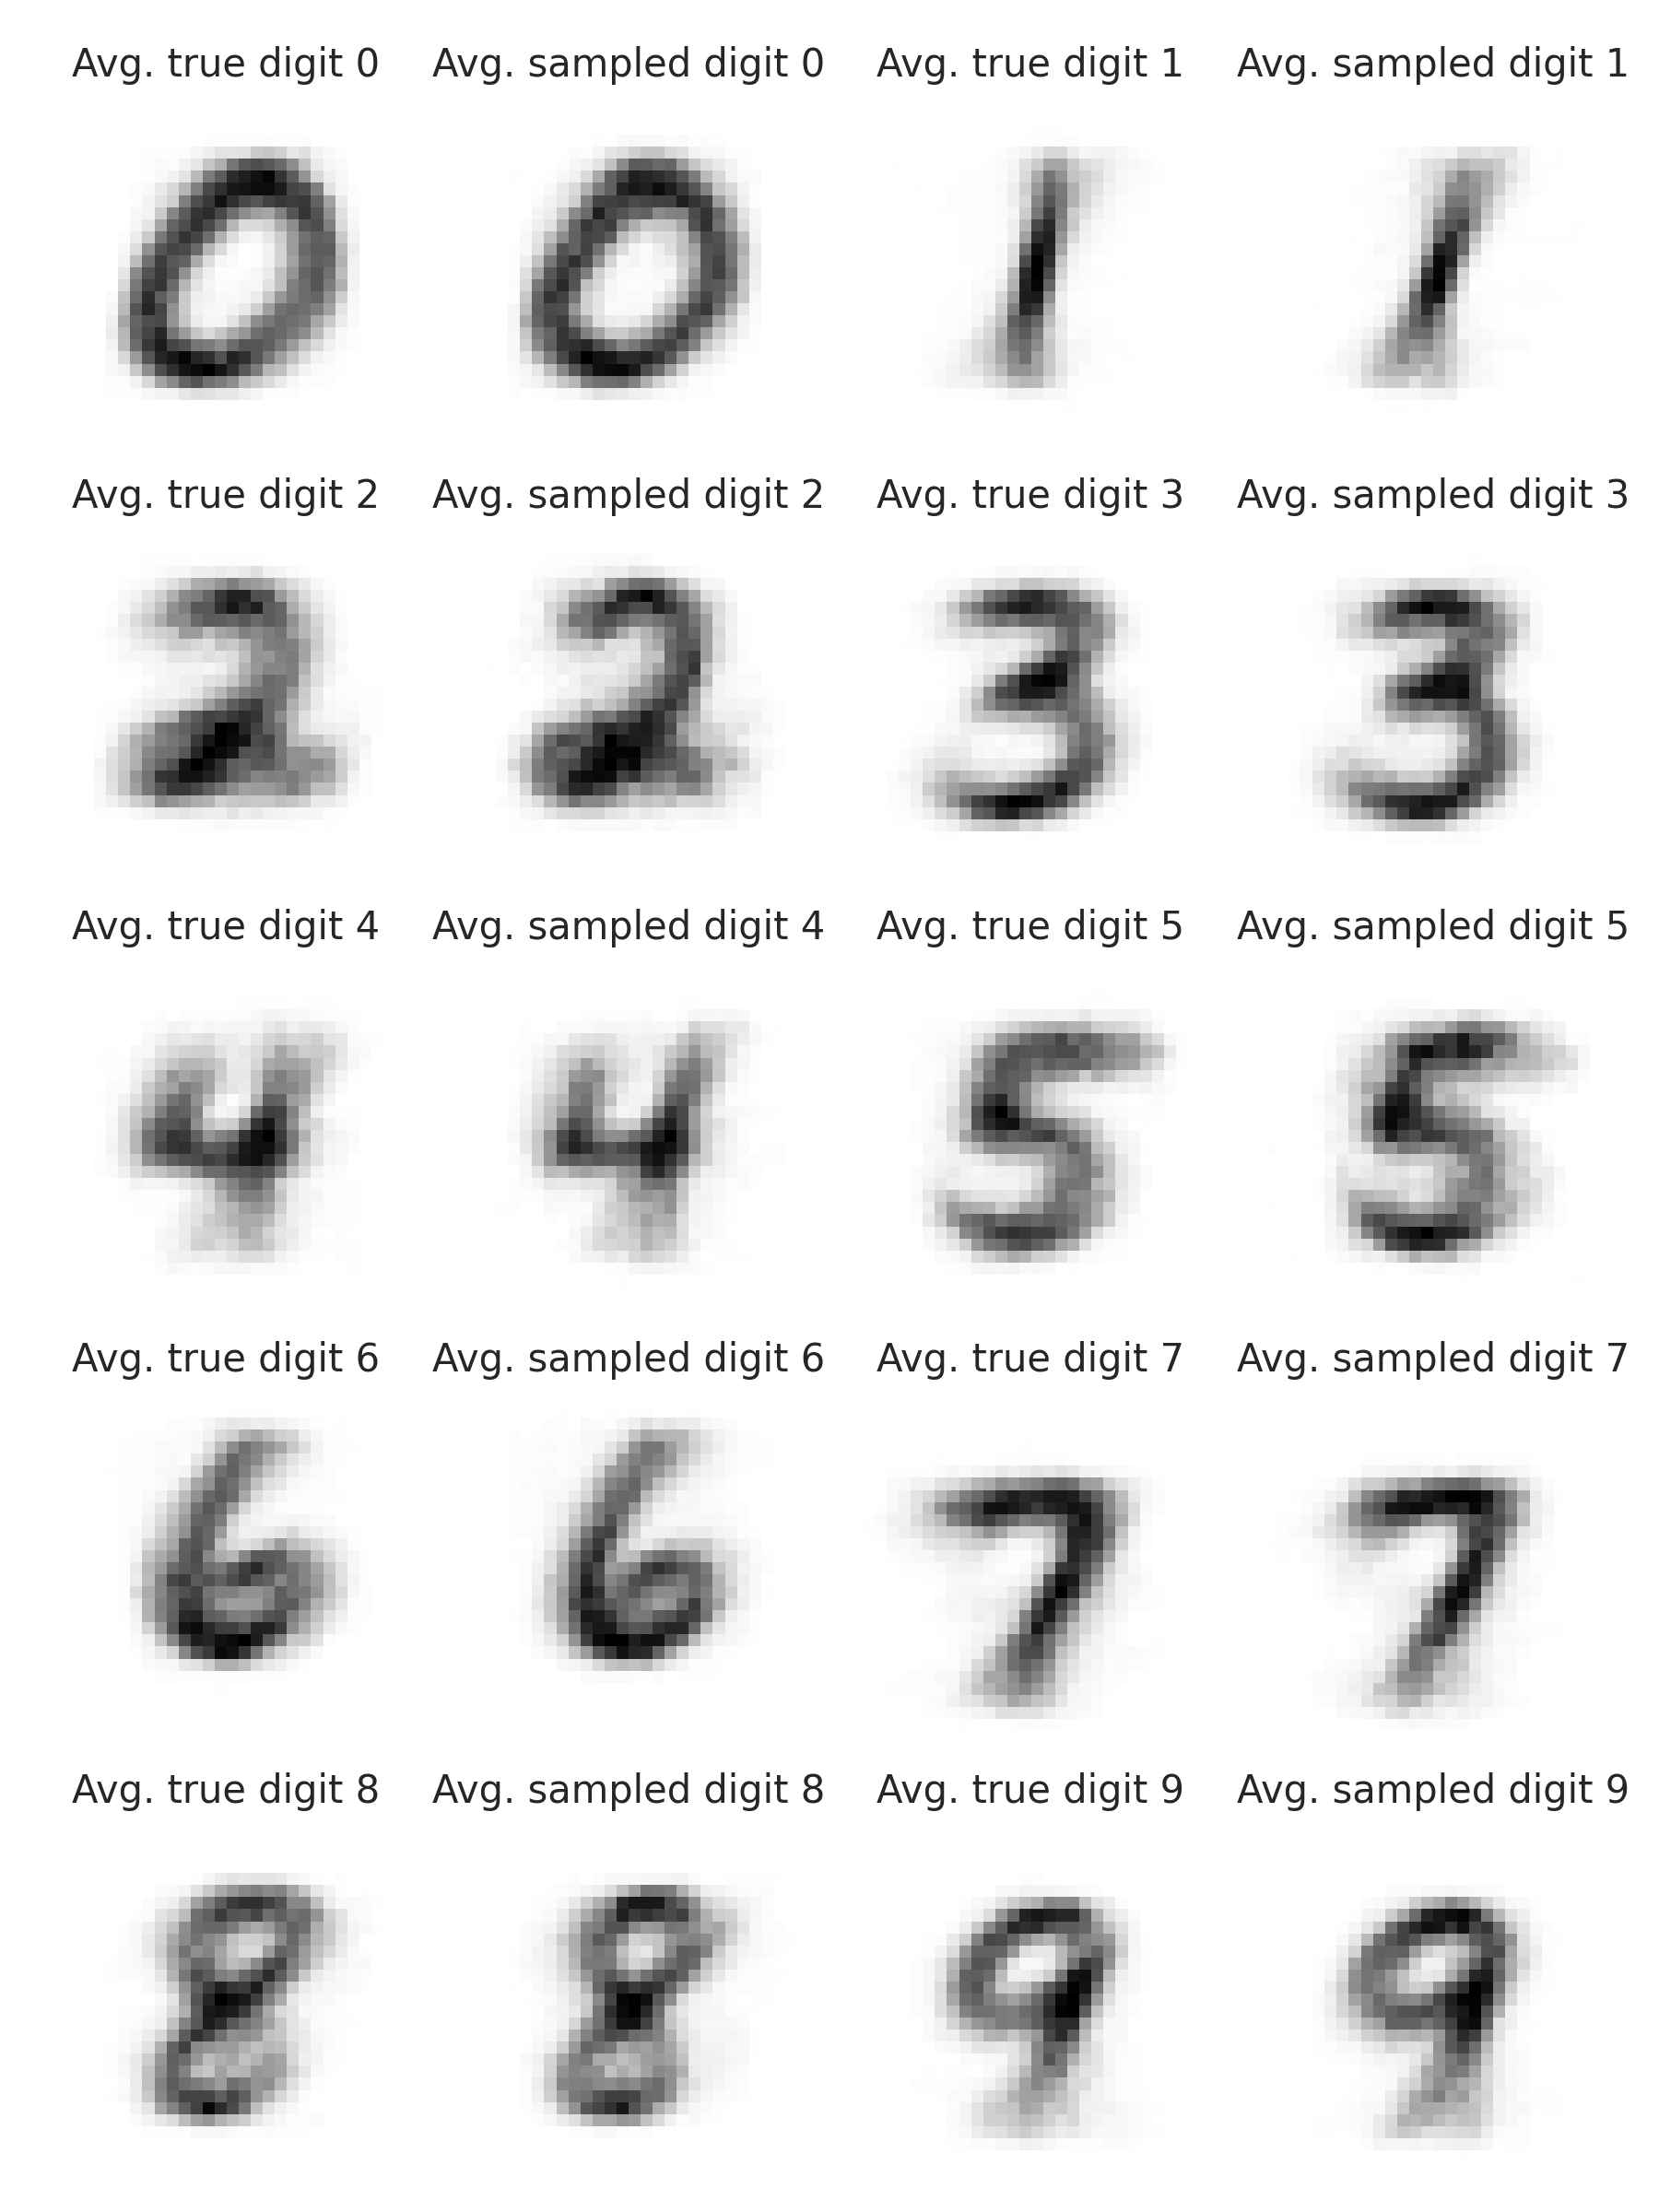
\includegraphics[width=0.5\textwidth]{images/bda_checks/mnist/BDA_model_sample_check.png}
    \caption{Average sampled digits from the held-out dataset are plotted next (left) to average sampled digits from the posterior predictive of the MNIST digit identity latent structure model (right).}
    \label{fig:bda_check_mnist_sample_plot}
\end{figure}

% MNIST posterior predictive checks
\begin{figure*}[h!]
    \centering
    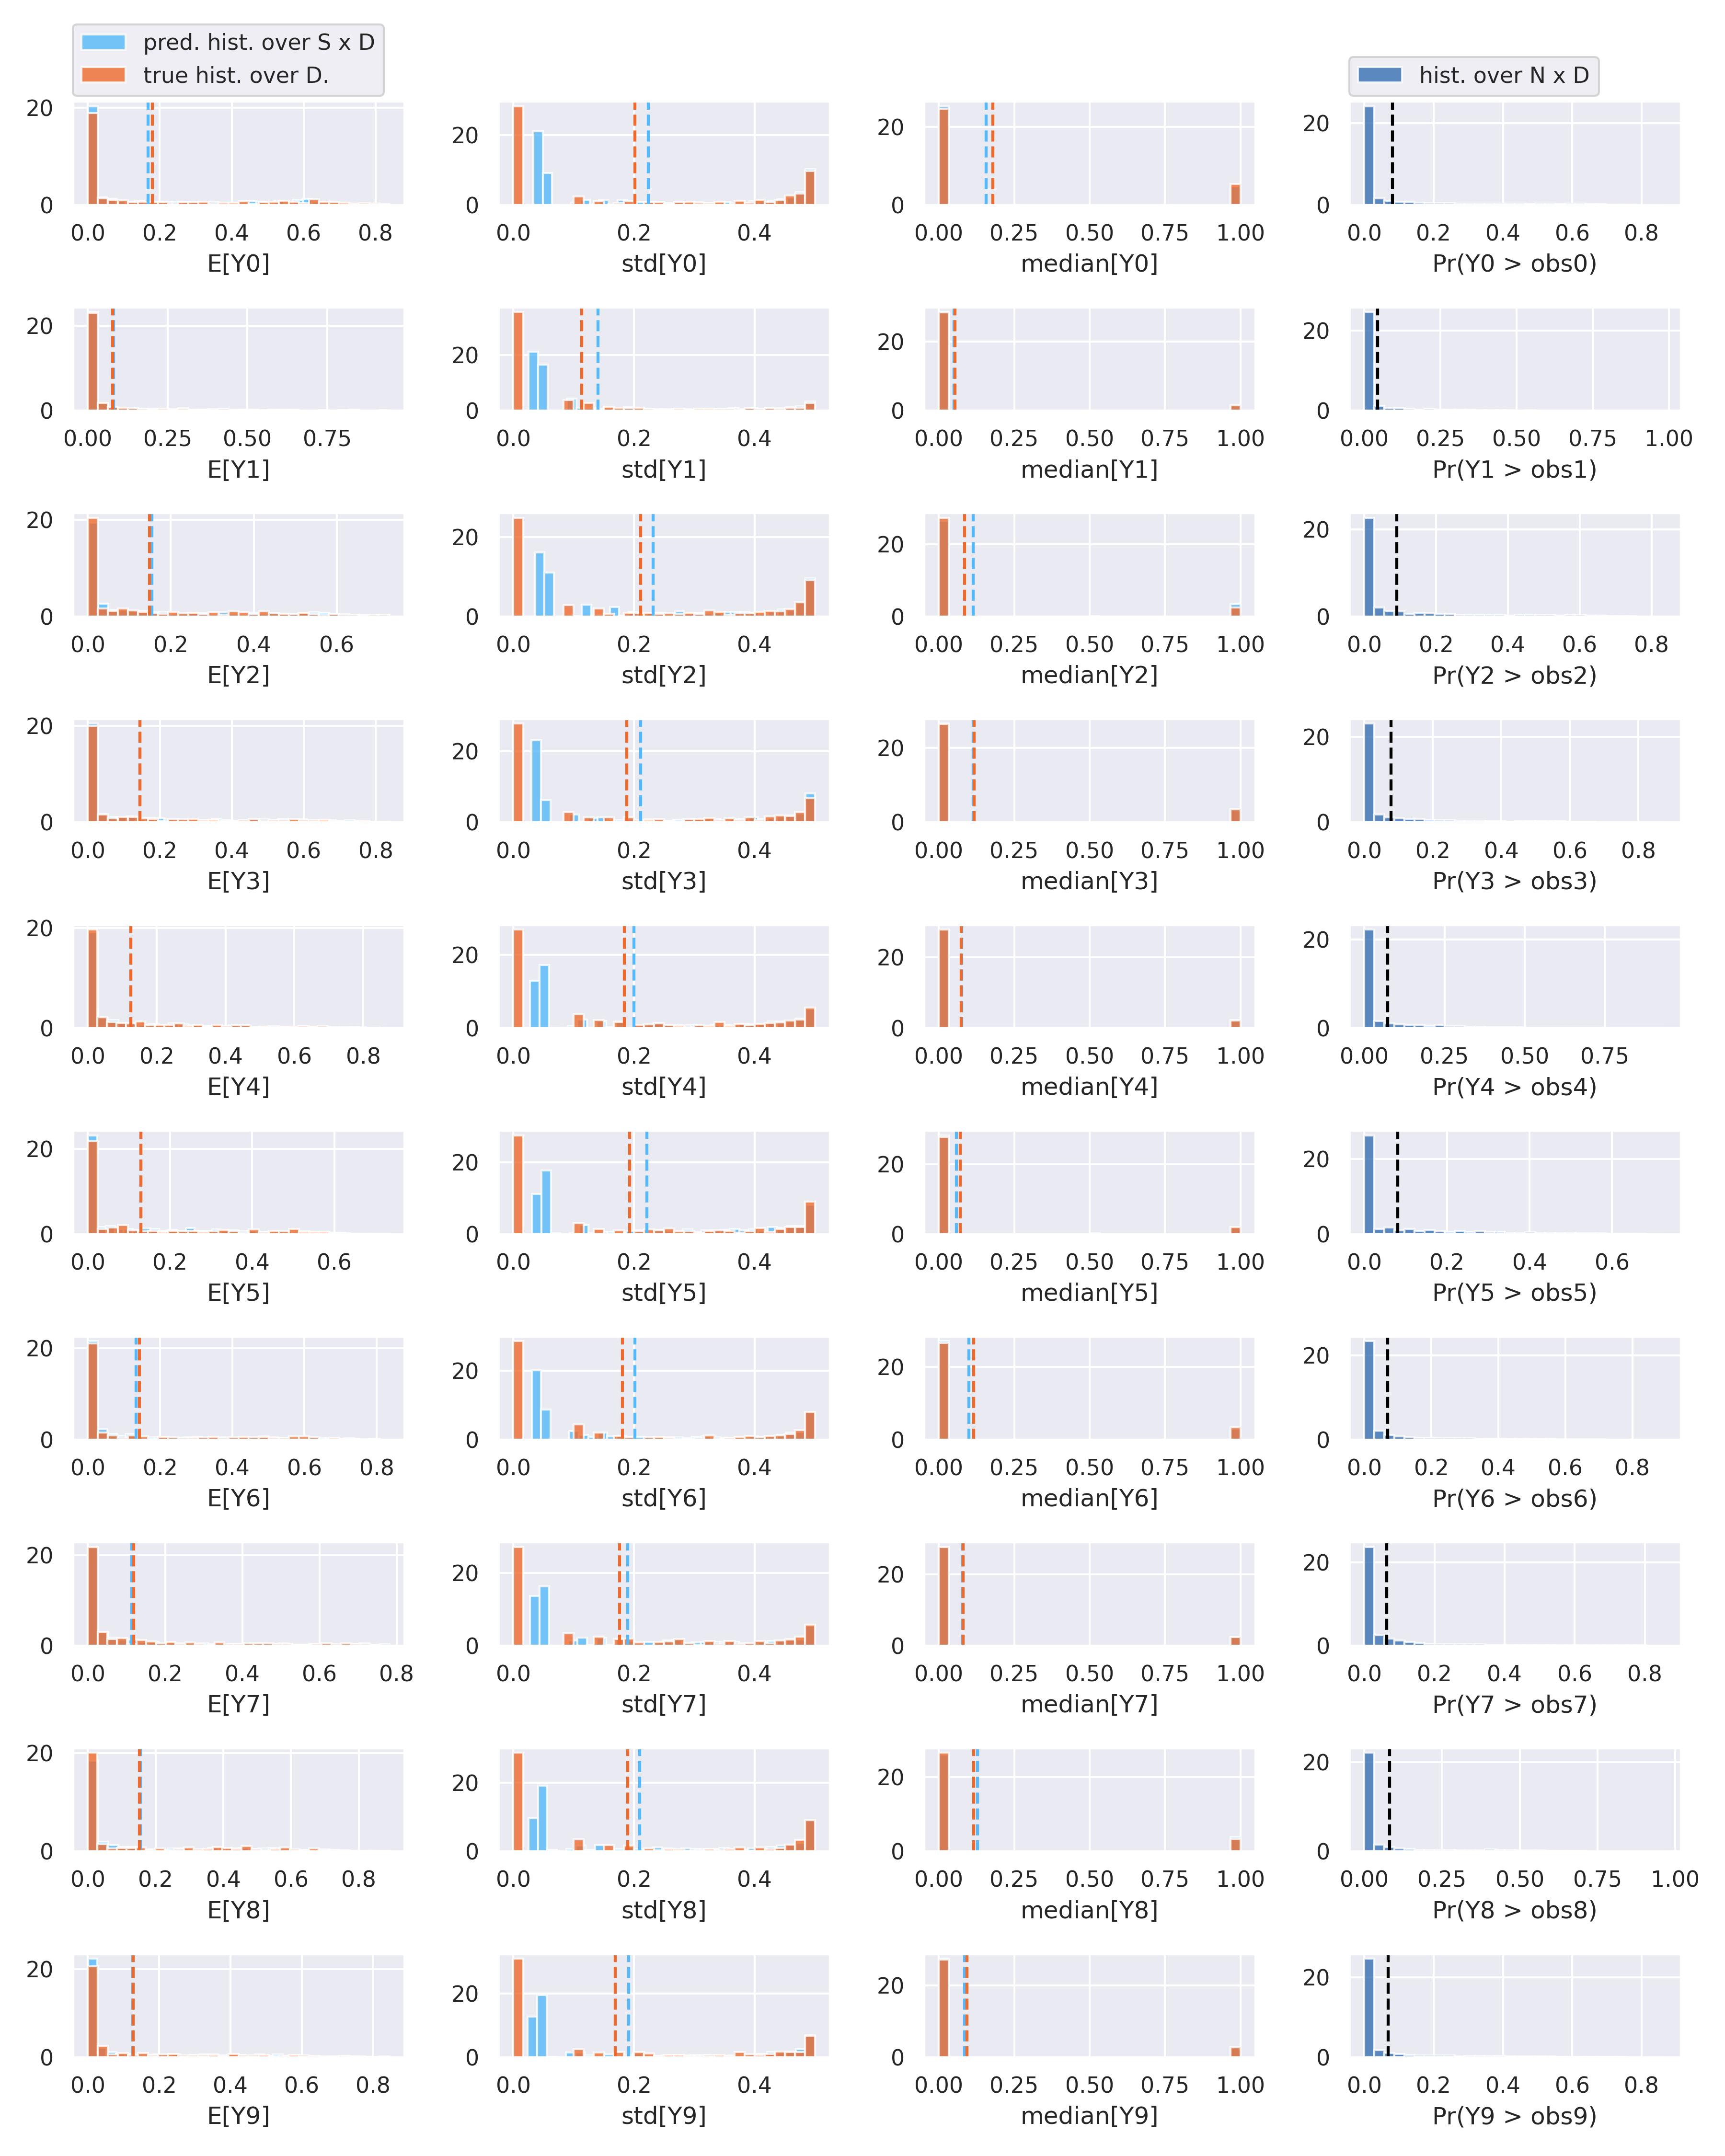
\includegraphics[width=\textwidth]{images/bda_checks/mnist/posterior_predictive_checks.png}
    \caption{Posterior predictive checks for the MNIST digit identity latent structure model fit to the data, row-wise organised per digit group. From left to right it shows histograms over the mean, the standard deviation, the median and the probability that a sampled pixel value from the posterior predictive exceeds that of a sampled pixel from held out observations.}
    \label{fig:bda_check_mnist_posterior_predictive_checks}
\end{figure*}

\subsubsection{PTB sequence length}

In Figure \ref{fig:ptb_data_model_length_distributions} histograms of the sampled lengths of the models trained on the Penn Treebank dataset are shown together with the true lengths. This is the raw data used for the sequence length latent structure model. Posterior predictive checks for this latent structure model fit on the held out data are shown in Figure \ref{fig:bda_check_ptb_seq_len_posterior_predictive_checks_1} and Figure  \ref{fig:bda_check_ptb_seq_len_posterior_predictive_checks_2}.

% Sequence length histograms
\begin{figure*}[!htb]
    \centering
    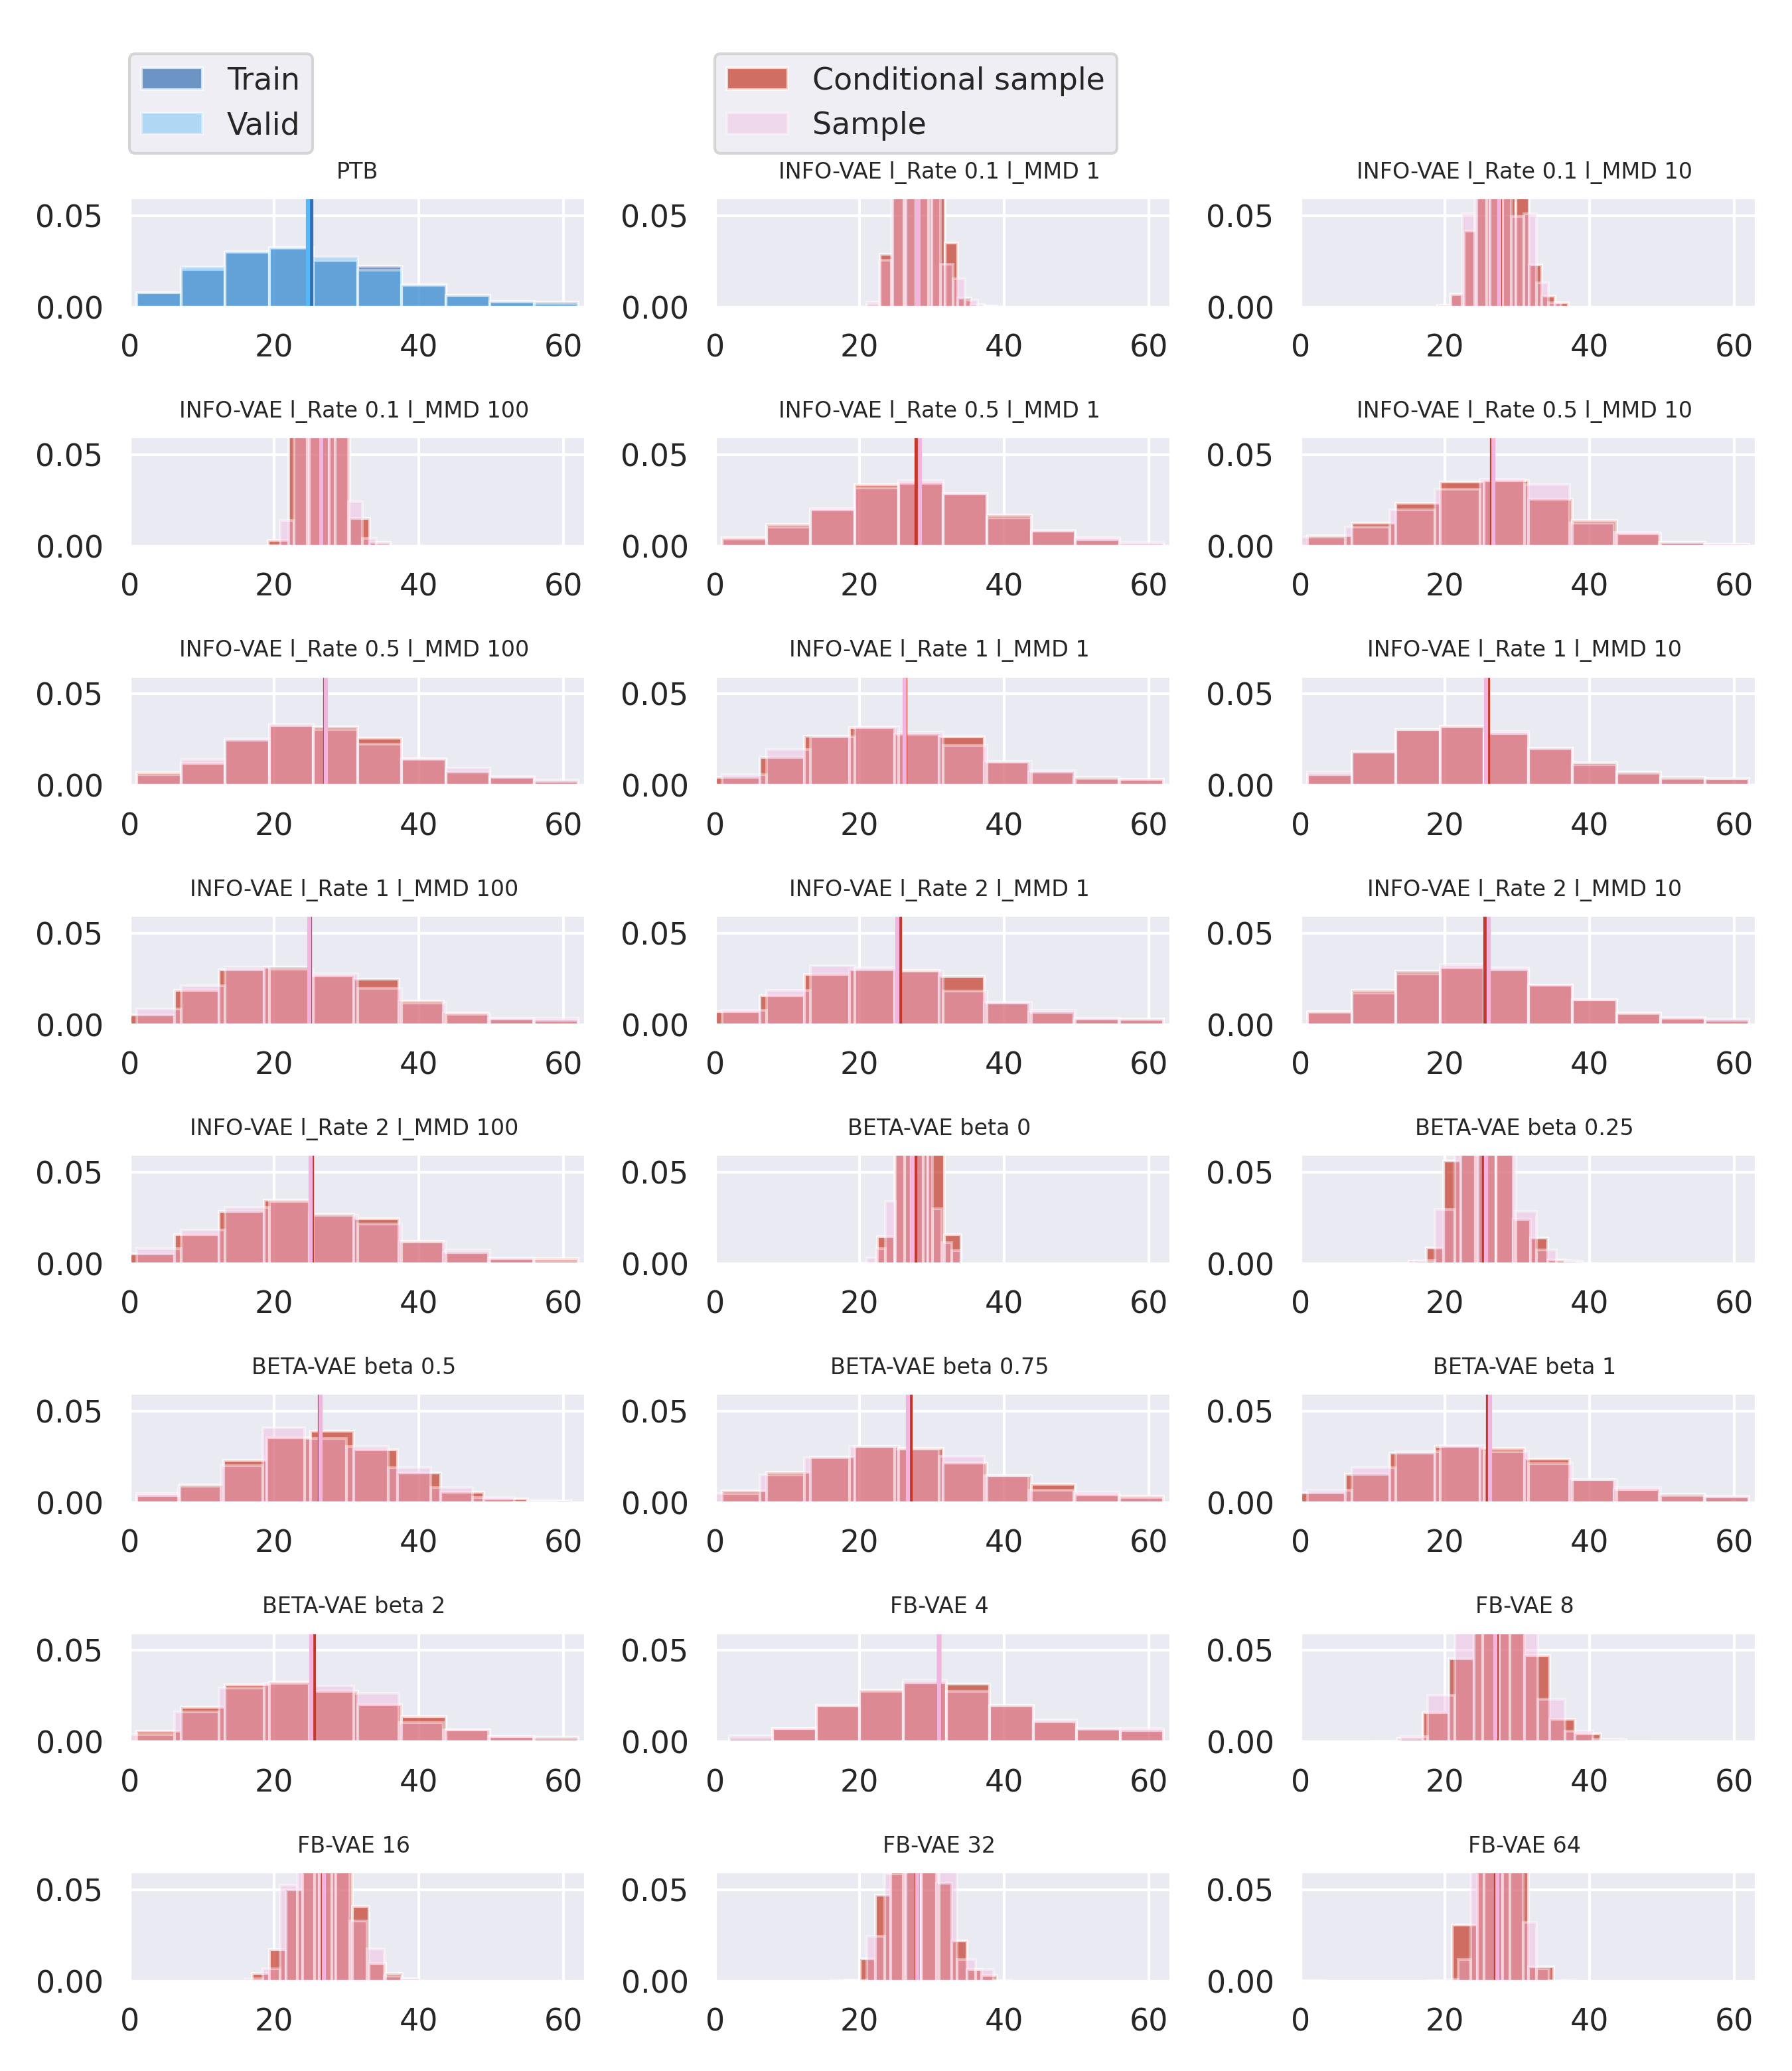
\includegraphics[width=0.7\textwidth]{images/bda_checks/pbt_seq_len/sequence_lengths_hists.png}
    \caption{Sequence length histograms of model samples (pink and red hues) and data samples (blue hues).}
    \label{fig:ptb_data_model_length_distributions}
\end{figure*}

% Posterior predictive checks sequence length model
\begin{figure*}[!htb]
    \centering
    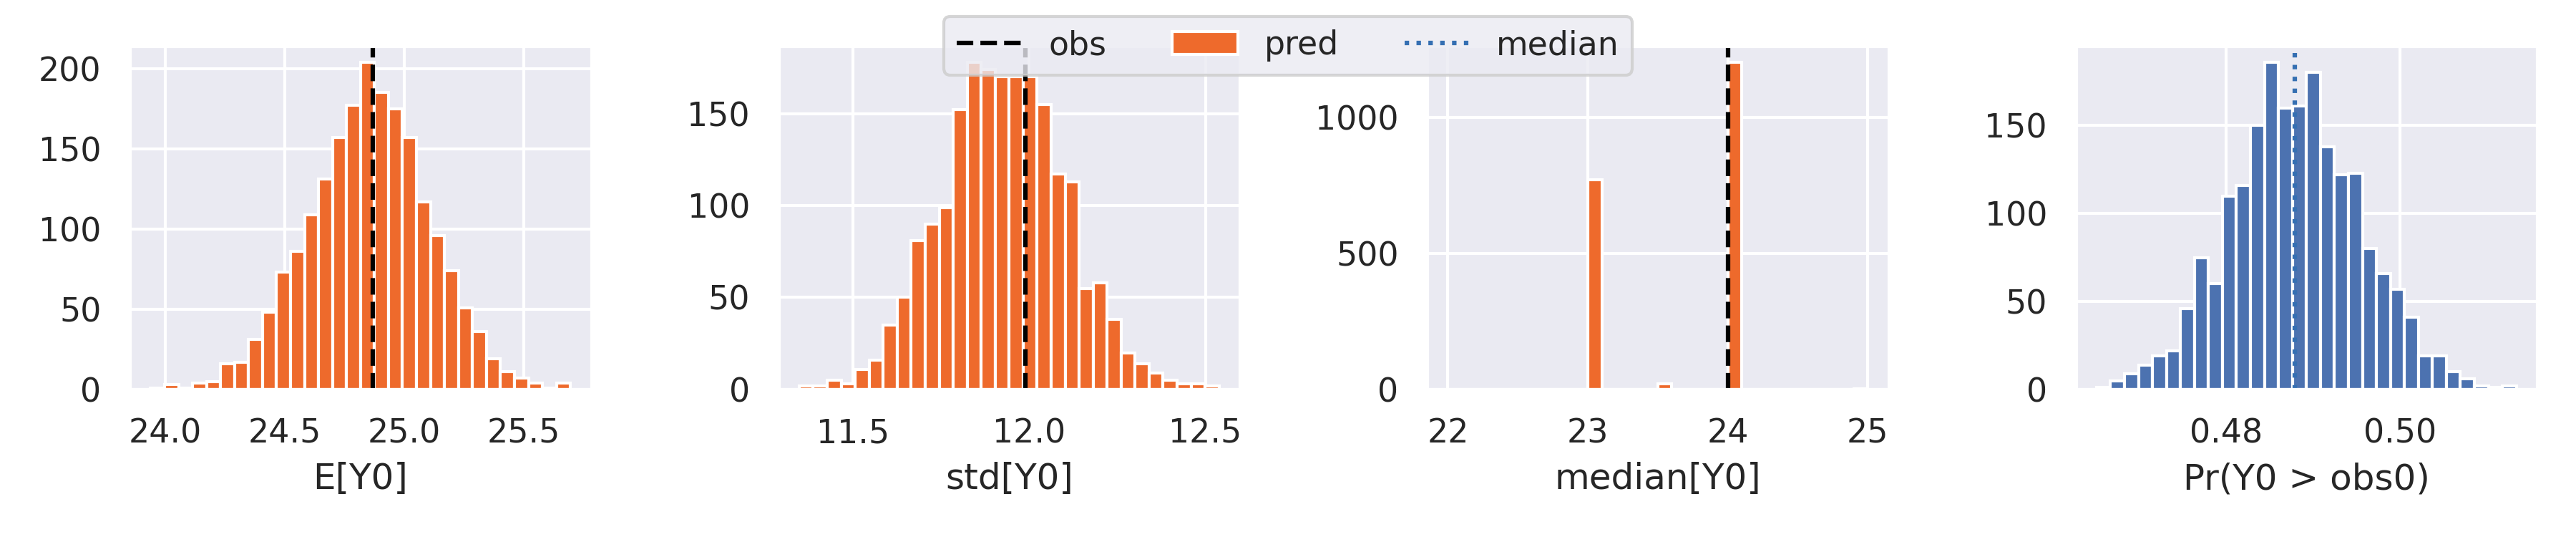
\includegraphics[width=\textwidth]{images/bda_checks/pbt_seq_len/posterior_predictive_check_pvals.png}
    \caption{Posterior predictive checks for the sequence length latent structure model. From left to right it shows histograms over the mean, the standard deviation, the median and the probability that a sampled length value from the posterior predictive exceeds that of a sampled length from held out observations.}
    \label{fig:bda_check_ptb_seq_len_posterior_predictive_checks_1}
\end{figure*}

% True and posterior sampled length distribution
\begin{figure*}[!htb]
    \centering
    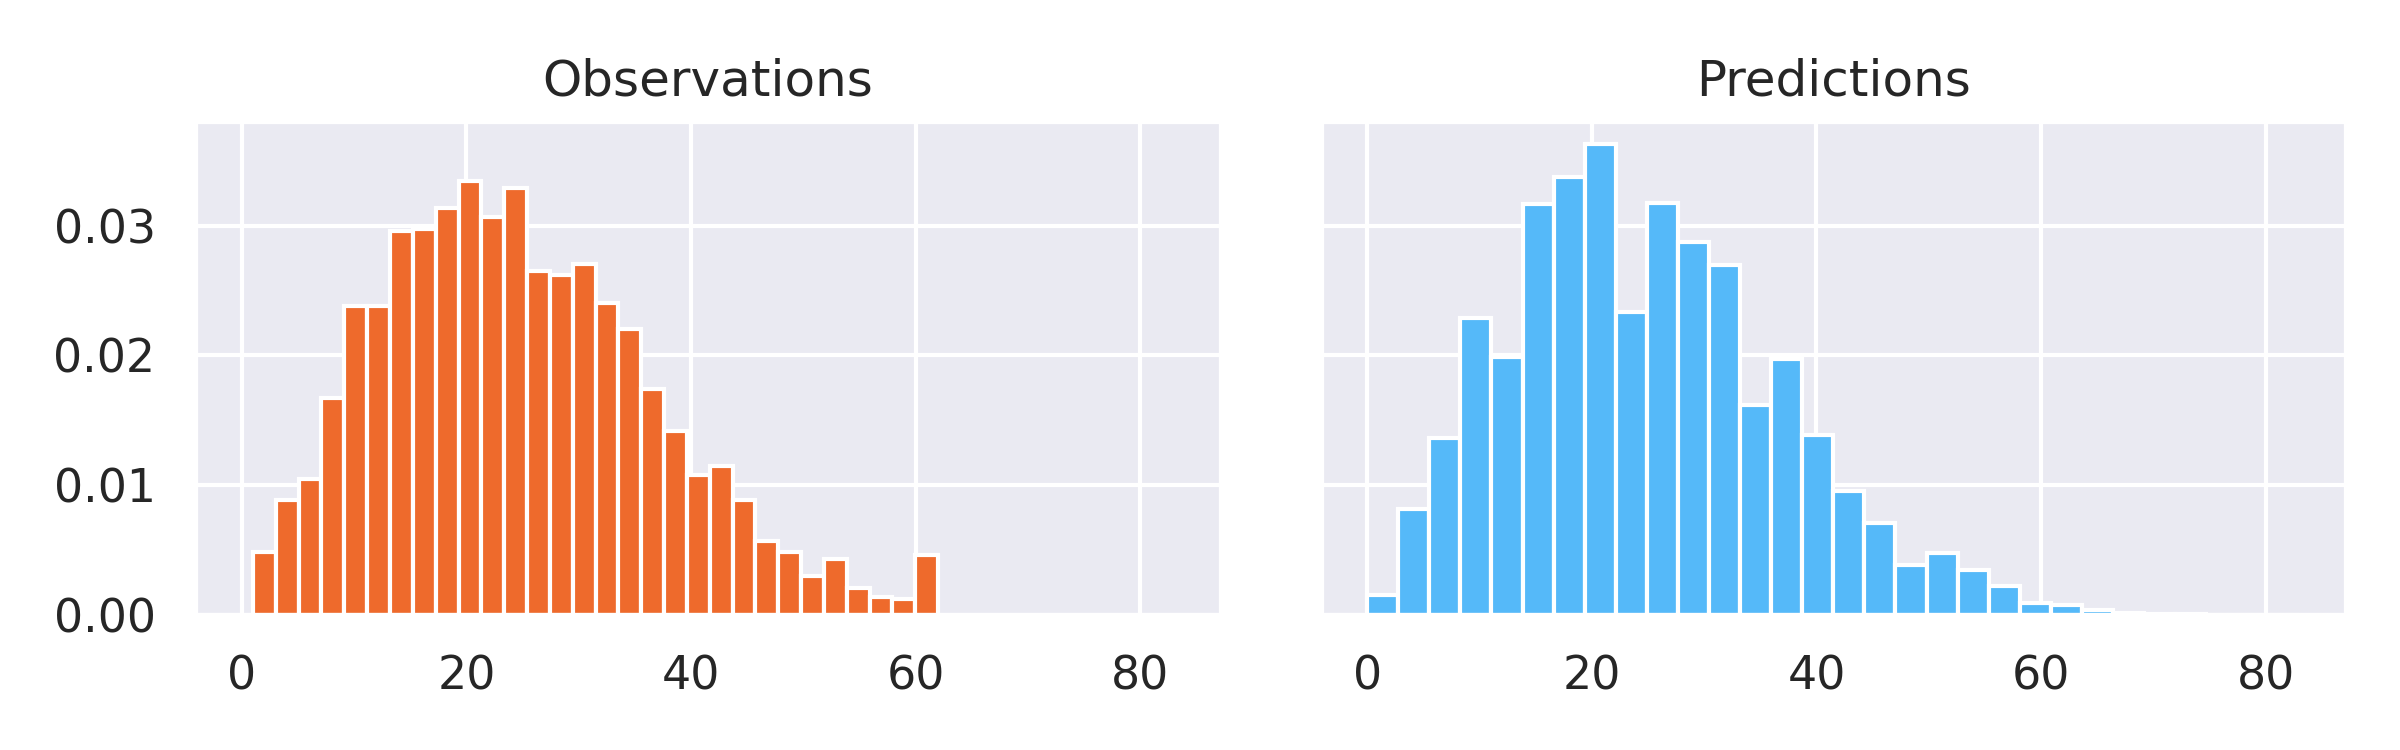
\includegraphics[width=0.6\textwidth]{images/bda_checks/pbt_seq_len/posterior_predictive_check_preds.png}
    \caption{A histogram of sampled lengths from the held out Penn Treebank dataset (left) next to sampled lengths from the posterior predictive of the sequence length latent structure model (right).}
    \label{fig:bda_check_ptb_seq_len_posterior_predictive_checks_2}
\end{figure*}

\subsubsection{PTB topics}

% LDA hyperparameter experiment
\begin{figure*}[!htb]
    \centering
    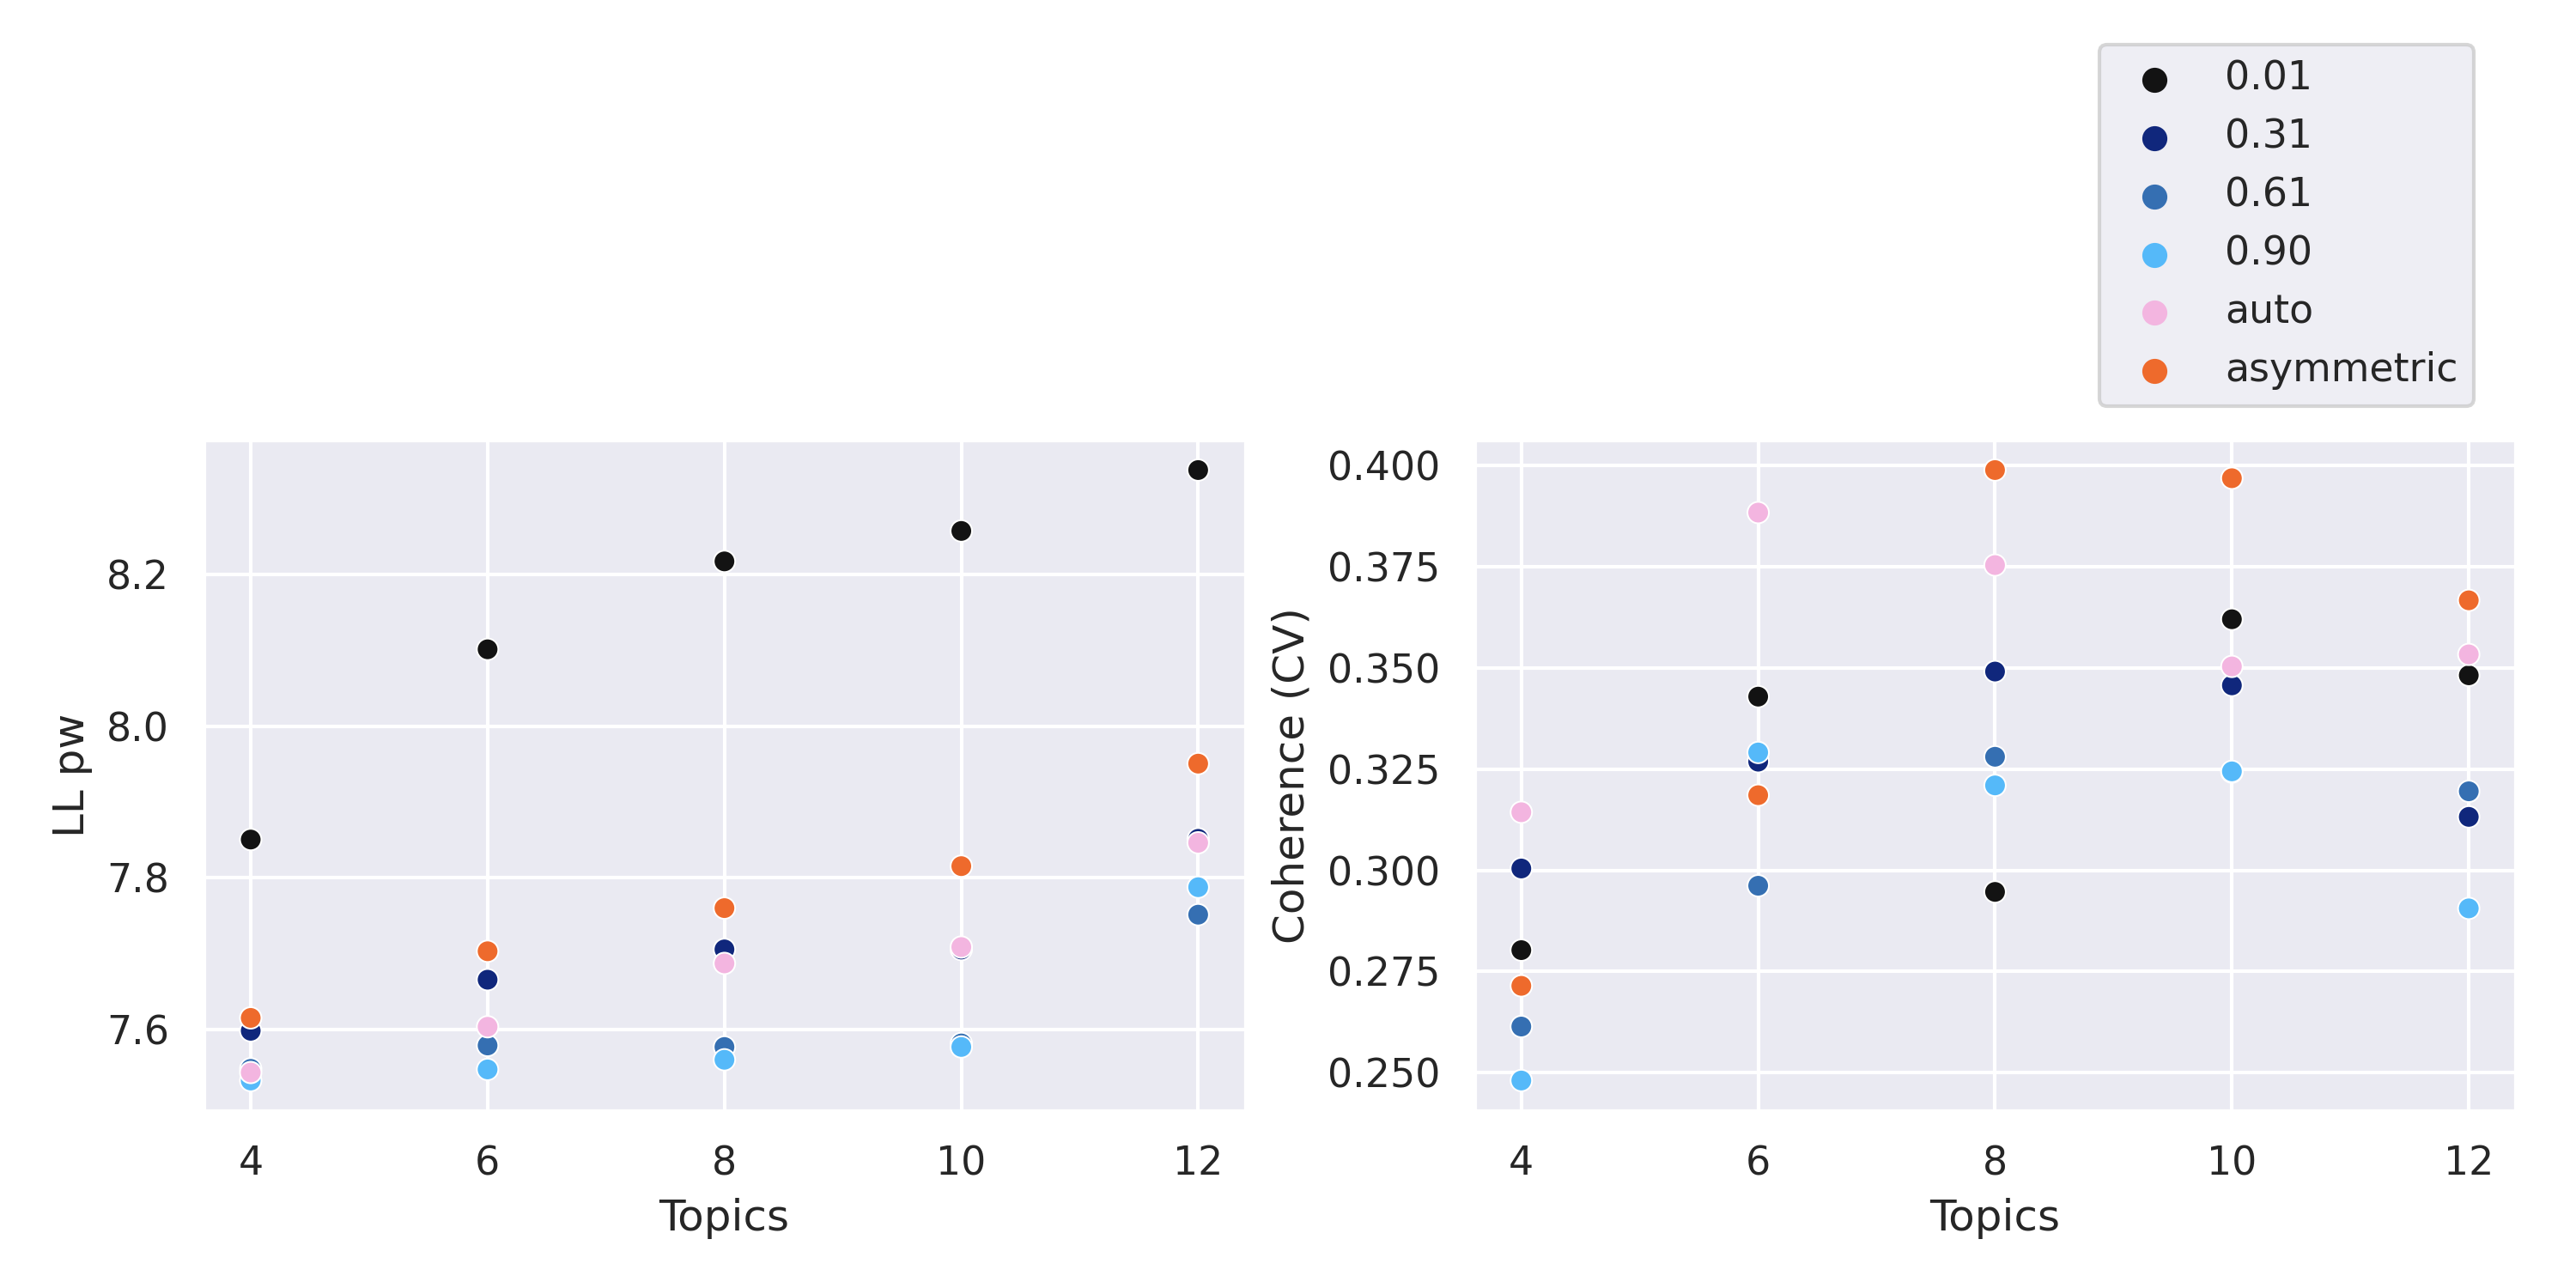
\includegraphics[width=0.75\textwidth]{images/bda_checks/ptb_topics/LDA_tune_results.png}
    \caption{The per-token log likelihood bound and a sliding window topic coherence for different number of topics and different values for \texttt{alpha}.}
    \label{fig:bda_checks_lda_hp_tuning}
\end{figure*}

% LDA word freq plot
\begin{figure*}[!htb]
    \centering
    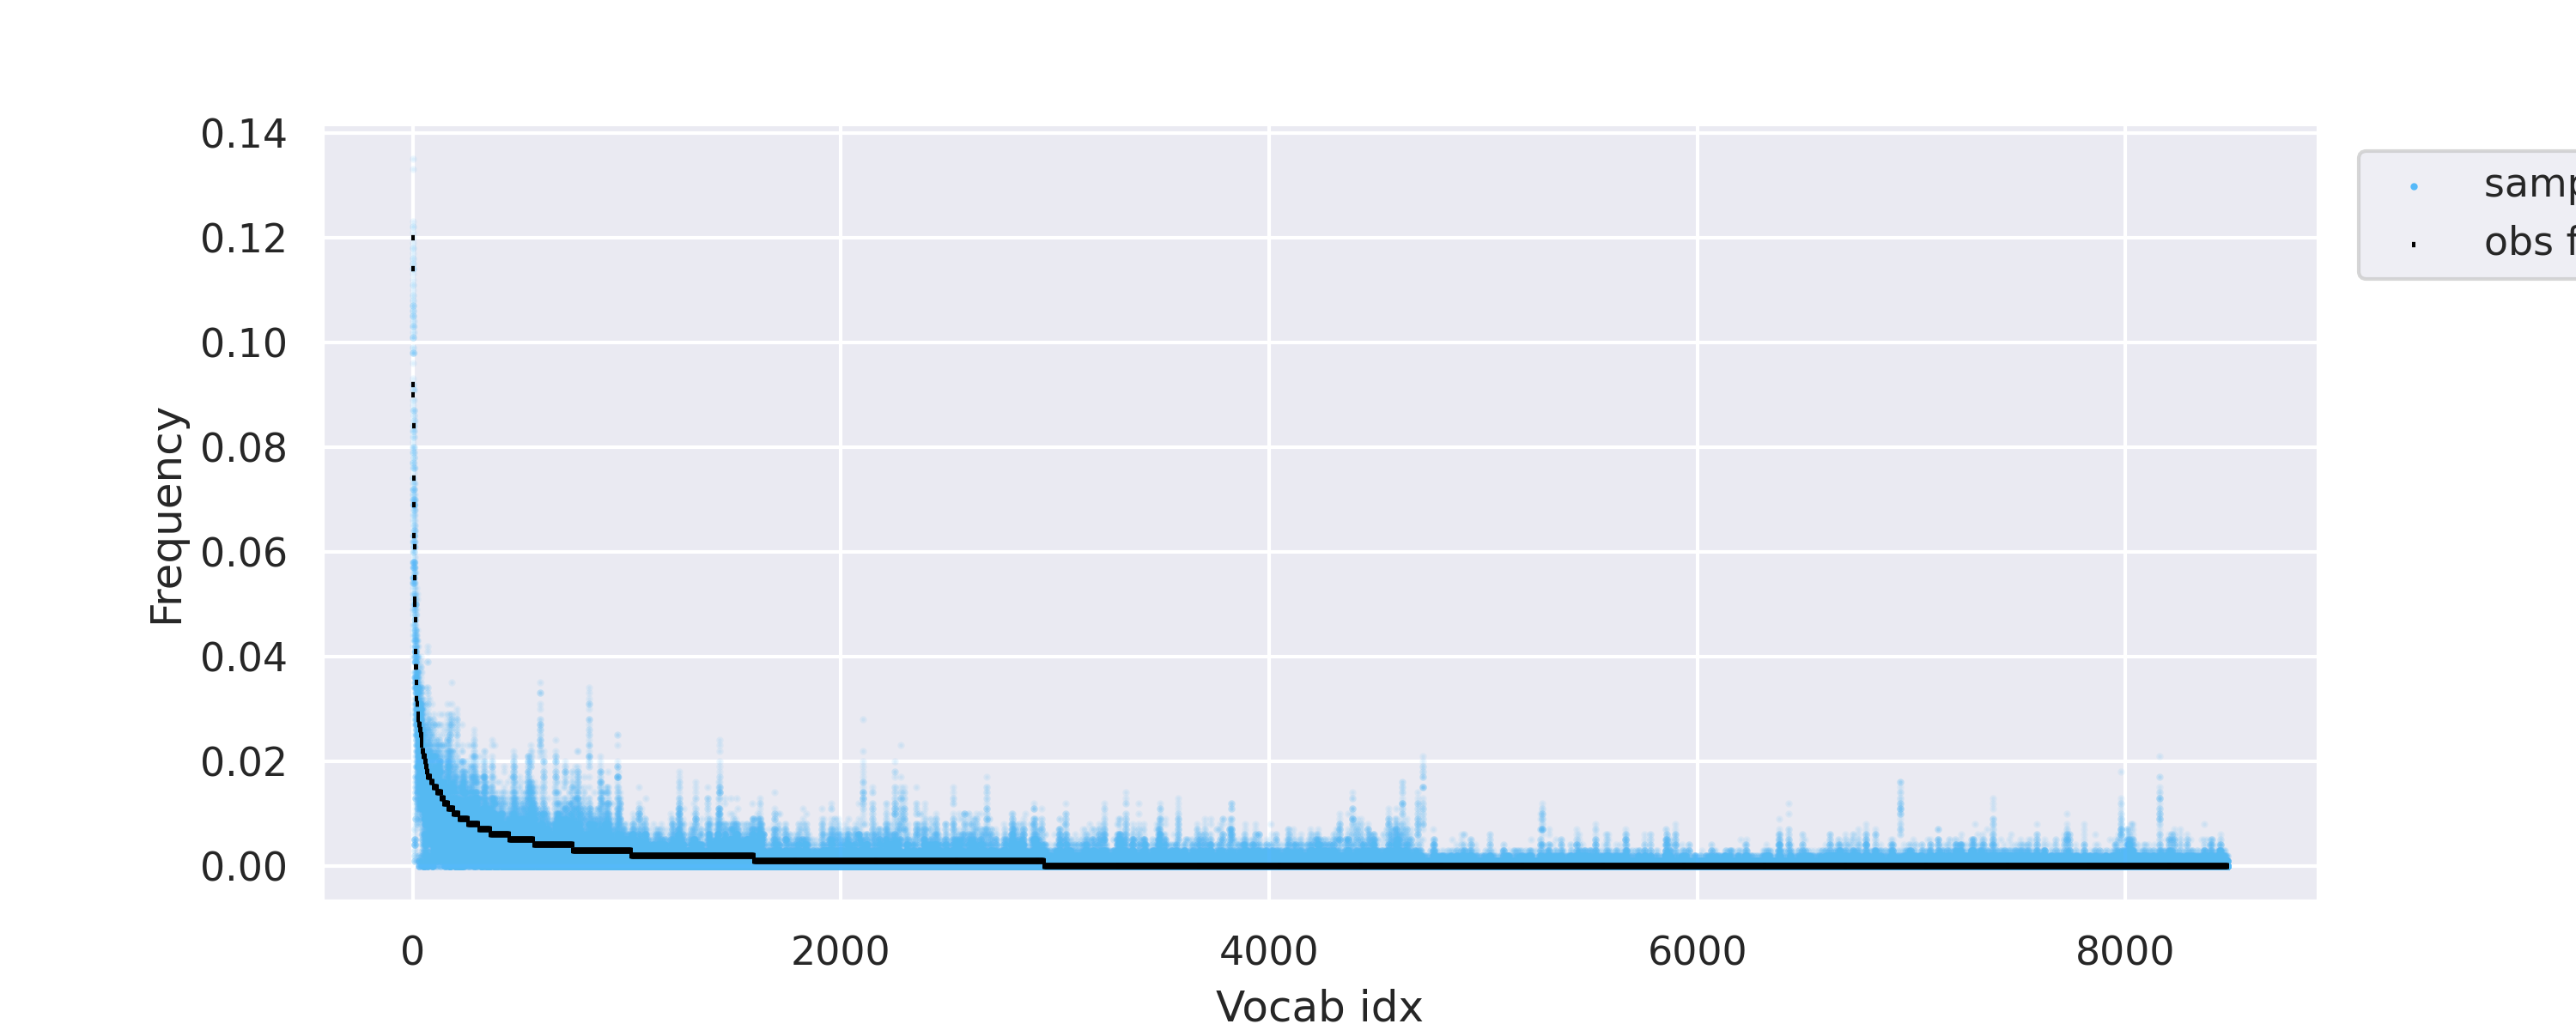
\includegraphics[width=0.8\textwidth]{images/bda_checks/ptb_topics/lda_word_dist_check.png}
    \caption{True sorted token frequencies of the Penn Treebank data set plotted against re-sampled sorted token frequencies sampled from the fitted LDA model.}
    \label{fig:bda_checks_lda_word_freqs}
\end{figure*}

% LDA top tokens per topic table
\begin{table*}[!htb]
    \centering
    \scriptsize
    \begin{tabular}{rllllllllll}
\toprule
 Topic &  Token 0 & Token 1 &     Token 2 &    Token 3 &    Token 4 &    Token 5 &   Token 6 &   Token 7 &         Token 8 &    Token 9 \\
\midrule
     0 &   market &   stock &       price &    trading &   investor &        day &    trader &    future &           index &        buy \\
     1 &       mr &     say &         big &        dow &      jones &  dow\_jones &       one &     point &           world &      going \\
     2 &     test &      mr &      cancer &      house &  treatment &   director &     state &   federal &         whether &     senate \\
     3 &  million &   share &        year &    billion &       sale &    earlier &   quarter &   company &            rose &      month \\
     4 &  company &     new &  laboratory &  operation &    billion &       corp &     calif &      loan &             los &    deficit \\
     5 &     bond &    rate &        year &     dollar &     market &      franc &      bank &  interest &         billion &      yield \\
     6 &  company &     inc &       third &       corp &  president &  executive &     chief &        co &   third\_quarter &     unilab \\
     7 &      new &    york &    new\_york &      stock &   exchange &      month &    closed &   trading &  stock\_exchange &  yesterday \\
     8 &     next &    data &     control &     export &      would &    company &  spending &      year &        computer &     friday \\
     9 &       mr &     say &        year &      could &      buyer &    central &      drug &       old &            time &      would \\
\bottomrule
\end{tabular}
    \caption{The top 10 tokens per topic as identified by the LDA topic model.}
    \label{tab:lda_topic_words}
\end{table*}


To choose the hyperparameters of the LDA topic model that is fit to the Penn Treebank data, we perform a hyperparameter experiment. To this end, we compute the per-token log likelihood bound and a sliding window topic coherence score (Gensim's \texttt{c\_v}), using the held-out Penn Treebank data. Based on these results (visualised in Figure \ref{fig:bda_checks_lda_hp_tuning}) we set \texttt{alpha} to 0.01 and set the number of topics to 10. Figures \ref{fig:bda_checks_lda_word_freqs} shows an additional check to assess goodness of fit for the LDA model given these hyperparameters. % removed the other check it looks strange?




% LDA word freq error hist. <- I am not sure about this plot
% \begin{figure}
%     \centering
%     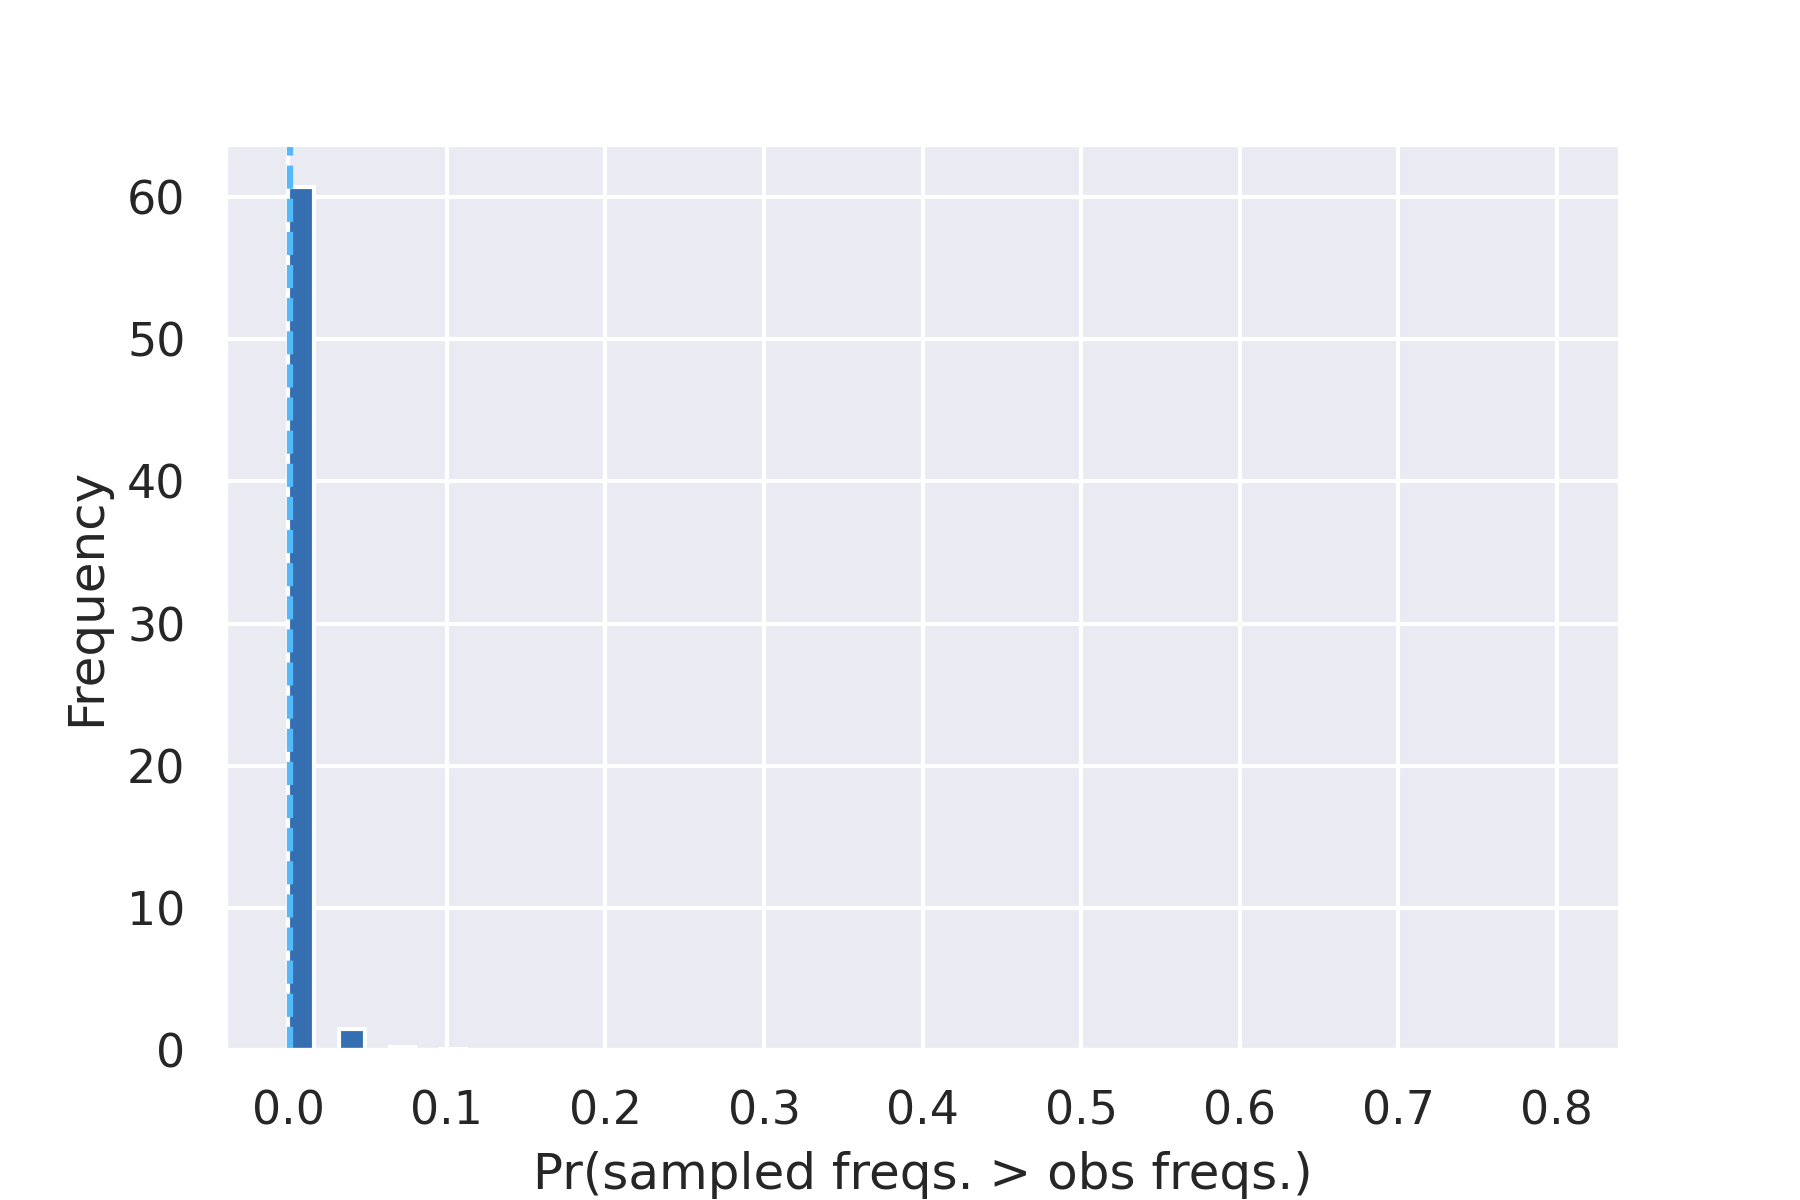
\includegraphics[width=0.35\textwidth]{images/bda_checks/ptb_topics/LDA_post_check_word_dist.png}
%     % \caption{A histogram of probabilities the LDA re-sampled token frequency exceeds the true token frequency.}
%     \caption{Posterior predictive check for LDA.}
%     \label{fig:bda_checks_lda_error_prob}
% \end{figure}




\subsubsection{Latent space}\label{app:latent-space}

In Figure \ref{fig:latent-component-plots} we plot the average posterior component sample for the latent analysis models.

\begin{figure*}[!htb]
    \centering
    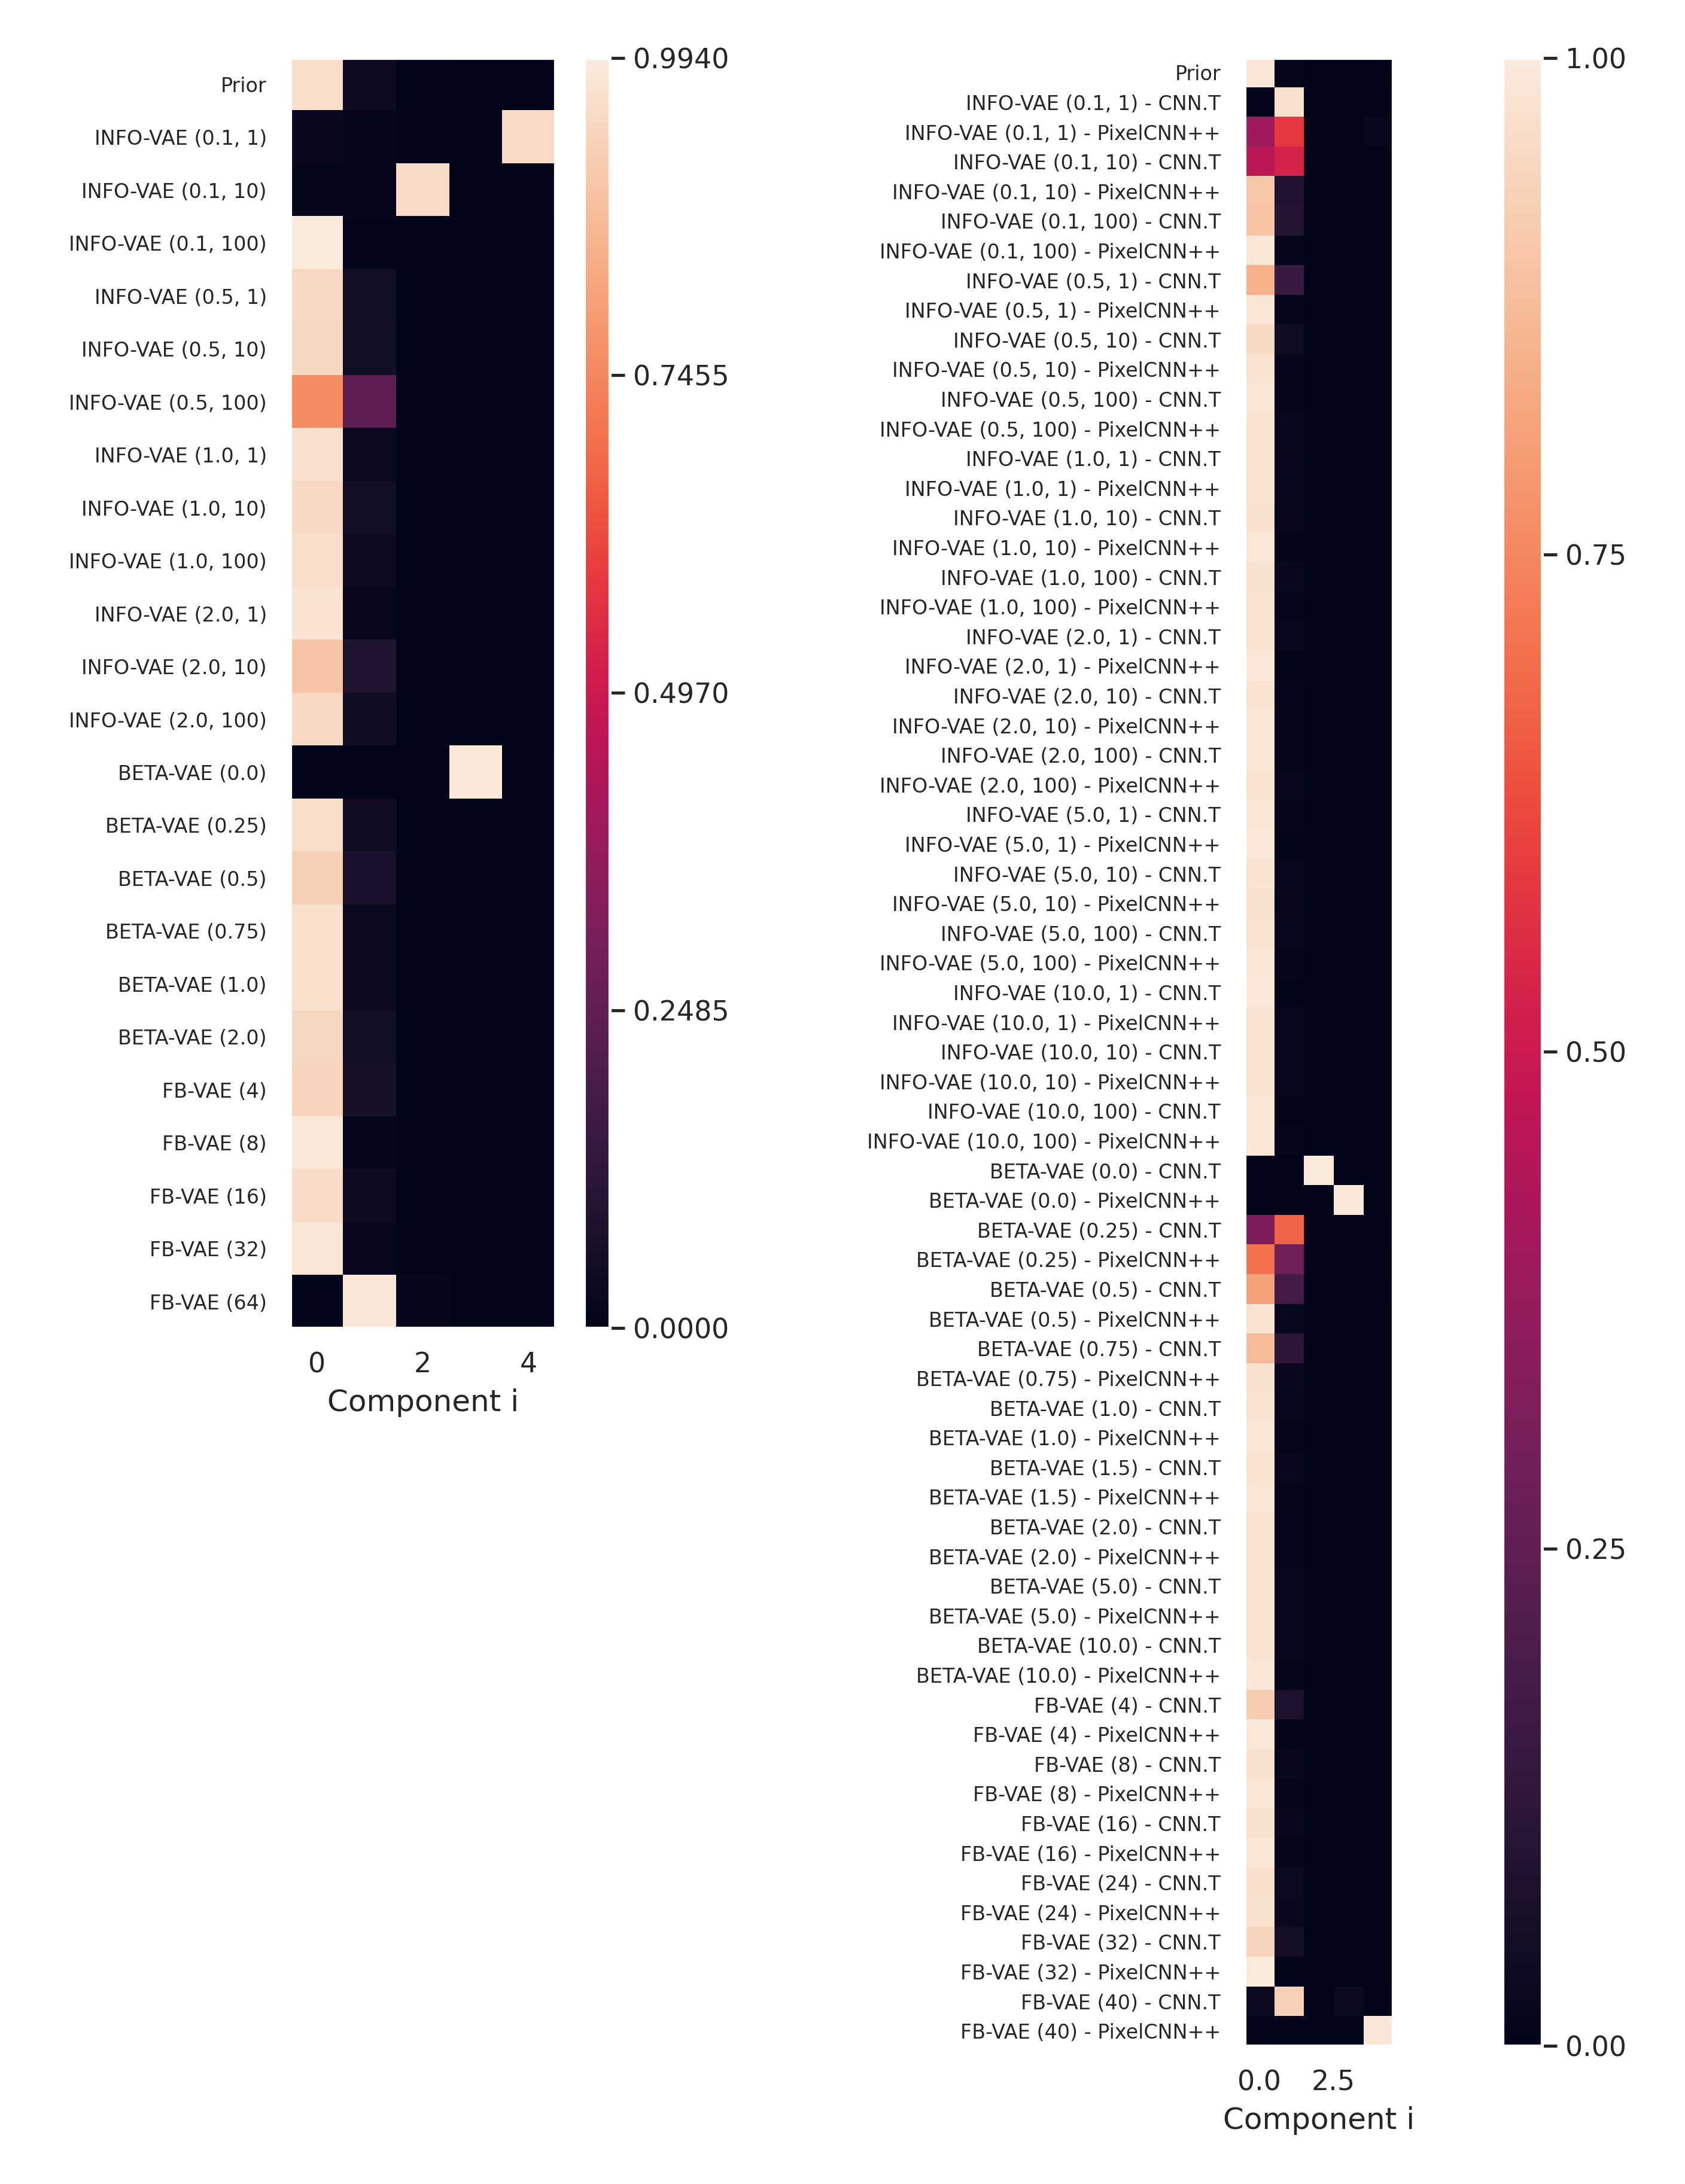
\includegraphics[width=0.8\textwidth]{images/latent-component-plots-06.png}
    \caption{Sampled components from the posterior of the latent analysis models for all experiment groups and the control (data group). The left column shows the PTB experiments, right the MNIST experiments.}
    \label{fig:latent-component-plots}
\end{figure*}

\subsection{Full experimental results lppd statistics}

Full experimental results for the three type of statistics measured under the three latent structure models can be found in Figures \ref{fig:mnist_surprisal_dist}, \ref{fig:ptb_seq_len_surprisal_dist} and \ref{fig:ptb_lda_topics_surprisal_dist}.

% MNIST surprisal distributions
\begin{figure*}[!htb]
    \centering
    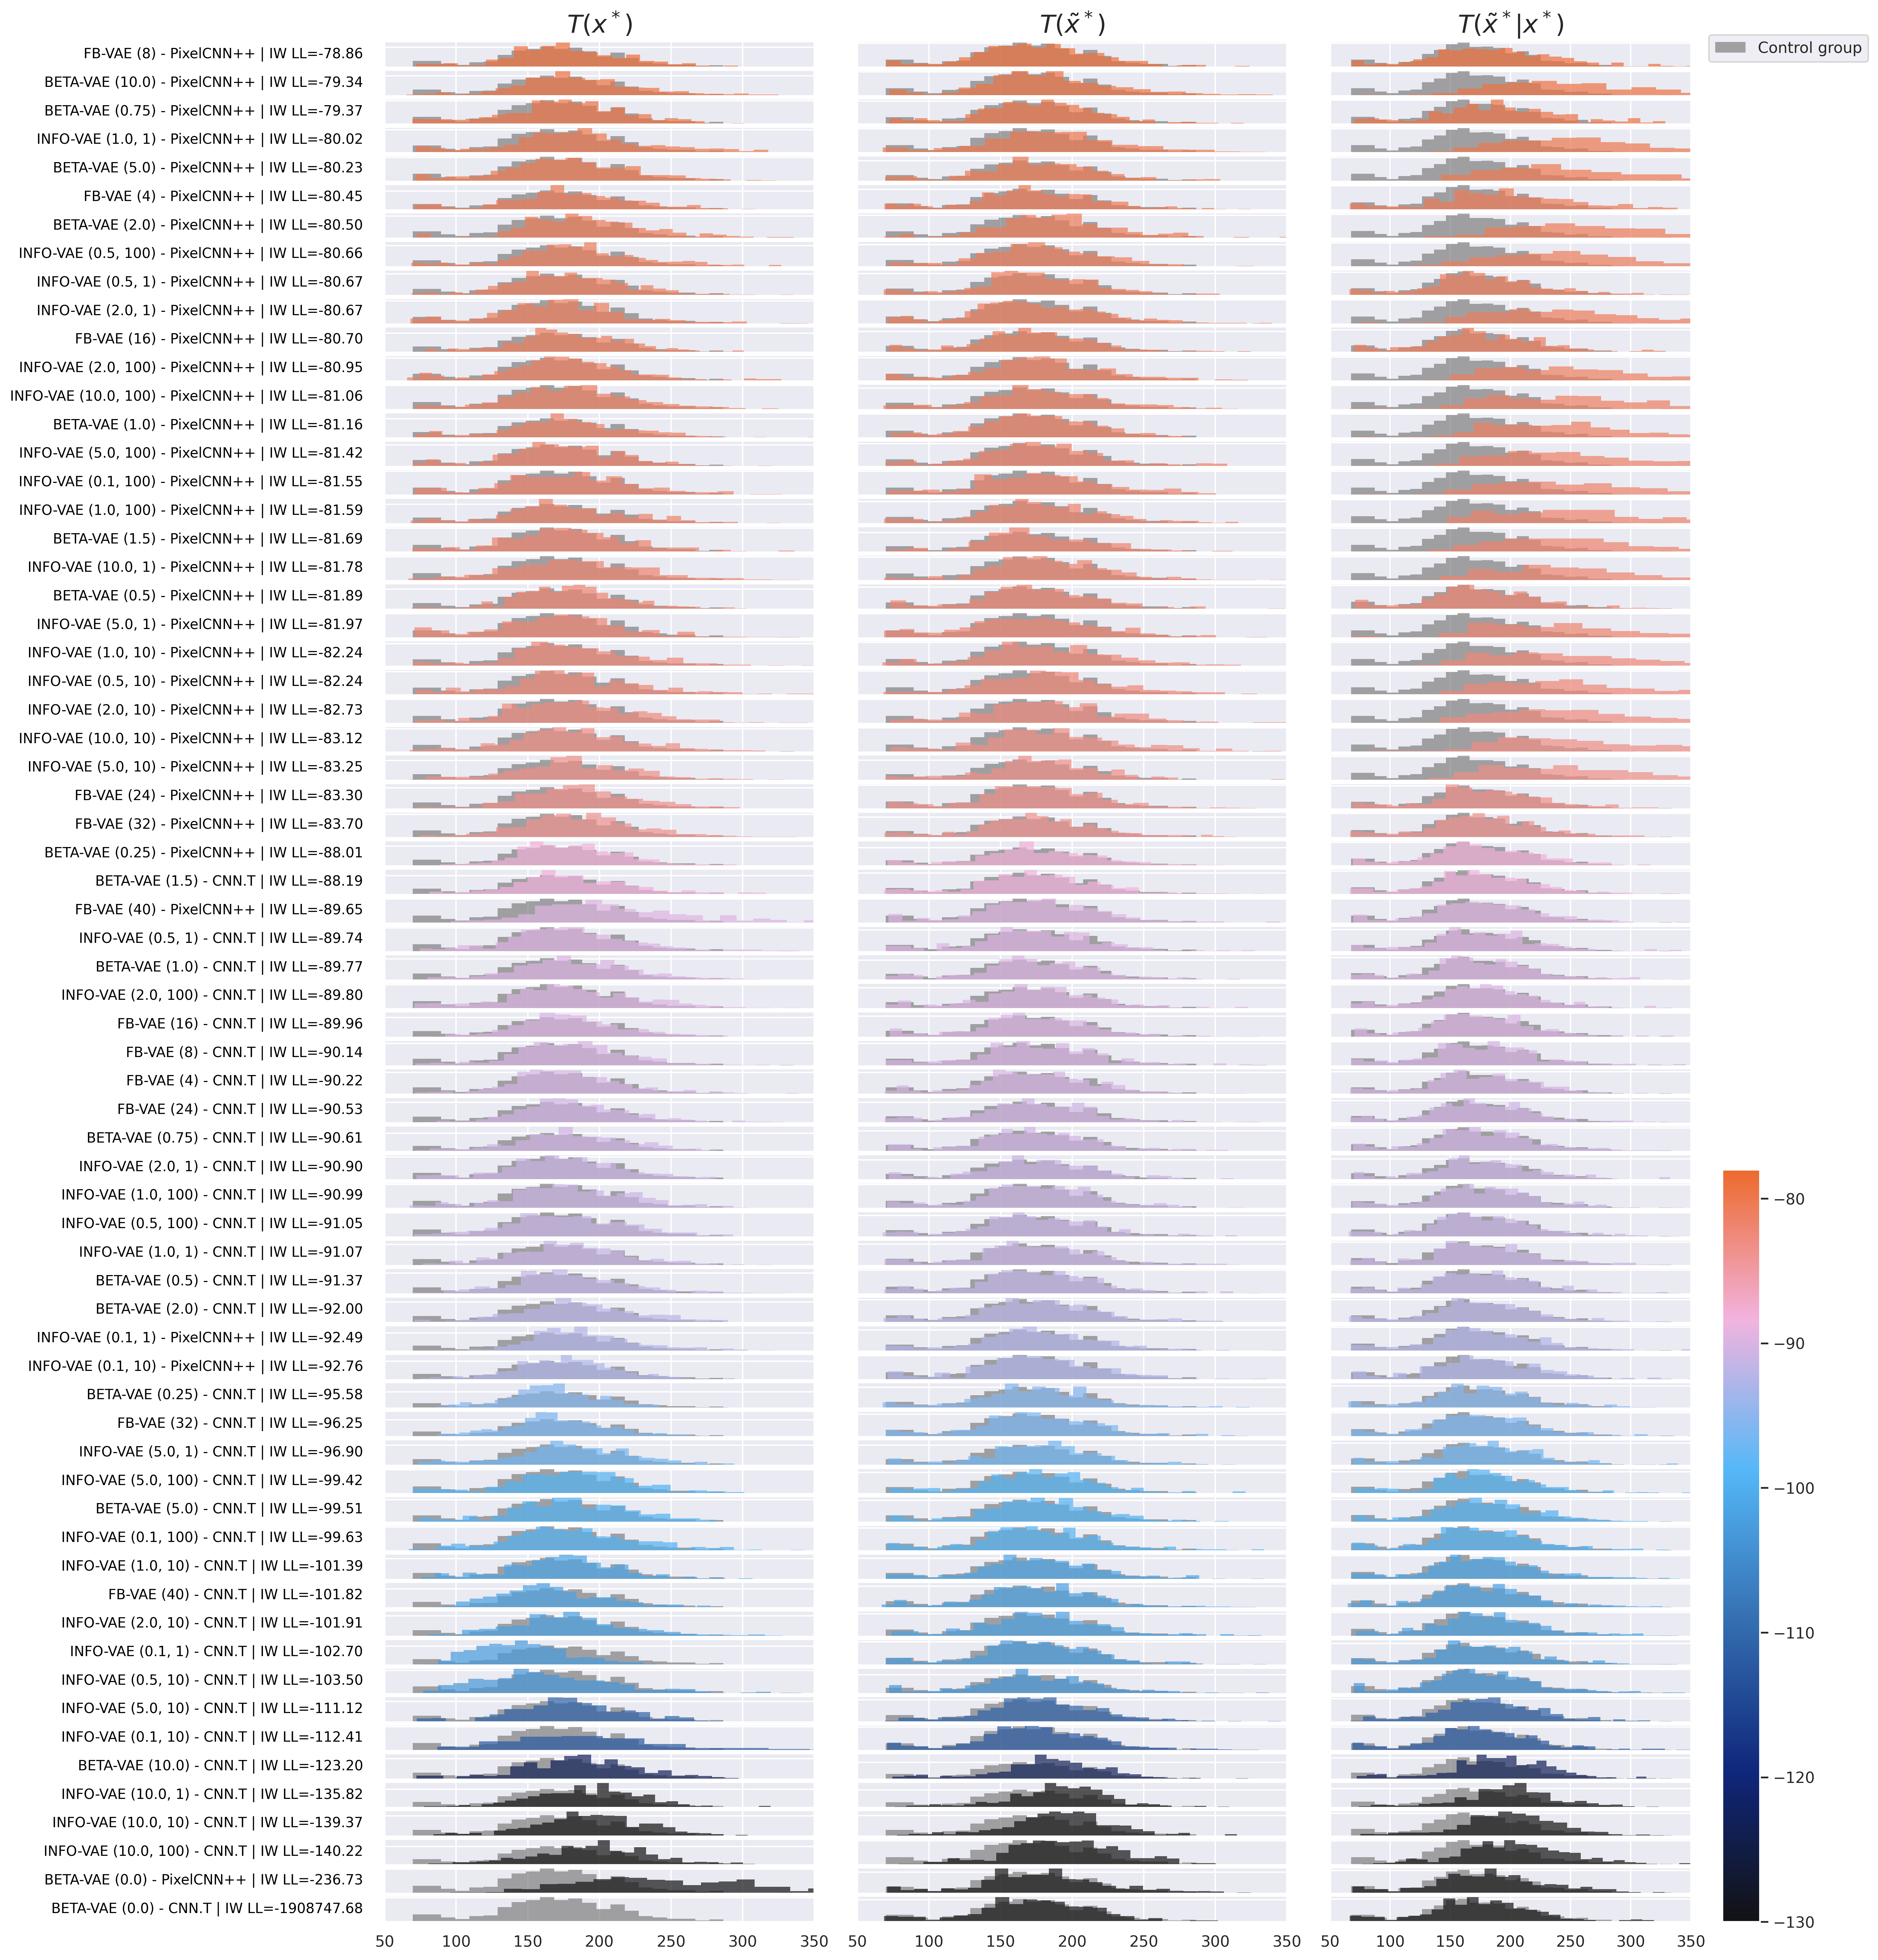
\includegraphics[width=\textwidth]{images/surprisal_dists/mnist_surprisal_dist.png}
    \caption{The three statistics $T(x^*)$, $T(\tilde x^*)$ and $T(\tilde x^*|x^*)$ based on the log posterior predictive density of the MNIST digit identity latent structure model of the experiments plotted against the respective control groups. The rows are ordered and coloured by an importance weighted estimate of the log likelihood (IW LL) of the VAEs on held-out data.}
    \label{fig:mnist_surprisal_dist}
\end{figure*}

% PTB sequence length surprisal distributions
\begin{figure*}[!htb]
    \centering
    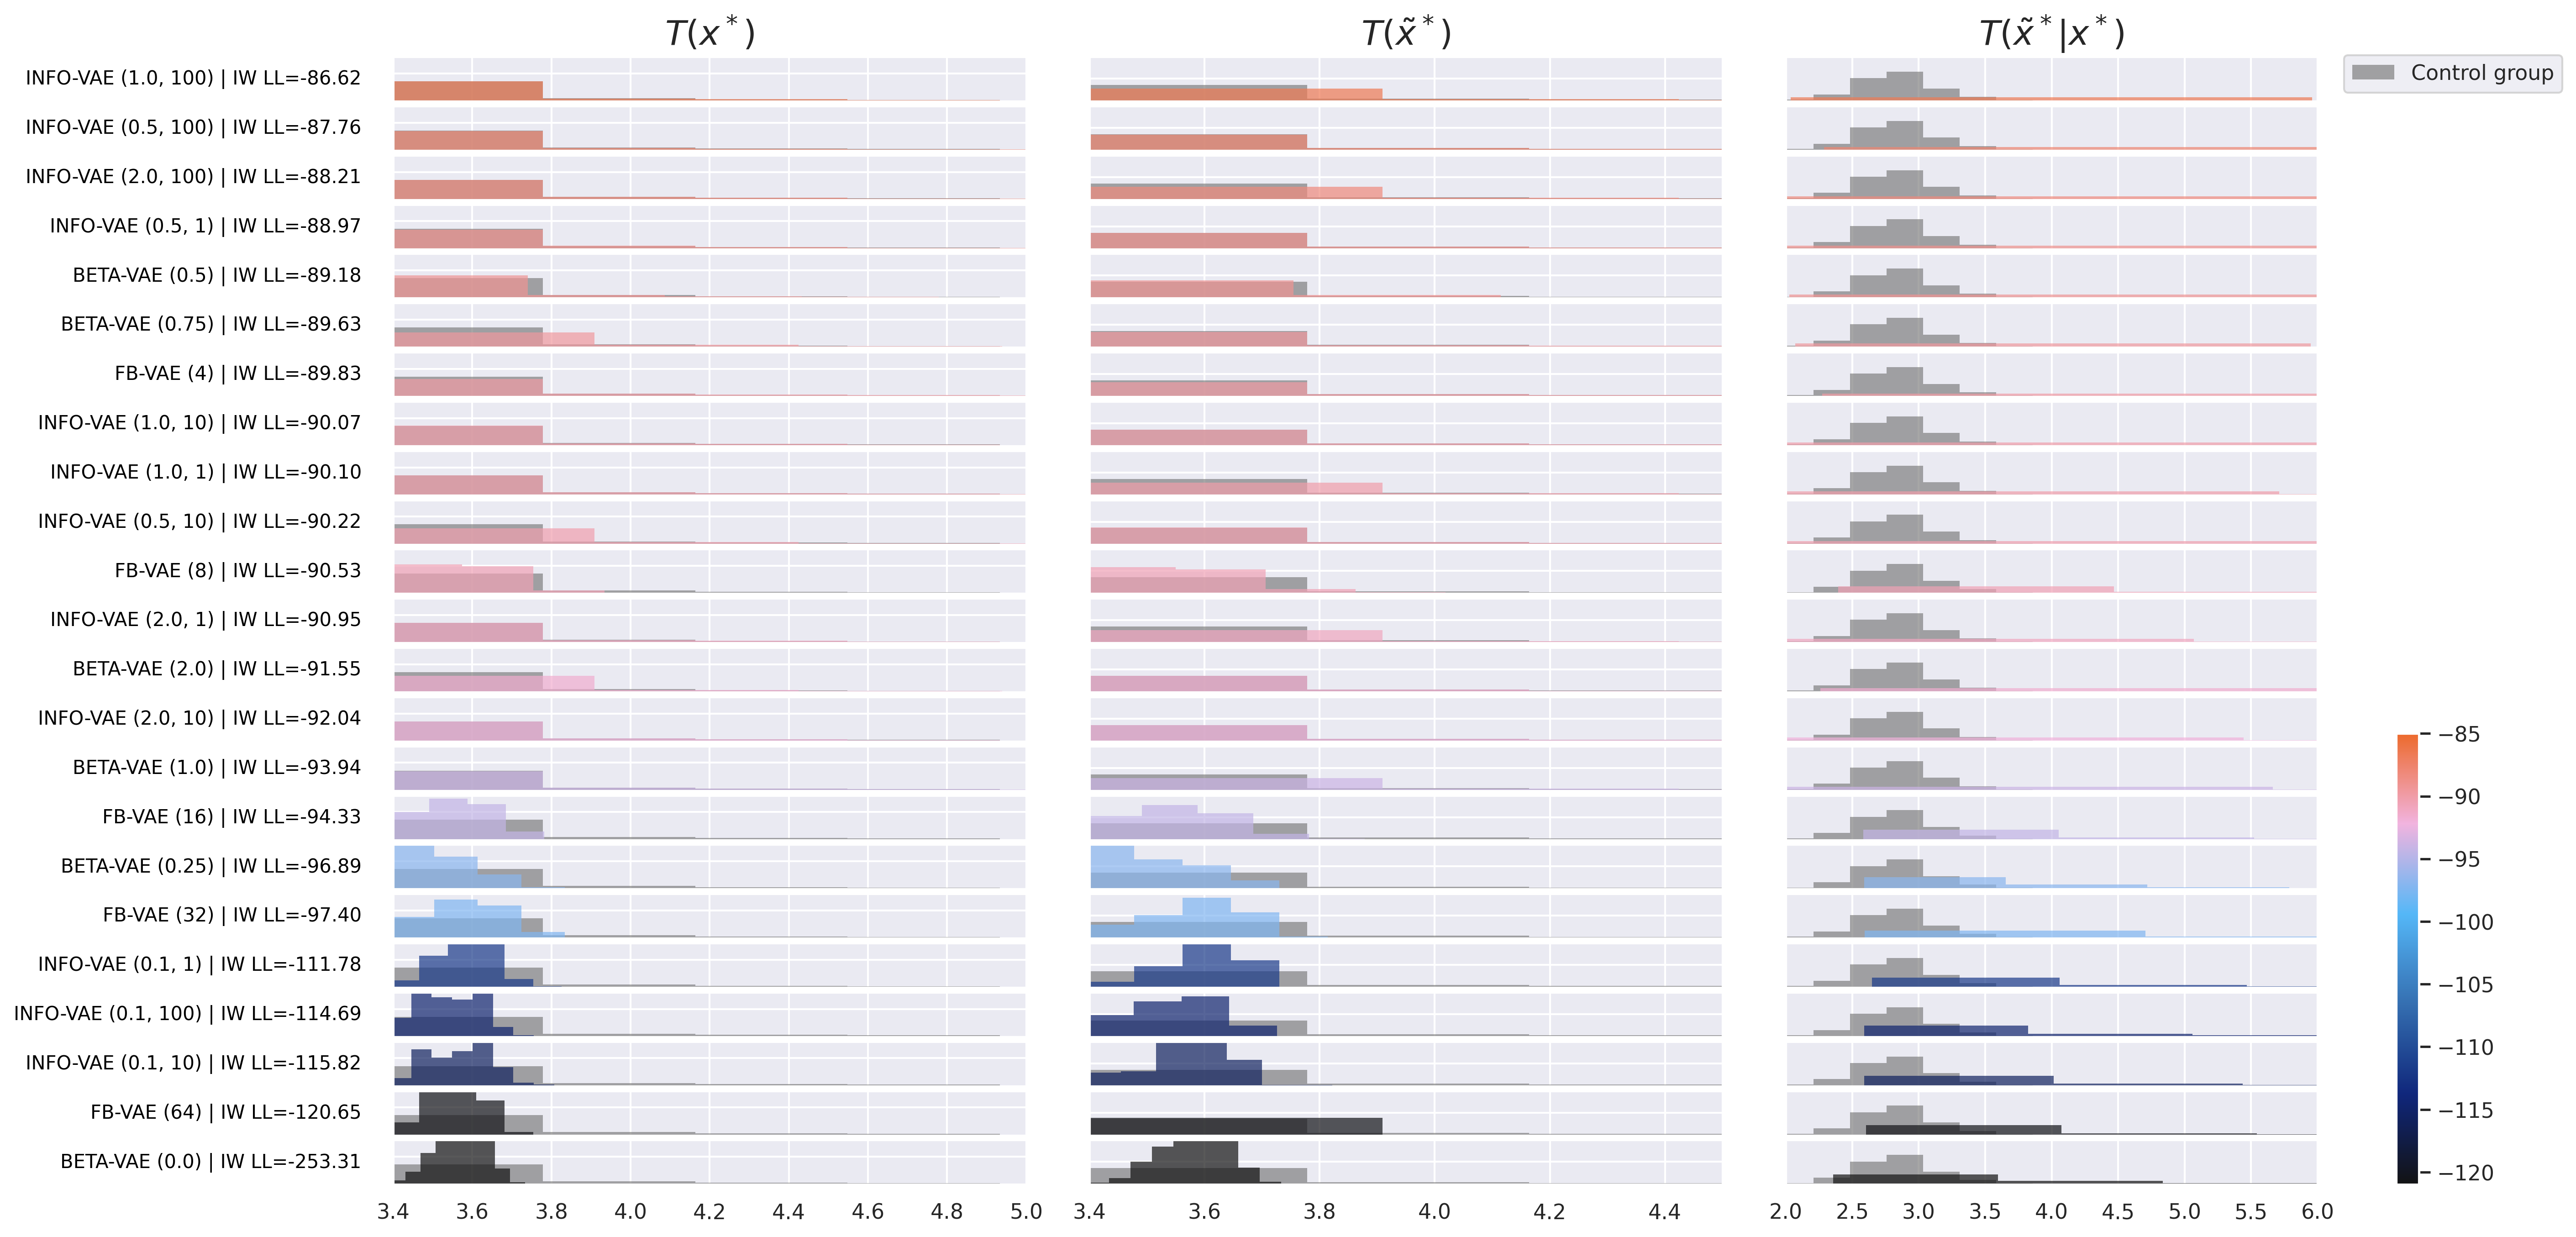
\includegraphics[width=\textwidth]{images/surprisal_dists/ptb_seq_len_surprisal_dist.png}
    \caption{The three statistics $T(x^*)$, $T(\tilde x^*)$ and $T(\tilde x^*|x^*)$ based on the log posterior predictive density of the PTB sequence length latent structure model of the experiments plotted against the respective control groups. The rows are ordered and coloured by an importance weighted estimate of the log likelihood (IW LL) of the VAEs on held-out data.}
    \label{fig:ptb_seq_len_surprisal_dist}
\end{figure*}

%PTB LDA surprisal distributions
\begin{figure*}[!htb]
    \centering
    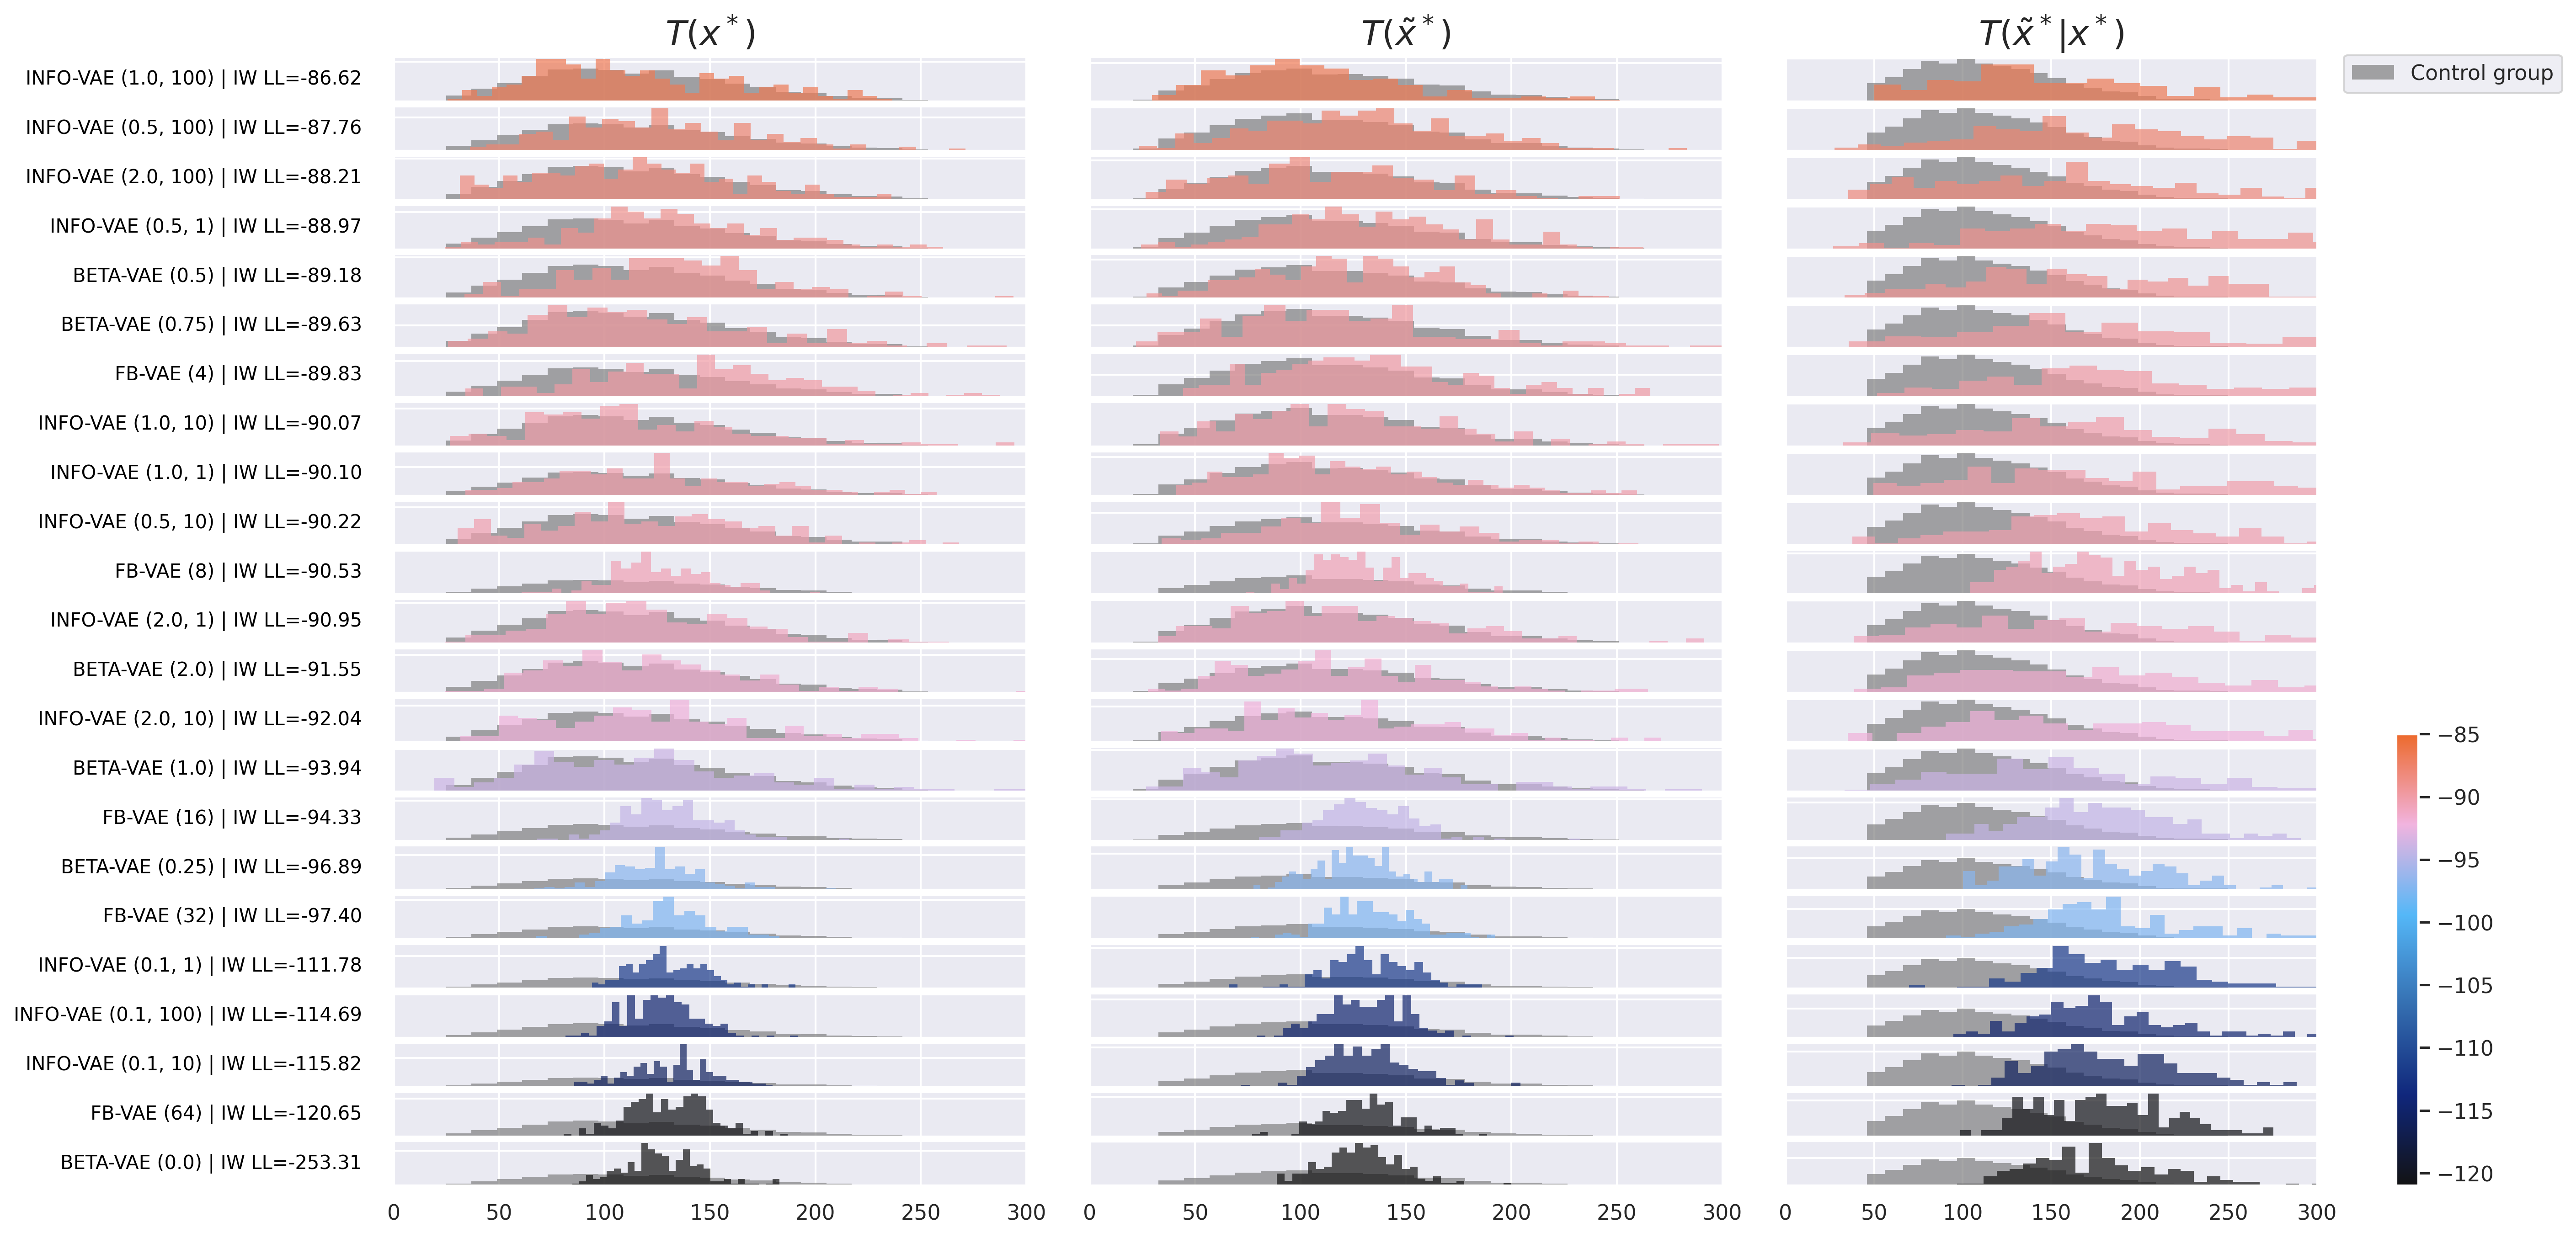
\includegraphics[width=\textwidth]{images/surprisal_dists/ptb_lda_topics_surprisal_dist.png}
    \caption{The three statistics $T(x^*)$, $T(\tilde x^*)$ and $T(\tilde x^*|x^*)$ based on the log posterior predictive density of the PTB topic latent structure model of the experiments plotted against the respective control groups. The rows are ordered and coloured by an importance weighted estimate of the log likelihood (IW LL) of the VAEs on held-out data.}
    \label{fig:ptb_lda_topics_surprisal_dist}
\end{figure*}

\section{Intrinsic evaluation results}\label{app:intrinsic-evaluation}

The full results as visualised in Figure \ref{fig:intrinsic-evaluation-plot} are listed in Tables \ref{tab:bmnist_full_results} and \ref{tab:ptb_full_results} for the binarised MNIST and PTB experiments respectively.

% Full intrinsic evaluation table BMNIST
\begin{table*}[!htb]
    \centering
    \scriptsize
    \begin{tabular}{llllll|rrrrr}
    \toprule
    Decoder & Objective & $\lambda_{\text{FB}}$ &  $\beta$ & $\lambda_{\text{MMD}}$ & $\lambda_{\text{rate}}$ &    IW LL &     ELBO &    Rate &  Distortion &        MMD \\
\midrule
      CNN.T &  BETA-VAE &         - &  0.00 &     - &      - & -1908747.684 & -1910785.802 & 1910706.699 &      79.108 &   0.265494 \\
 PixelCNN++ &  BETA-VAE &         - &  0.00 &     - &      - &     -236.732 &     -235.079 &     174.957 &      60.122 &   0.530988 \\
      CNN.T &  INFO-VAE &         - &      - &   100 & 10.0 &     -140.217 &     -157.334 &       3.218 &     154.116 &   0.000446 \\
      CNN.T &  INFO-VAE &         - &      - &    10 & 10.0 &     -139.367 &     -157.106 &       3.275 &     153.831 &   0.000721 \\
      CNN.T &  INFO-VAE &         - &      - &     1 & 10.0 &     -135.821 &     -155.290 &       3.412 &     151.878 &   0.000594 \\
      CNN.T &  BETA-VAE &         - & 10.00 &     - &      - &     -123.197 &     -142.718 &       4.104 &     138.614 &   0.000462 \\
      CNN.T &  INFO-VAE &         - &      - &    10 &  0.1 &     -112.413 &     -115.687 &      36.708 &      78.979 &   0.055015 \\
      CNN.T &  INFO-VAE &         - &      - &    10 &  5.0 &     -111.122 &     -122.567 &       8.437 &     114.130 &   0.004309 \\
      CNN.T &  INFO-VAE &         - &      - &    10 &  0.5 &     -103.501 &     -106.251 &      24.296 &      81.955 &   0.042997 \\
      CNN.T &  INFO-VAE &         - &      - &     1 &  0.1 &     -102.699 &     -105.651 &      37.987 &      67.665 &   0.109114 \\
      CNN.T &  INFO-VAE &         - &      - &    10 &  2.0 &     -101.911 &     -107.297 &      14.748 &      92.550 &   0.009465 \\
      CNN.T &    FB-VAE &        40 &      - &     - &      - &     -101.823 &     -104.936 &      37.671 &      67.265 &   0.131946 \\
      CNN.T &  INFO-VAE &         - &      - &    10 &  1.0 &     -101.392 &     -103.785 &      19.484 &      84.300 &   0.016348 \\
      CNN.T &  INFO-VAE &         - &      - &   100 &  0.1 &      -99.630 &     -102.594 &      34.361 &      68.233 &   0.003865 \\
      CNN.T &  BETA-VAE &         - &  5.00 &     - &      - &      -99.506 &     -111.420 &       9.002 &     102.418 &   0.001213 \\
      CNN.T &  INFO-VAE &         - &      - &   100 &  5.0 &      -99.419 &     -111.431 &       9.074 &     102.356 &   0.001087 \\
      CNN.T &  INFO-VAE &         - &      - &     1 &  5.0 &      -96.905 &     -111.545 &       8.959 &     102.586 &   0.001620 \\
      CNN.T &    FB-VAE &        32 &      - &     - &      - &      -96.250 &      -99.154 &      30.607 &      68.547 &   0.054848 \\
      CNN.T &  BETA-VAE &         - &  0.25 &     - &      - &      -95.583 &      -98.752 &      30.788 &      67.964 &   0.054161 \\
 PixelCNN++ &  INFO-VAE &         - &      - &    10 &  0.1 &      -92.755 &      -96.713 &      35.803 &      60.910 &   0.021386 \\
 PixelCNN++ &  INFO-VAE &         - &      - &     1 &  0.1 &      -92.494 &      -96.655 &      46.089 &      50.566 &   0.063386 \\
      CNN.T &  BETA-VAE &         - &  2.00 &     - &      - &      -92.004 &      -95.649 &      15.915 &      79.735 &   0.006296 \\
      CNN.T &  BETA-VAE &         - &  0.50 &     - &      - &      -91.366 &      -95.277 &      25.682 &      69.595 &   0.021536 \\
      CNN.T &  INFO-VAE &         - &      - &     1 &  1.0 &      -91.075 &      -93.643 &      20.741 &      72.901 &   0.010445 \\
      CNN.T &  INFO-VAE &         - &      - &   100 &  0.5 &      -91.047 &      -94.688 &      25.119 &      69.568 &   0.002931 \\
      CNN.T &  INFO-VAE &         - &      - &   100 &  1.0 &      -90.987 &      -93.405 &      20.492 &      72.913 &   0.002752 \\
      CNN.T &  INFO-VAE &         - &      - &     1 &  2.0 &      -90.903 &      -95.517 &      15.738 &      79.779 &   0.004205 \\
      CNN.T &  BETA-VAE &         - &  0.75 &     - &      - &      -90.609 &      -93.535 &      22.650 &      70.885 &   0.014209 \\
      CNN.T &    FB-VAE &        24 &      - &     - &      - &      -90.534 &      -94.576 &      24.228 &      70.348 &   0.019529 \\
      CNN.T &    FB-VAE &         4 &      - &     - &      - &      -90.221 &      -93.075 &      20.691 &      72.385 &   0.009502 \\
      CNN.T &    FB-VAE &         8 &      - &     - &      - &      -90.140 &      -93.111 &      20.838 &      72.272 &   0.012566 \\
      CNN.T &    FB-VAE &        16 &      - &     - &      - &      -89.955 &      -93.511 &      21.312 &      72.199 &   0.012732 \\
      CNN.T &  INFO-VAE &         - &      - &   100 &  2.0 &      -89.805 &      -95.291 &      15.892 &      79.399 &   0.002115 \\
      CNN.T &  BETA-VAE &         - &  1.00 &     - &      - &      -89.767 &      -93.170 &      20.516 &      72.654 &   0.009939 \\
      CNN.T &  INFO-VAE &         - &      - &     1 &  0.5 &      -89.740 &      -94.728 &      25.616 &      69.112 &   0.020474 \\
 PixelCNN++ &    FB-VAE &        40 &      - &     - &      - &      -89.652 &      -91.937 &      38.192 &      53.746 &   0.088447 \\
      CNN.T &  BETA-VAE &         - &  1.50 &     - &      - &      -88.192 &      -93.665 &      18.052 &      75.612 &   0.006233 \\
 PixelCNN++ &  BETA-VAE &         - &  0.25 &     - &      - &      -88.009 &      -90.369 &      38.595 &      51.773 &   0.026900 \\
 PixelCNN++ &    FB-VAE &        32 &      - &     - &      - &      -83.701 &      -86.769 &      31.107 &      55.661 &   0.024090 \\
 PixelCNN++ &    FB-VAE &        24 &      - &     - &      - &      -83.304 &      -84.196 &      23.840 &      60.356 &   0.008685 \\
 PixelCNN++ &  INFO-VAE &         - &      - &    10 &  5.0 &      -83.249 &      -82.019 &       0.000 &      82.018 &  -0.000051 \\
 PixelCNN++ &  INFO-VAE &         - &      - &    10 & 10.0 &      -83.124 &      -82.152 &       0.000 &      82.152 &   0.000044 \\
 PixelCNN++ &  INFO-VAE &         - &      - &    10 &  2.0 &      -82.733 &      -81.971 &       0.000 &      81.970 &  -0.000009 \\
 PixelCNN++ &  INFO-VAE &         - &      - &    10 &  0.5 &      -82.244 &      -82.234 &       0.002 &      82.232 &   0.000076 \\
 PixelCNN++ &  INFO-VAE &         - &      - &    10 &  1.0 &      -82.243 &      -82.169 &       0.001 &      82.169 &  -0.000157 \\
 PixelCNN++ &  INFO-VAE &         - &      - &     1 &  5.0 &      -81.965 &      -80.716 &       0.000 &      80.716 &   0.000060 \\
 PixelCNN++ &  BETA-VAE &         - &  0.50 &     - &      - &      -81.886 &      -84.875 &      26.952 &      57.923 &   0.006013 \\
 PixelCNN++ &  INFO-VAE &         - &      - &     1 & 10.0 &      -81.783 &      -82.144 &       0.000 &      82.144 &  -0.000015 \\
 PixelCNN++ &  BETA-VAE &         - &  1.50 &     - &      - &      -81.690 &      -80.745 &       0.000 &      80.745 &  -0.000073 \\
 PixelCNN++ &  INFO-VAE &         - &      - &   100 &  1.0 &      -81.587 &      -80.926 &       0.003 &      80.923 &  -0.000021 \\
 PixelCNN++ &  INFO-VAE &         - &      - &   100 &  0.1 &      -81.552 &      -80.771 &       0.004 &      80.767 &   0.000193 \\
 PixelCNN++ &  INFO-VAE &         - &      - &   100 &  5.0 &      -81.419 &      -80.846 &       0.003 &      80.843 &   0.000667 \\
 PixelCNN++ &  BETA-VAE &         - &  1.00 &     - &      - &      -81.165 &      -80.664 &       0.001 &      80.663 &   0.000035 \\
 PixelCNN++ &  INFO-VAE &         - &      - &   100 & 10.0 &      -81.058 &      -81.975 &       0.001 &      81.974 &  -0.000118 \\
 PixelCNN++ &  INFO-VAE &         - &      - &   100 &  2.0 &      -80.952 &      -80.756 &       0.011 &      80.744 &   0.000926 \\
 PixelCNN++ &    FB-VAE &        16 &      - &     - &      - &      -80.698 &      -81.895 &      16.927 &      64.968 &   0.002087 \\
 PixelCNN++ &  INFO-VAE &         - &      - &     1 &  2.0 &      -80.670 &      -80.555 &       0.003 &      80.553 &   0.000333 \\
 PixelCNN++ &  INFO-VAE &         - &      - &     1 &  0.5 &      -80.669 &      -84.514 &      26.190 &      58.324 &   0.003956 \\
 PixelCNN++ &  INFO-VAE &         - &      - &   100 &  0.5 &      -80.658 &      -80.769 &       0.003 &      80.766 &   0.000000 \\
 PixelCNN++ &  BETA-VAE &         - &  2.00 &     - &      - &      -80.505 &      -80.817 &       0.000 &      80.817 &   0.000025 \\
 PixelCNN++ &    FB-VAE &         4 &      - &     - &      - &      -80.446 &      -80.548 &       5.755 &      74.794 &   0.000707 \\
 PixelCNN++ &  BETA-VAE &         - &  5.00 &     - &      - &      -80.228 &      -80.670 &       0.000 &      80.669 &   0.000144 \\
 PixelCNN++ &  INFO-VAE &         - &      - &     1 &  1.0 &      -80.023 &      -80.621 &       0.000 &      80.620 &   0.000174 \\
 PixelCNN++ &  BETA-VAE &         - &  0.75 &     - &      - &      -79.370 &      -80.819 &       8.785 &      72.034 &   0.000669 \\
 PixelCNN++ &  BETA-VAE &         - & 10.00 &     - &      - &      -79.335 &      -80.604 &       0.000 &      80.604 &  -0.000003 \\
 PixelCNN++ &    FB-VAE &         8 &      - &     - &      - &      -78.865 &      -80.663 &       9.761 &      70.902 &   0.001080 \\
\bottomrule
    \end{tabular}
    \caption{Full intrinsic evaluation results of experiments on Binarised MNIST dataset}
    \label{tab:bmnist_full_results}
\end{table*}

% Full intrinsic evaluation table PTB
\begin{table*}[!htb]
    \centering
    \scriptsize
    \begin{tabular}{llllll|rrrrr}
    \toprule
        Decoder & Objective & $\lambda_{\text{FB}}$ &  $\beta$ & $\lambda_{\text{MMD}}$ & $\lambda_{\text{rate}}$ &    IW LL &     ELBO &    Rate &  Distortion &        MMD \\
\midrule
 Distil roBERTa &  BETA-VAE &         - & 0.000 &     - &      - & -253.314 & -262.025 & 199.762 &      62.263 &   0.004164 \\
 Distil roBERTa &    FB-VAE &        64 &     - &     - &      - & -120.653 & -125.793 &  60.116 &      65.677 &   0.000889 \\
 Distil roBERTa &  INFO-VAE &         - &     - &    10 &  0.1 & -115.817 & -119.895 &  51.583 &      68.311 &   0.000932 \\
 Distil roBERTa &  INFO-VAE &         - &     - &   100 &  0.1 & -114.690 & -118.358 &  48.643 &      69.715 &   0.000672 \\
 Distil roBERTa &  INFO-VAE &         - &     - &     1 &  0.1 & -111.780 & -119.874 &  51.270 &      68.604 &   0.000934 \\
 Distil roBERTa &    FB-VAE &        32 &     - &     - &      - &  -97.405 & -103.309 &  30.311 &      72.998 &   0.000347 \\
 Distil roBERTa &  BETA-VAE &         - & 0.25 &     - &      - &  -96.893 & -101.637 &  26.318 &      75.319 &   0.000433 \\
 Distil roBERTa &    FB-VAE &        16 &     - &     - &      - &  -94.325 &  -95.389 &  15.632 &      79.757 &   0.000246 \\
 Distil roBERTa &  BETA-VAE &         - & 1.00 &     - &      - &  -93.939 &  -89.989 &   0.006 &      89.983 &   0.000011 \\
 Distil roBERTa &  INFO-VAE &         - &     - &    10 &  2.0 &  -92.038 &  -90.203 &   0.002 &      90.202 &  -0.000003 \\
 Distil roBERTa &  BETA-VAE &         - & 2.00 &     - &      - &  -91.553 &  -90.596 &   0.001 &      90.595 &   0.000004 \\
 Distil roBERTa &  INFO-VAE &         - &     - &     1 &  2.0 &  -90.949 &  -90.400 &   0.001 &      90.399 &   0.000003 \\
 Distil roBERTa &    FB-VAE &         8 &     - &     - &      - &  -90.527 &  -92.318 &   8.047 &      84.271 &   0.000134 \\
 Distil roBERTa &  INFO-VAE &         - &     - &    10 &  0.5 &  -90.219 &  -91.485 &   4.573 &      86.912 &   0.000085 \\
 Distil roBERTa &  INFO-VAE &         - &     - &     1 &  1.0 &  -90.100 &  -90.172 &   0.004 &      90.168 &   0.000018 \\
 Distil roBERTa &  INFO-VAE &         - &     - &    10 &  1.0 &  -90.073 &  -90.215 &   0.005 &      90.210 &  -0.000010 \\
 Distil roBERTa &    FB-VAE &         4 &     - &     - &      - &  -89.834 &  -91.519 &   3.829 &      87.690 &   0.000075 \\
 Distil roBERTa &  BETA-VAE &         - & 0.75 &     - &      - &  -89.629 &  -90.604 &   0.021 &      90.583 &   0.000017 \\
 Distil roBERTa &  BETA-VAE &         - & 0.50 &     - &      - &  -89.176 &  -91.301 &   4.669 &      86.632 &   0.000131 \\
 Distil roBERTa &  INFO-VAE &         - &     - &     1 &  0.5 &  -88.973 &  -91.410 &   4.468 &      86.943 &   0.000075 \\
 Distil roBERTa &  INFO-VAE &         - &     - &   100 &  2.0 &  -88.214 &  -90.436 &   0.002 &      90.434 &   0.000004 \\
 Distil roBERTa &  INFO-VAE &         - &     - &   100 &  0.5 &  -87.757 &  -91.146 &   3.669 &      87.477 &   0.000156 \\
 Distil roBERTa &  INFO-VAE &         - &     - &   100 &  1.0 &  -86.616 &  -90.574 &   0.004 &      90.570 &   0.000018 \\
\bottomrule
    \end{tabular}
    \caption{Full intrinsic evaluation results of experiments on Penn Treebank dataset}
    \label{tab:ptb_full_results}
\end{table*}


\section{Grouped mixed membership models}\label{app:dp-models}

To compare the statistic histograms across groups in a systematic way, we fit Dirichlet process mixed membership models to the scalar valued statistics with the group variable denoting the different experiments and control group. In total we fit 9 of these models for the three statistics across three latent structure models. We use a truncated Normal as family for the components and uniform priors for the location and scale parameters of these components. The number of components is 5 for both the statistics resulting from the sequence length model and topic model and 7 for the MNIST digit identity model.

Figures \ref{fig:surprisal_check_mnist_uncon_uncon} -- \ref{fig:surprisal_check_ptb_topics_con_con} depict posterior predictive samples for different groups under the analysis DP mixture models that are used to compare the statistics  $T(x^*)$,  $T(\tilde x^*)$ and $T(\tilde x^*|x^*)$ evaluated under the three latent structure models (the MNIST digit identity model, the Penn Treebank sequence length model and the Penn Treebank LDA topic model) for different groups. 

% SURPRISAL DP CHECKS MNIST 1
\begin{figure*}[!htb]
    \centering
    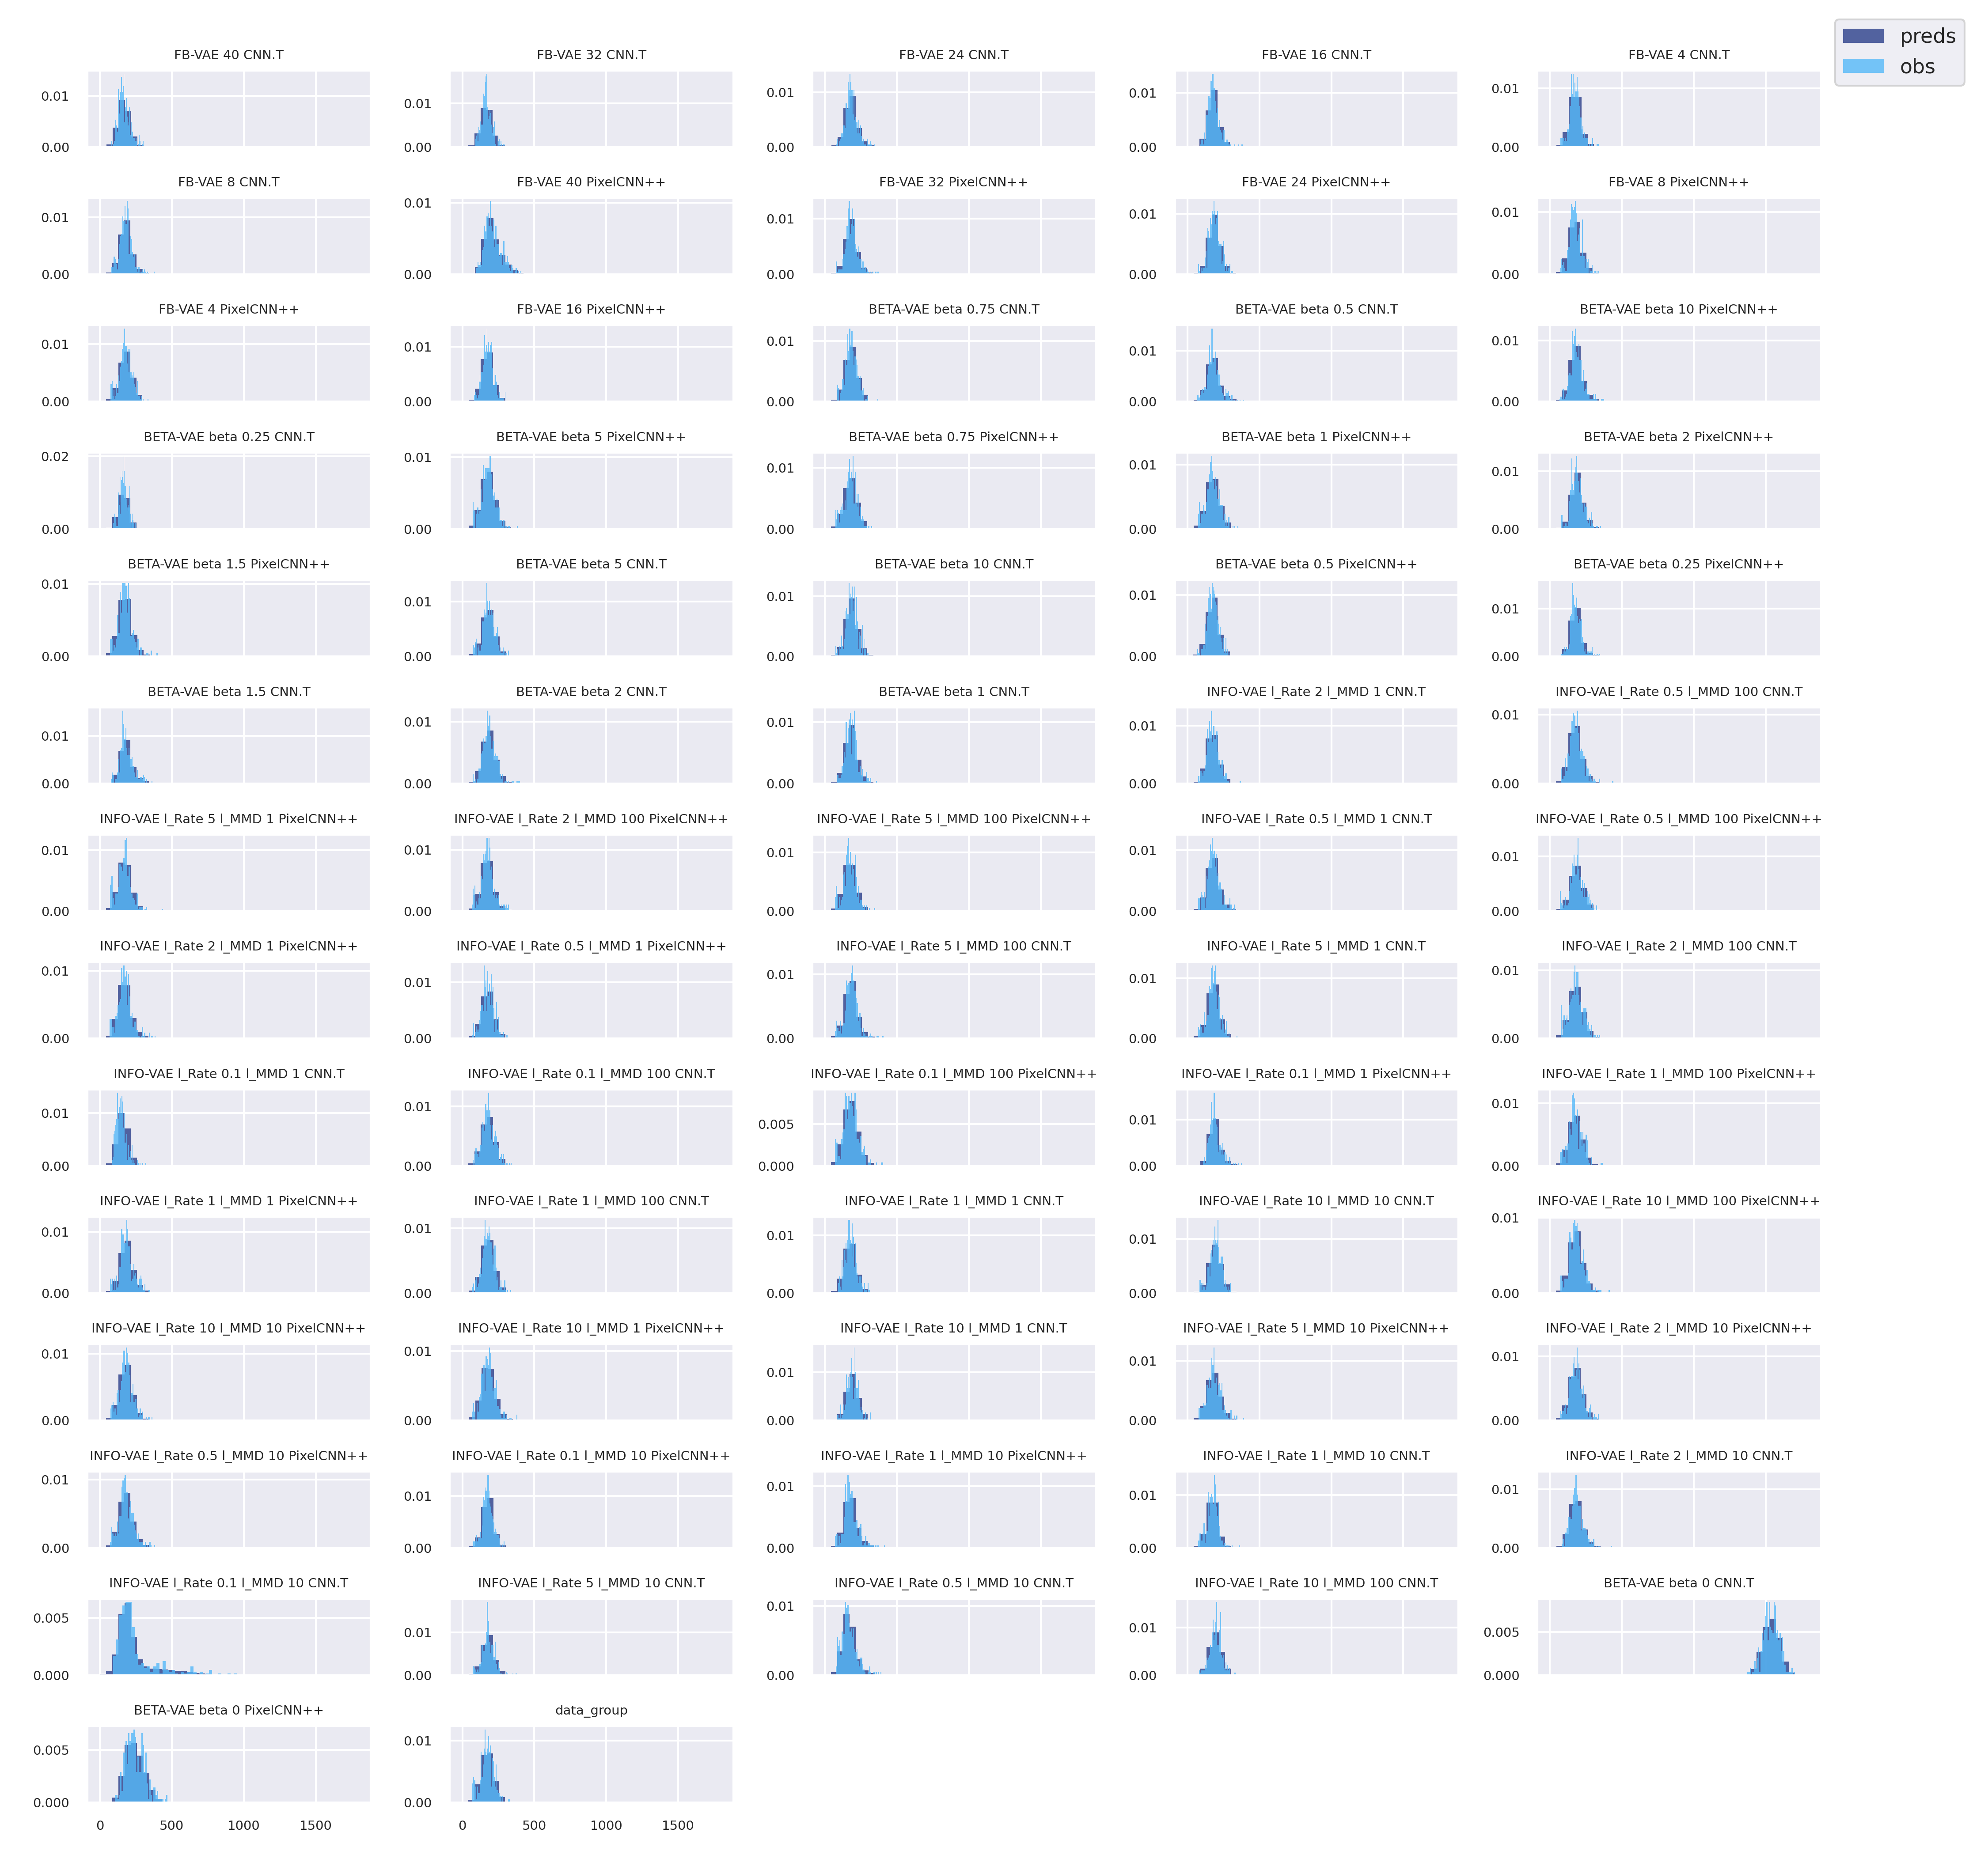
\includegraphics[width=\textwidth]{images/bda_checks/surprisal_dps/mnist_prediction_checks__unconditional_unconditional.png}
    \caption{Posterior predictive samples (preds) versus observations (obs) of the $T(x^*)$ statistic assessed under the MNIST digit identity latent structure model as modelled by the DP mixture model.}
    \label{fig:surprisal_check_mnist_uncon_uncon}
\end{figure*}

% SURPRISAL DP CHECKS MNIST 2
\begin{figure*}[!htb]
    \centering
    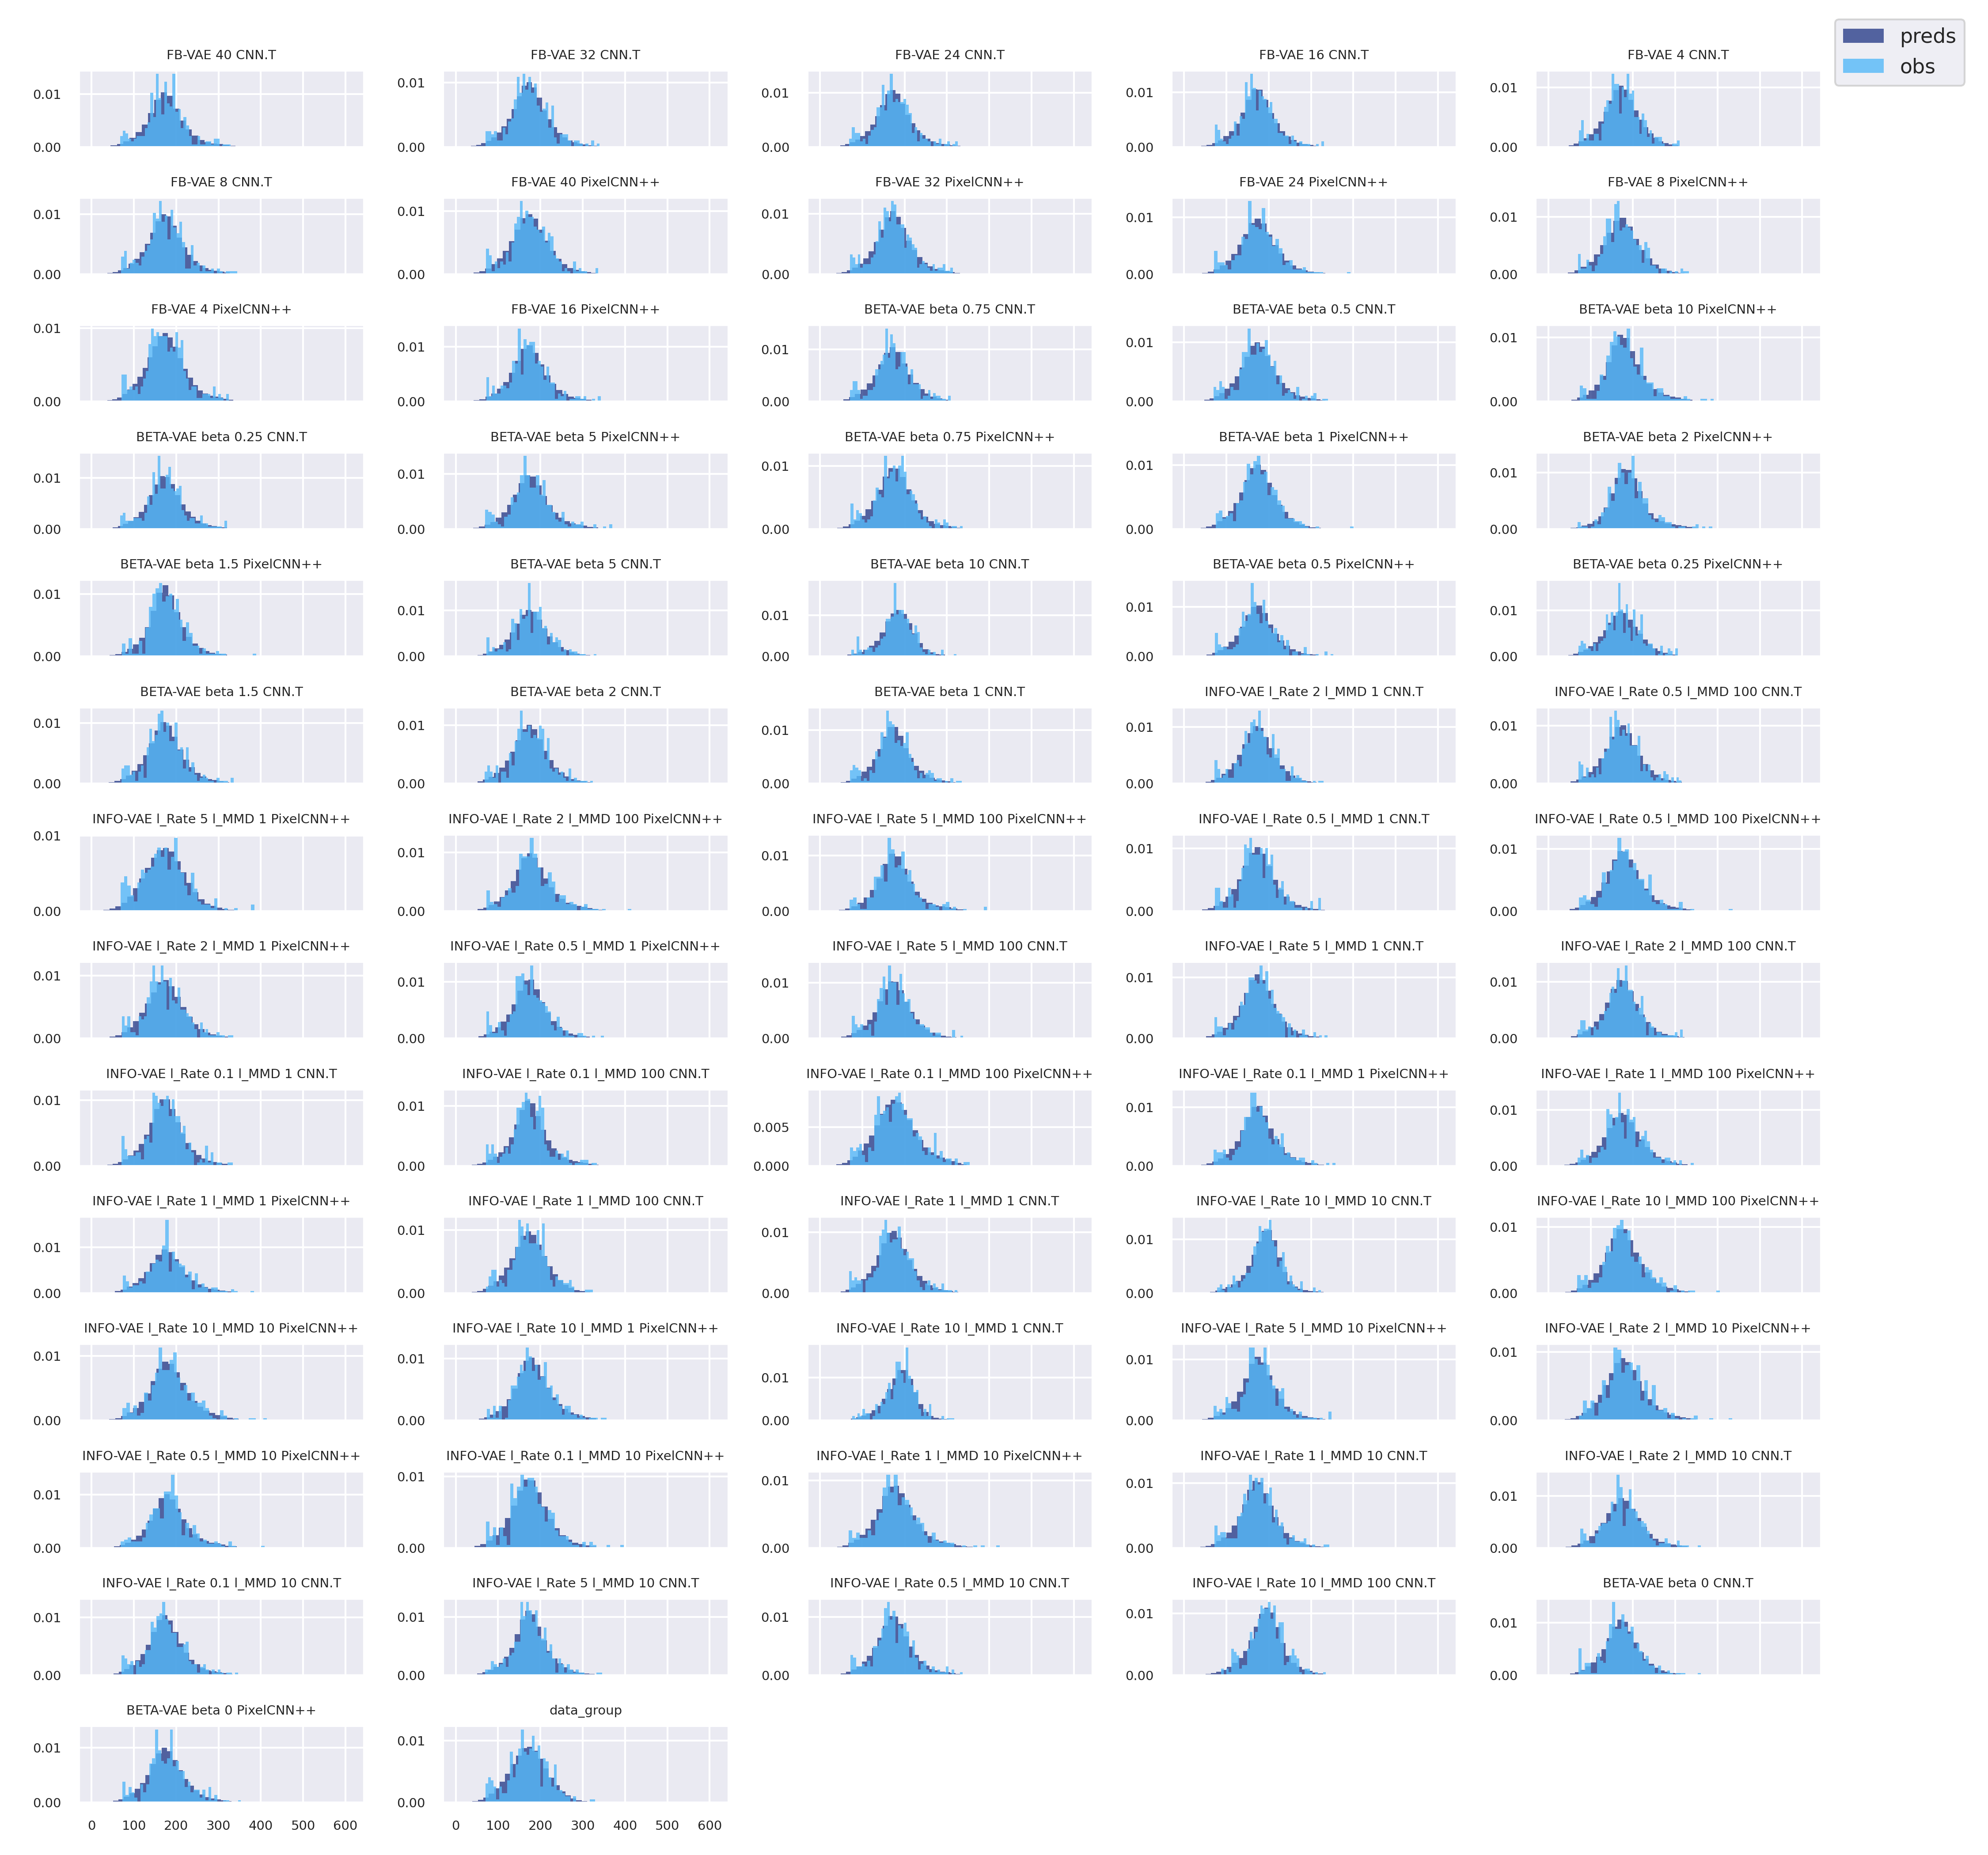
\includegraphics[width=\textwidth]{images/bda_checks/surprisal_dps/mnist_prediction_checks__unconditional_conditional.png}
    \caption{Posterior predictive samples (preds) versus observations (obs) of the $T(\tilde x^*)$ statistic assessed under the MNIST digit identity latent structure model as modelled by the DP mixture model.}
    \label{fig:surprisal_check_mnist_uncon_con}
\end{figure*}

% SURPRISAL DP CHECKS MNIST 3
\begin{figure*}[!htb]
    \centering
    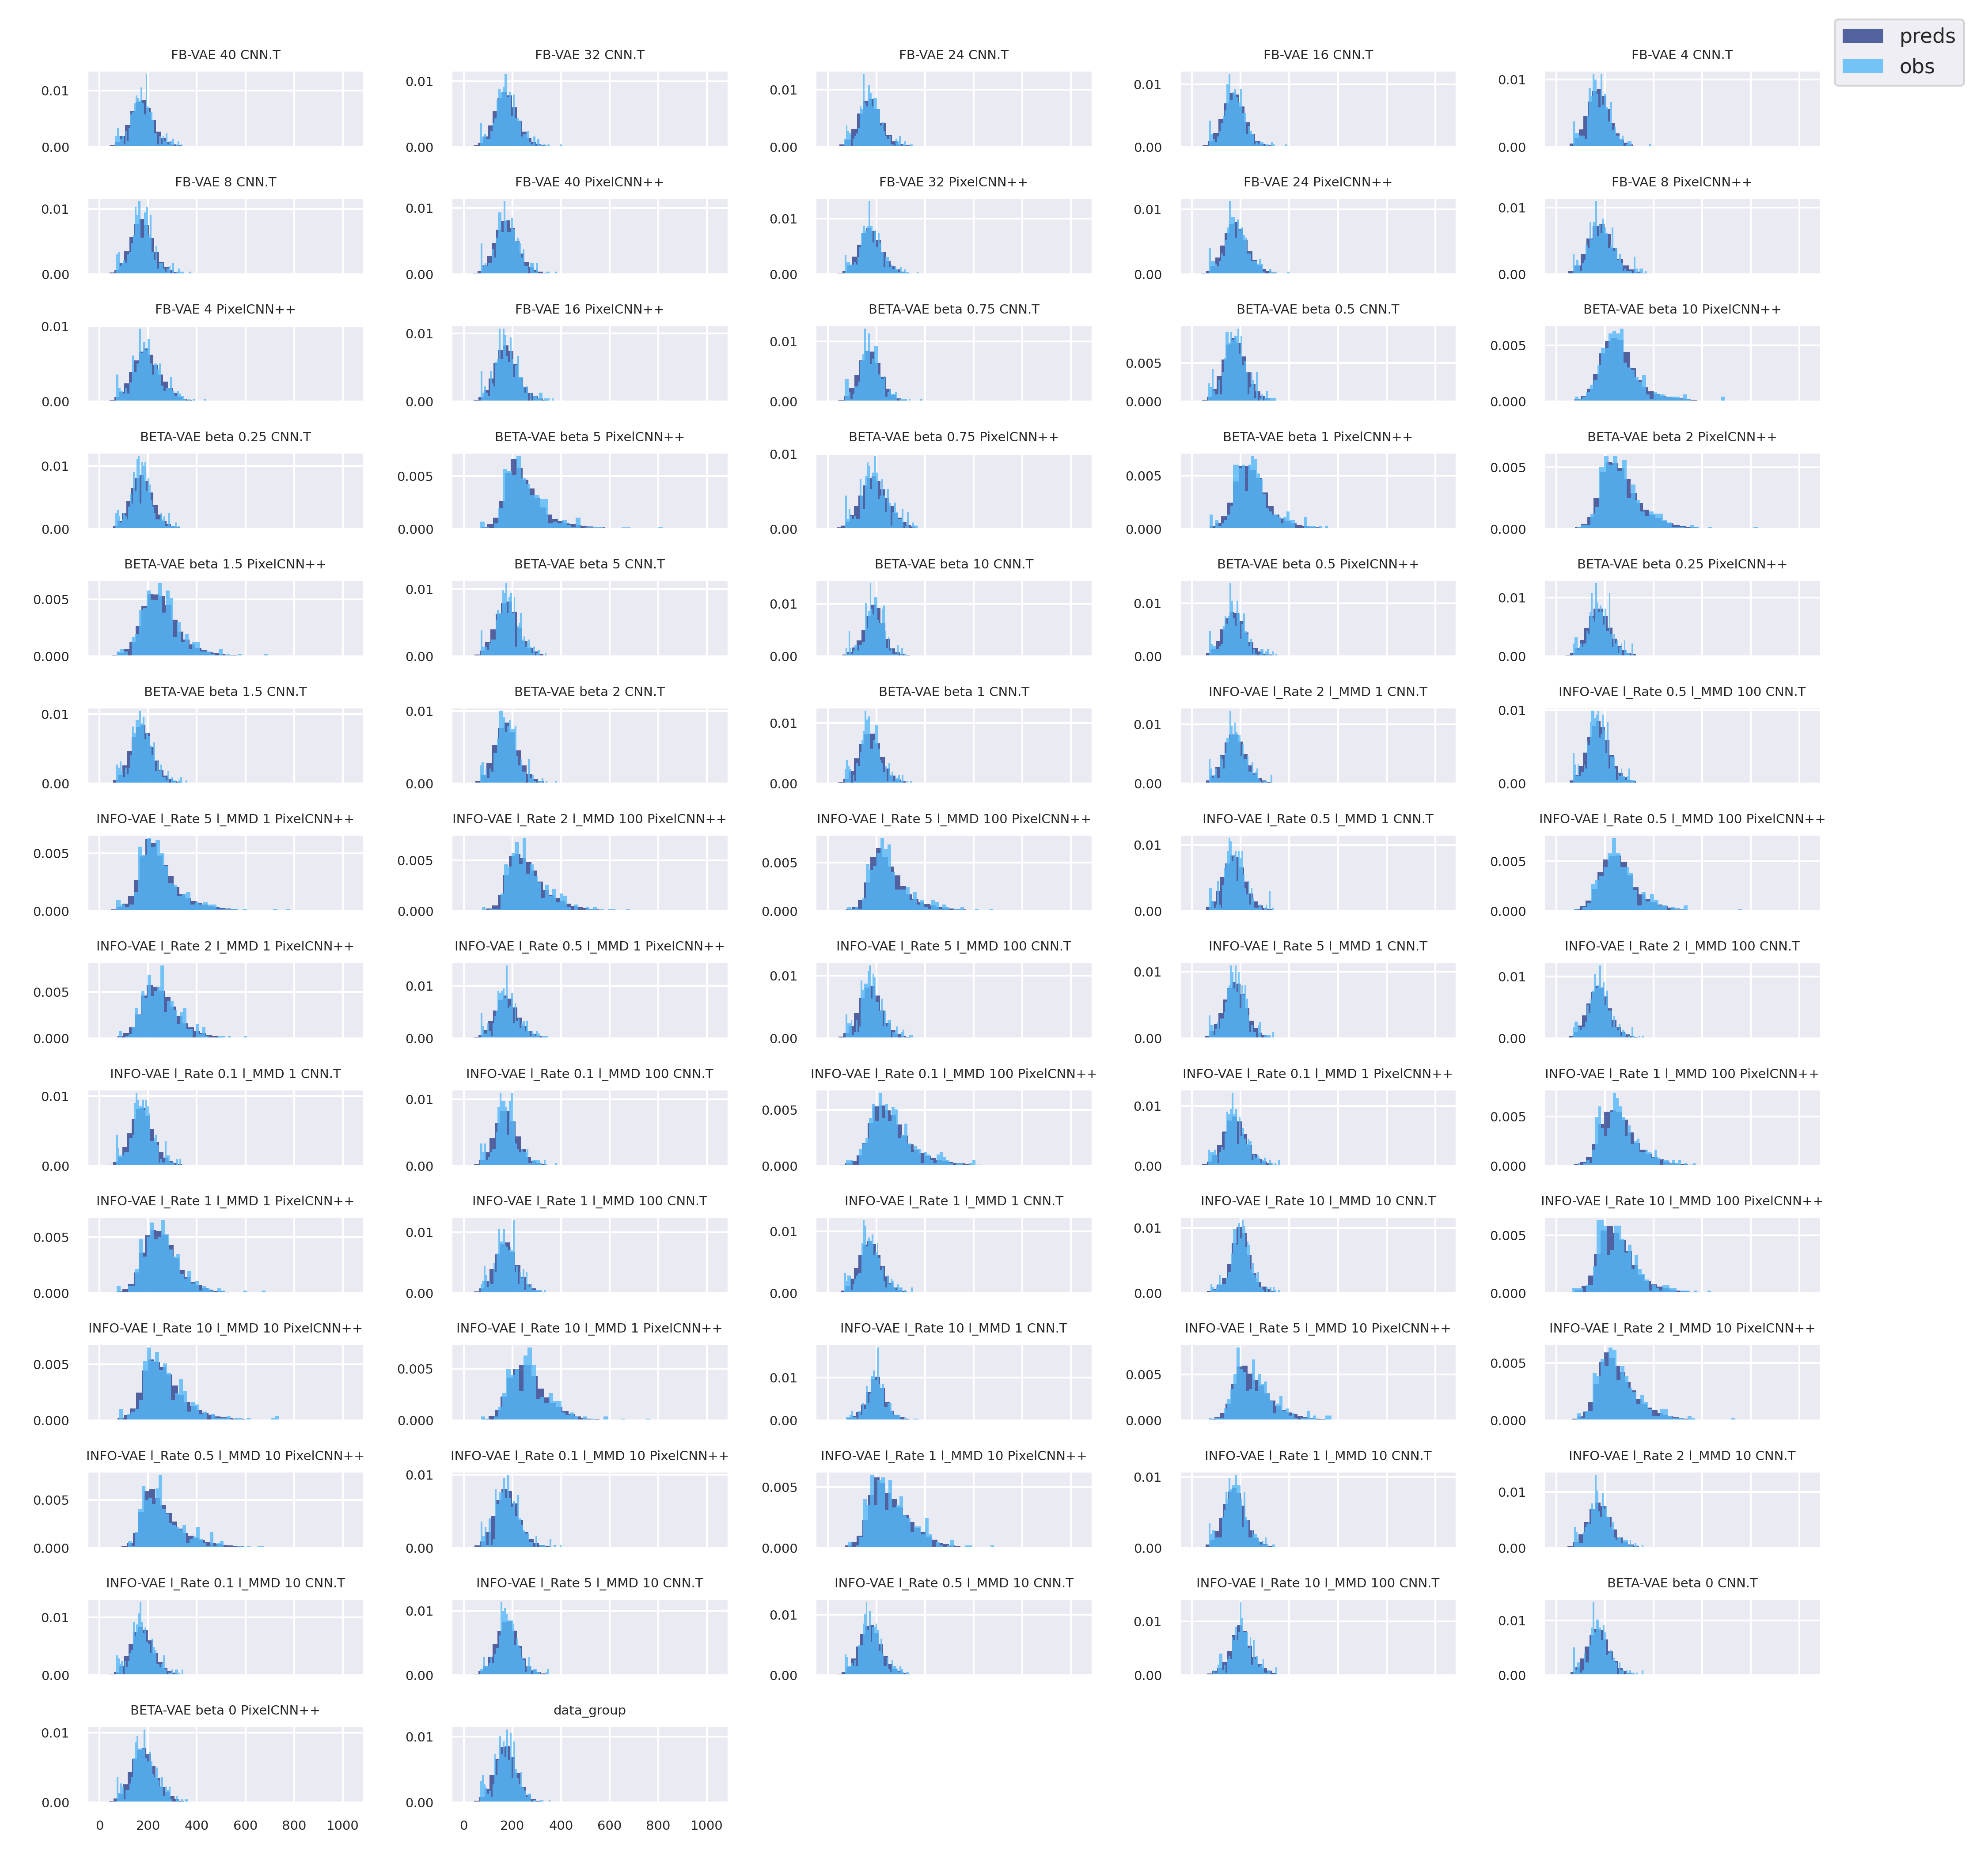
\includegraphics[width=\textwidth]{images/bda_checks/surprisal_dps/mnist_prediction_checks__conditional_conditional.png}
    \caption{Posterior predictive samples (preds) versus observations (obs) of the $T(\tilde x^* | x^*)$ statistic assessed under the MNIST digit identity latent structure model as modelled by the DP mixture model.}
    \label{fig:surprisal_check_mnist_con_con}
\end{figure*}

% SURPRISAL DP CHECKS PTB SEQ 1
\begin{figure*}[!htb]
    \centering
    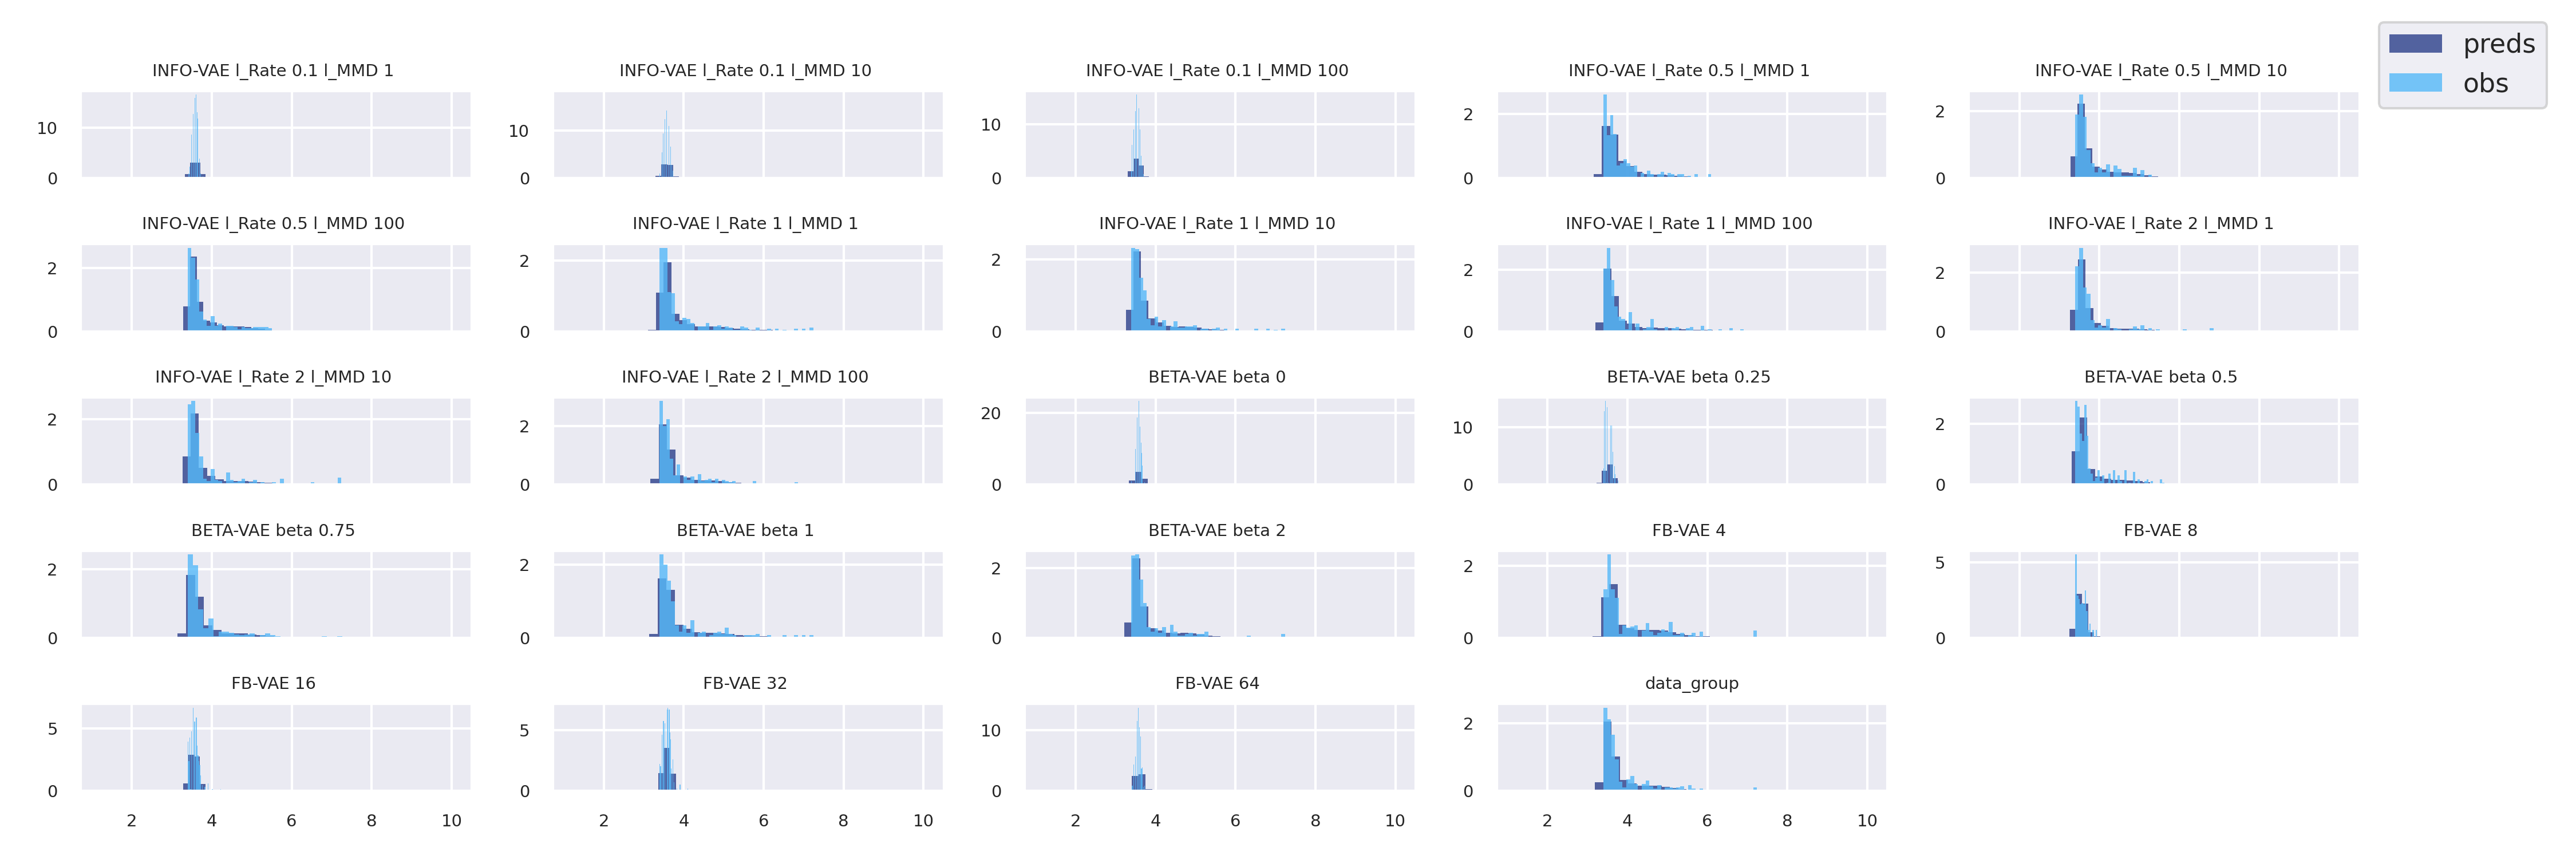
\includegraphics[width=\textwidth]{images/bda_checks/surprisal_dps/ptb_seq_len_prediction_checks__unconditional_unconditional.png}
    \caption{Posterior predictive samples (preds) versus observations (obs) of the $T(x^*)$ statistic assessed under the Penn Treebank sequence length latent structure model as modelled by the DP mixture model.}
    \label{fig:surprisal_check_ptb_seq_len_uncon_uncon}
\end{figure*}

% SURPRISAL DP CHECKS PTB SEQ 2
\begin{figure*}[!htb]
    \centering
    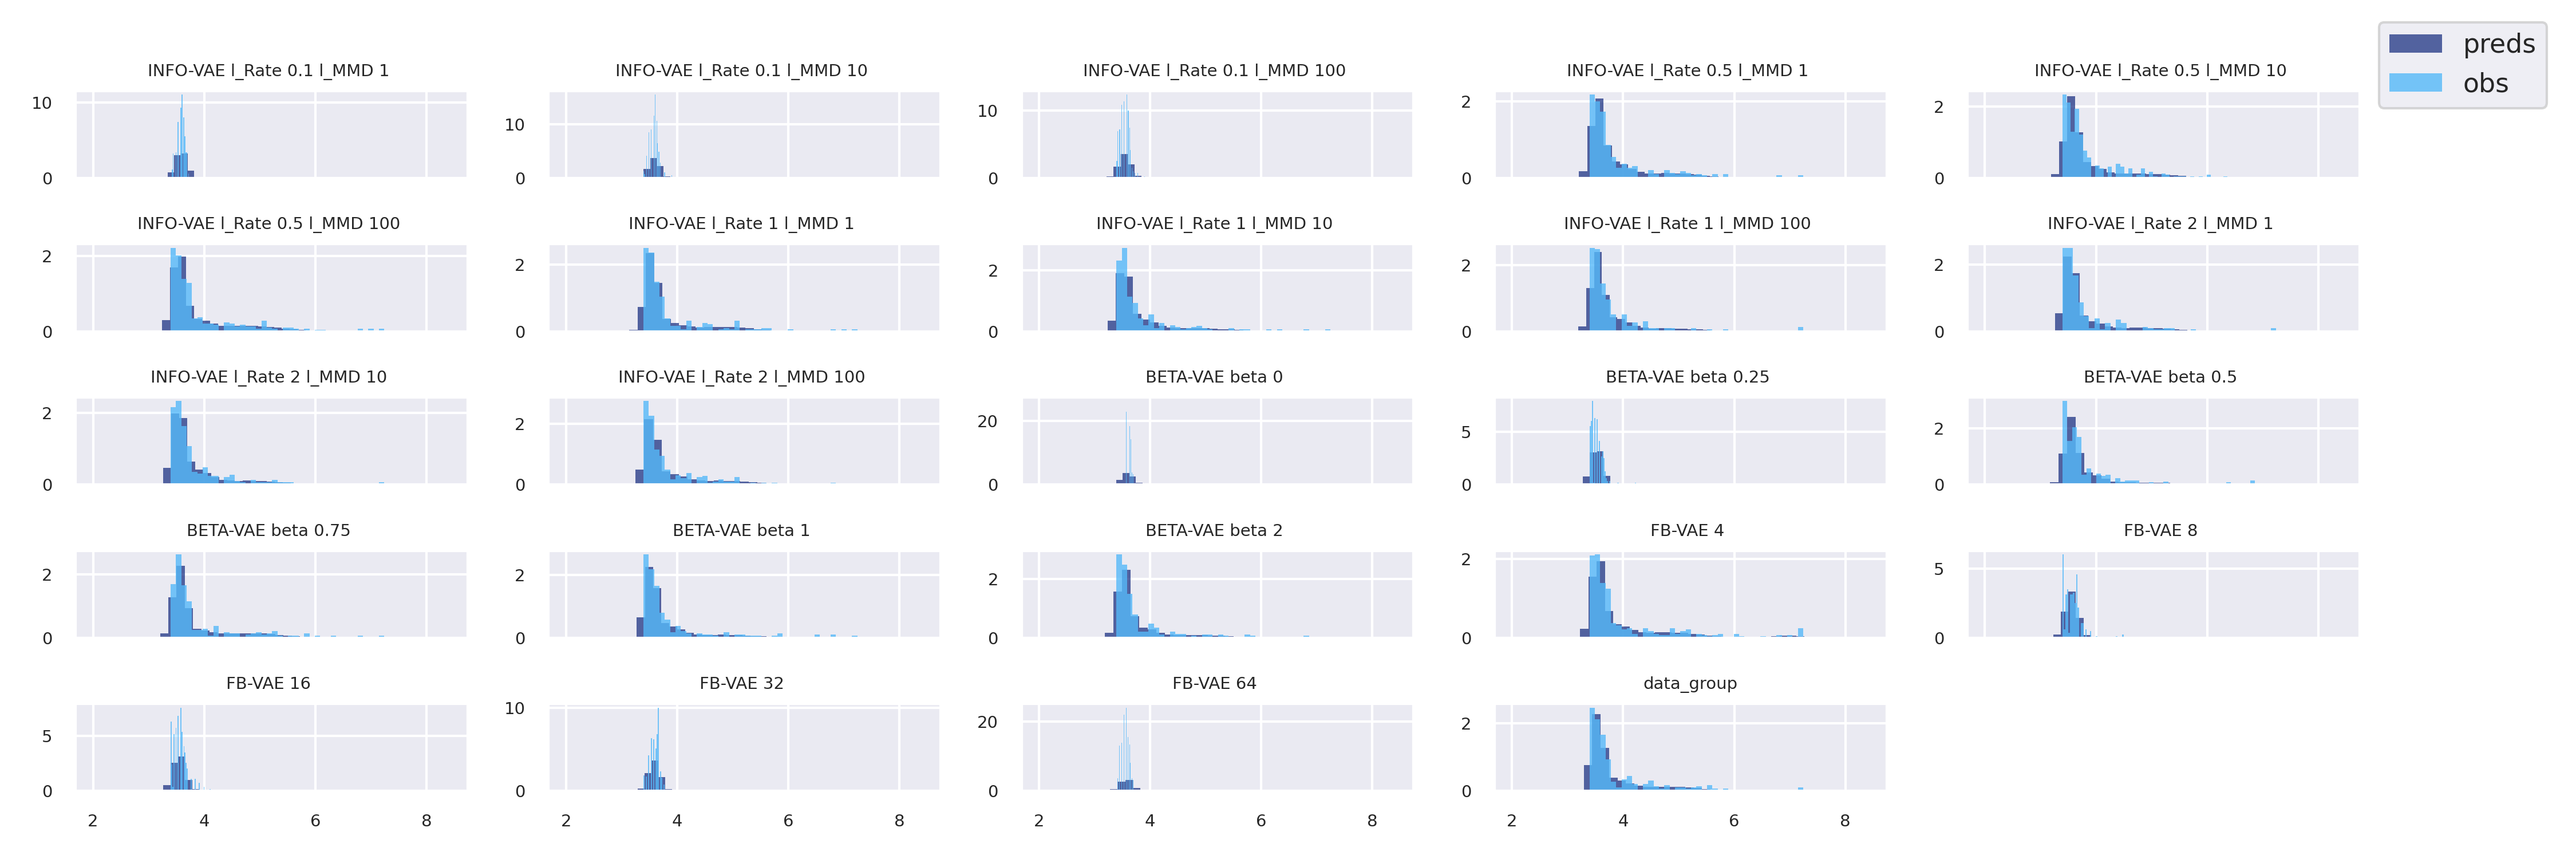
\includegraphics[width=\textwidth]{images/bda_checks/surprisal_dps/ptb_seq_len_prediction_checks__unconditional_conditional.png}
    \caption{Posterior predictive samples (preds) versus observations (obs) of the $T(\tilde x^*)$ statistic assessed under the Penn Treebank sequence length latent structure model as modelled by the DP mixture model.}
    \label{fig:surprisal_check_ptb_seq_len_uncon_con}
\end{figure*}

% SURPRISAL DP CHECKS PTB SEQ 3
\begin{figure*}[!htb]
    \centering
    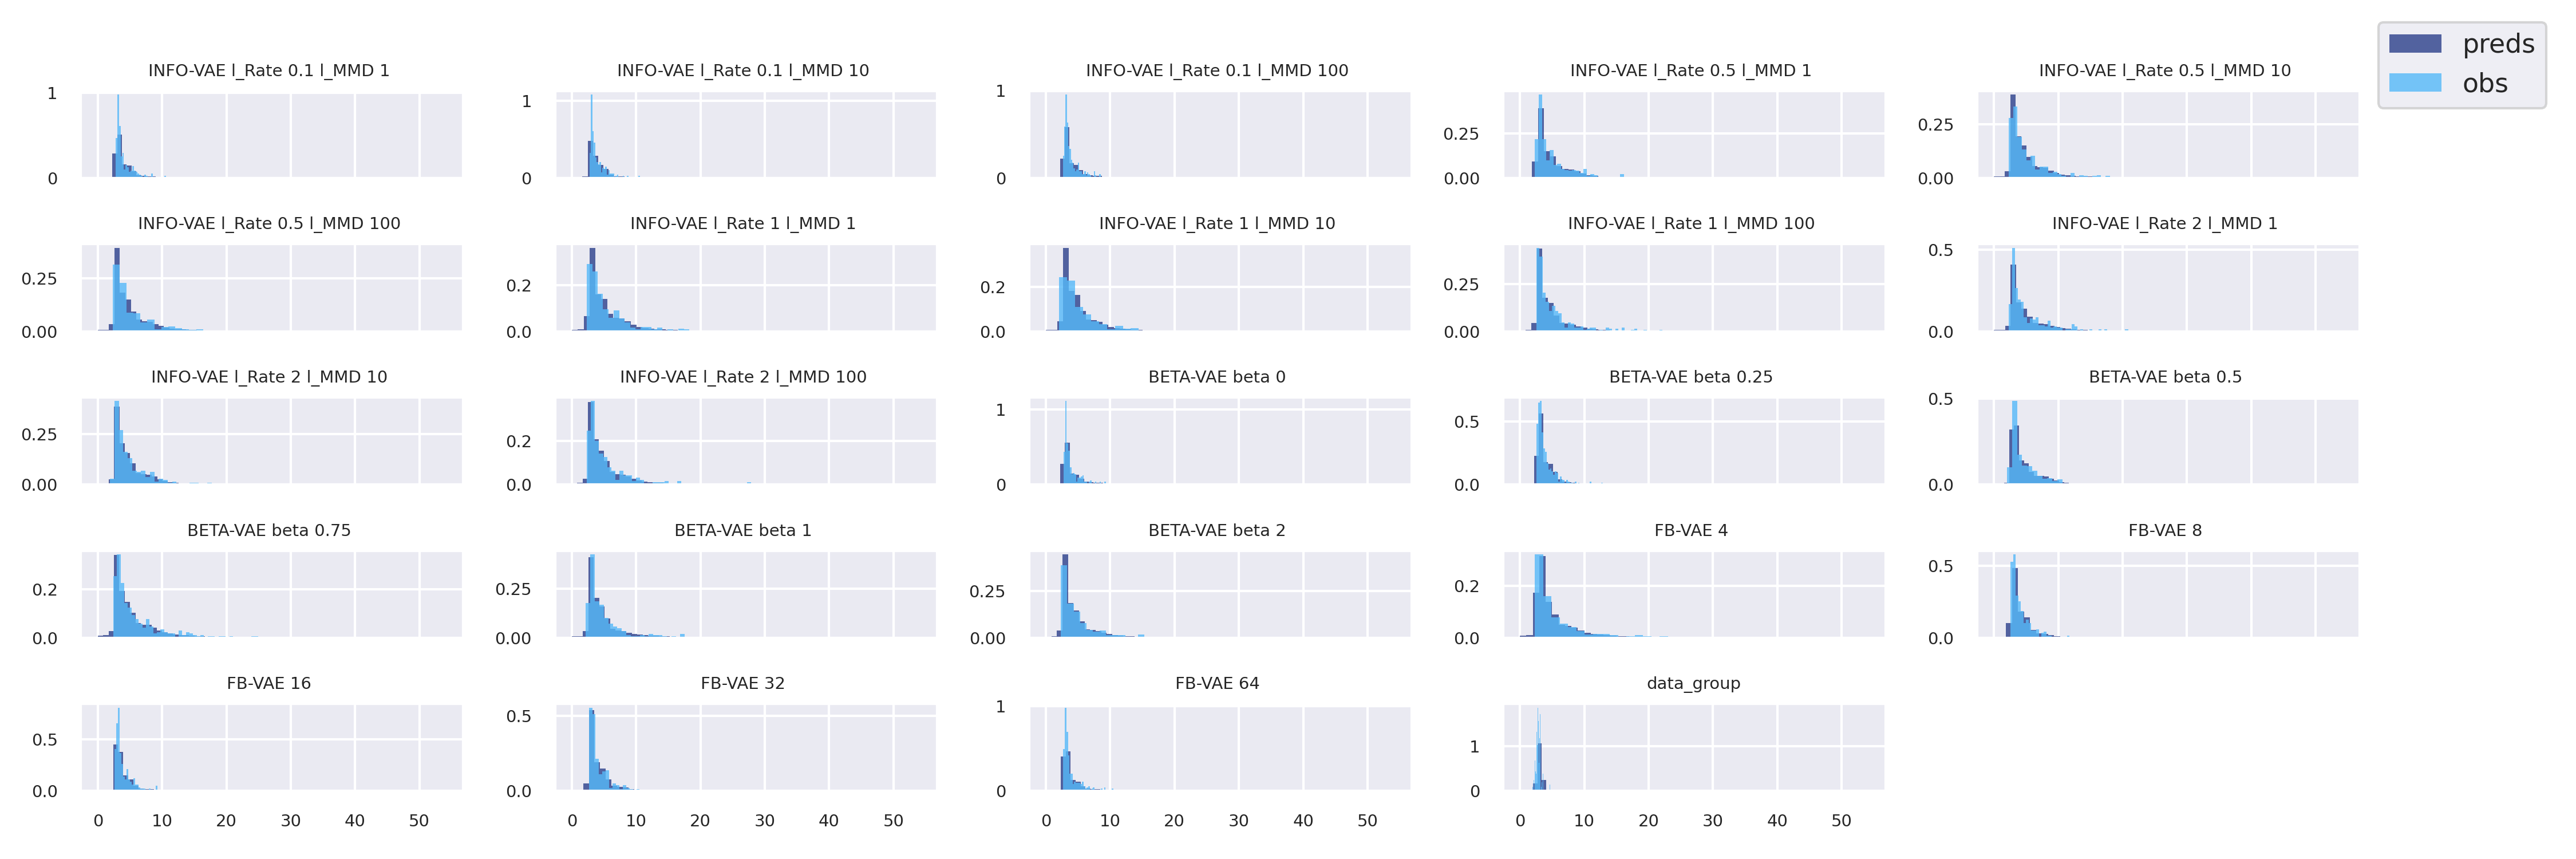
\includegraphics[width=\textwidth]{images/bda_checks/surprisal_dps/ptb_seq_len_prediction_checks__conditional_conditional.png}
    \caption{Posterior predictive samples (preds) versus observations (obs) of the $T(\tilde x^*|x^*)$ statistic assessed under the Penn Treebank sequence length latent structure model as modelled by the DP mixture model.}
    \label{fig:surprisal_check_ptb_seq_len_con_con}
\end{figure*}

% SURPRISAL DP CHECKS PTB TOPICS 1
\begin{figure*}[!htb]
    \centering
    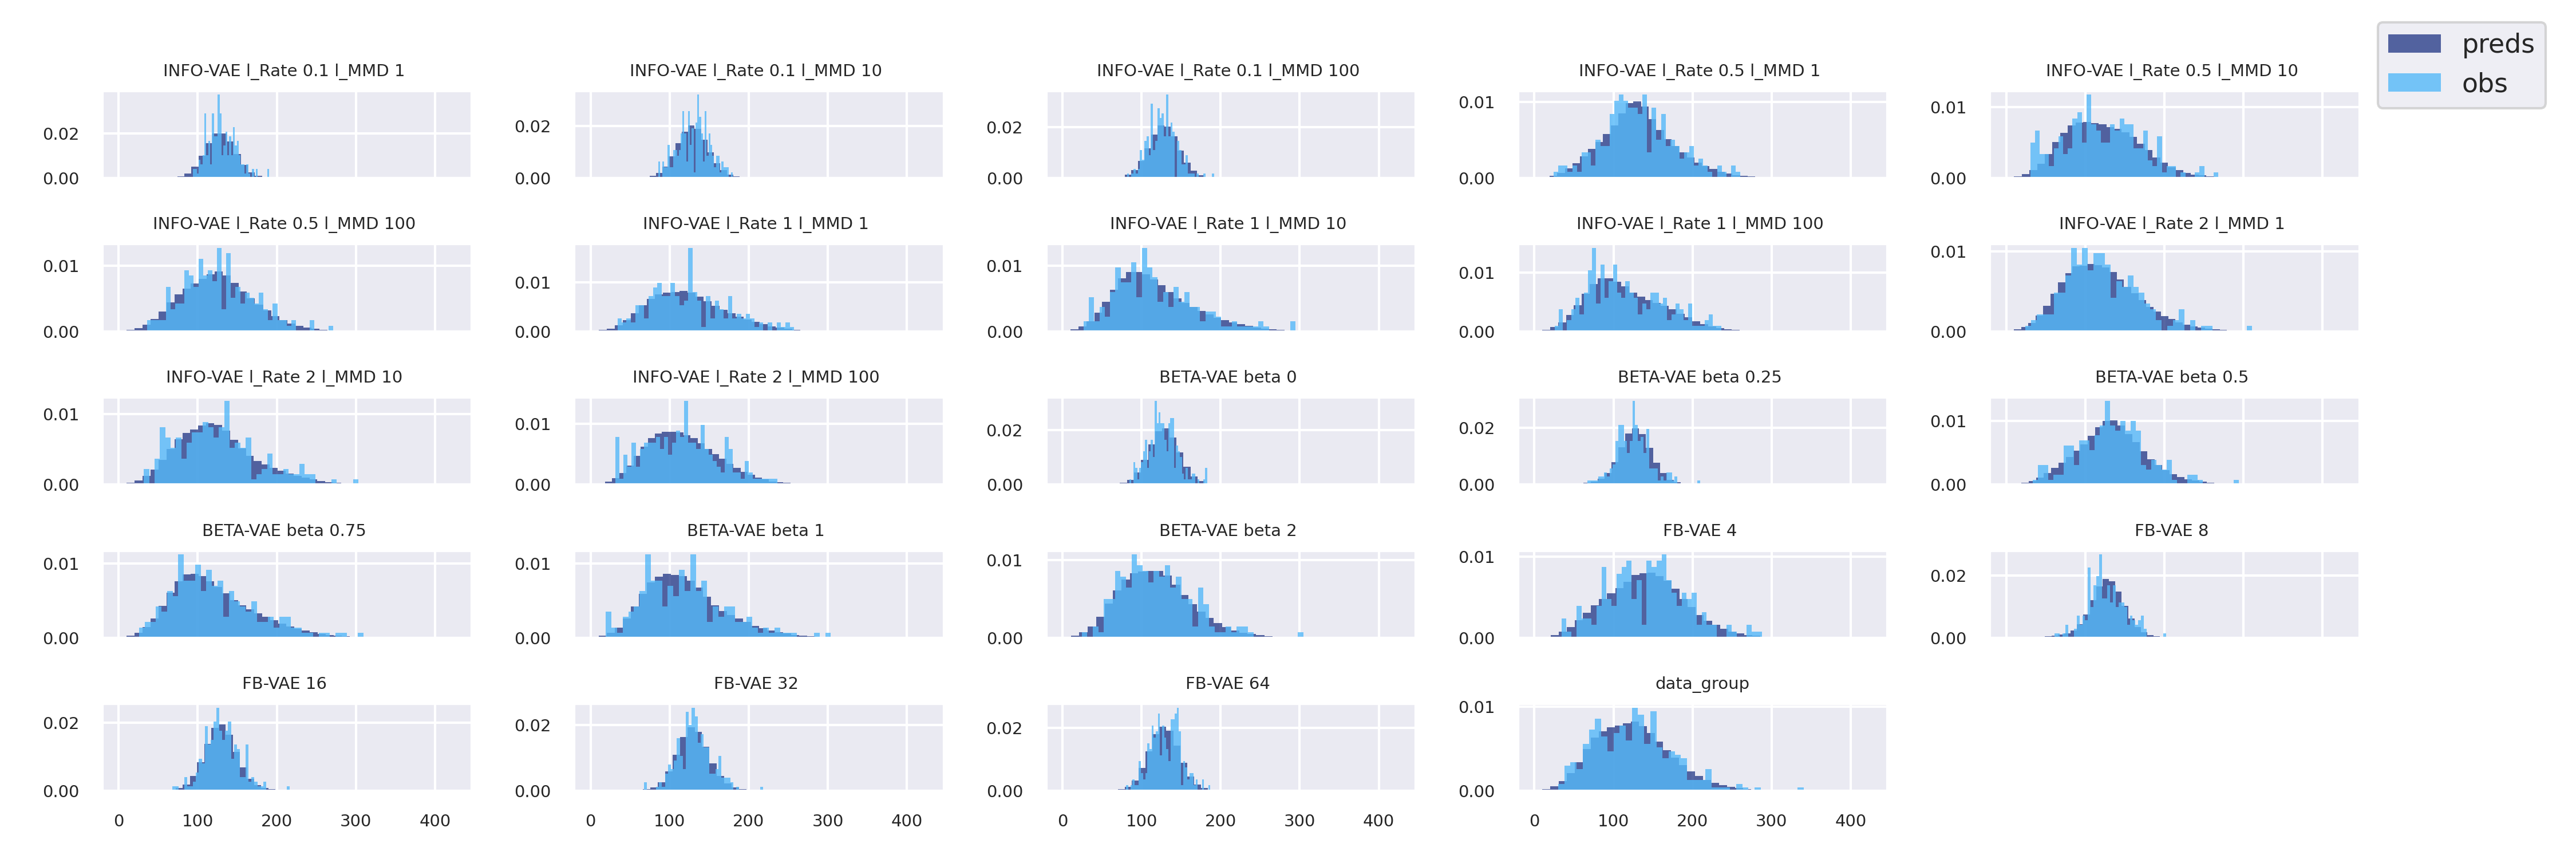
\includegraphics[width=\textwidth]{images/bda_checks/surprisal_dps/ptb_topics_prediction_checks__unconditional_unconditional.png}
    \caption{Posterior predictive samples (preds) versus observations (obs) of the $T(x^*)$ statistic assessed under the Penn Treebank topic latent structure model as modelled by the DP mixture model.}
    \label{fig:surprisal_check_ptb_topics_uncon_uncon}
\end{figure*}

% SURPRISAL DP CHECKS PTB TOPICS 2
\begin{figure*}[!htb]
    \centering
    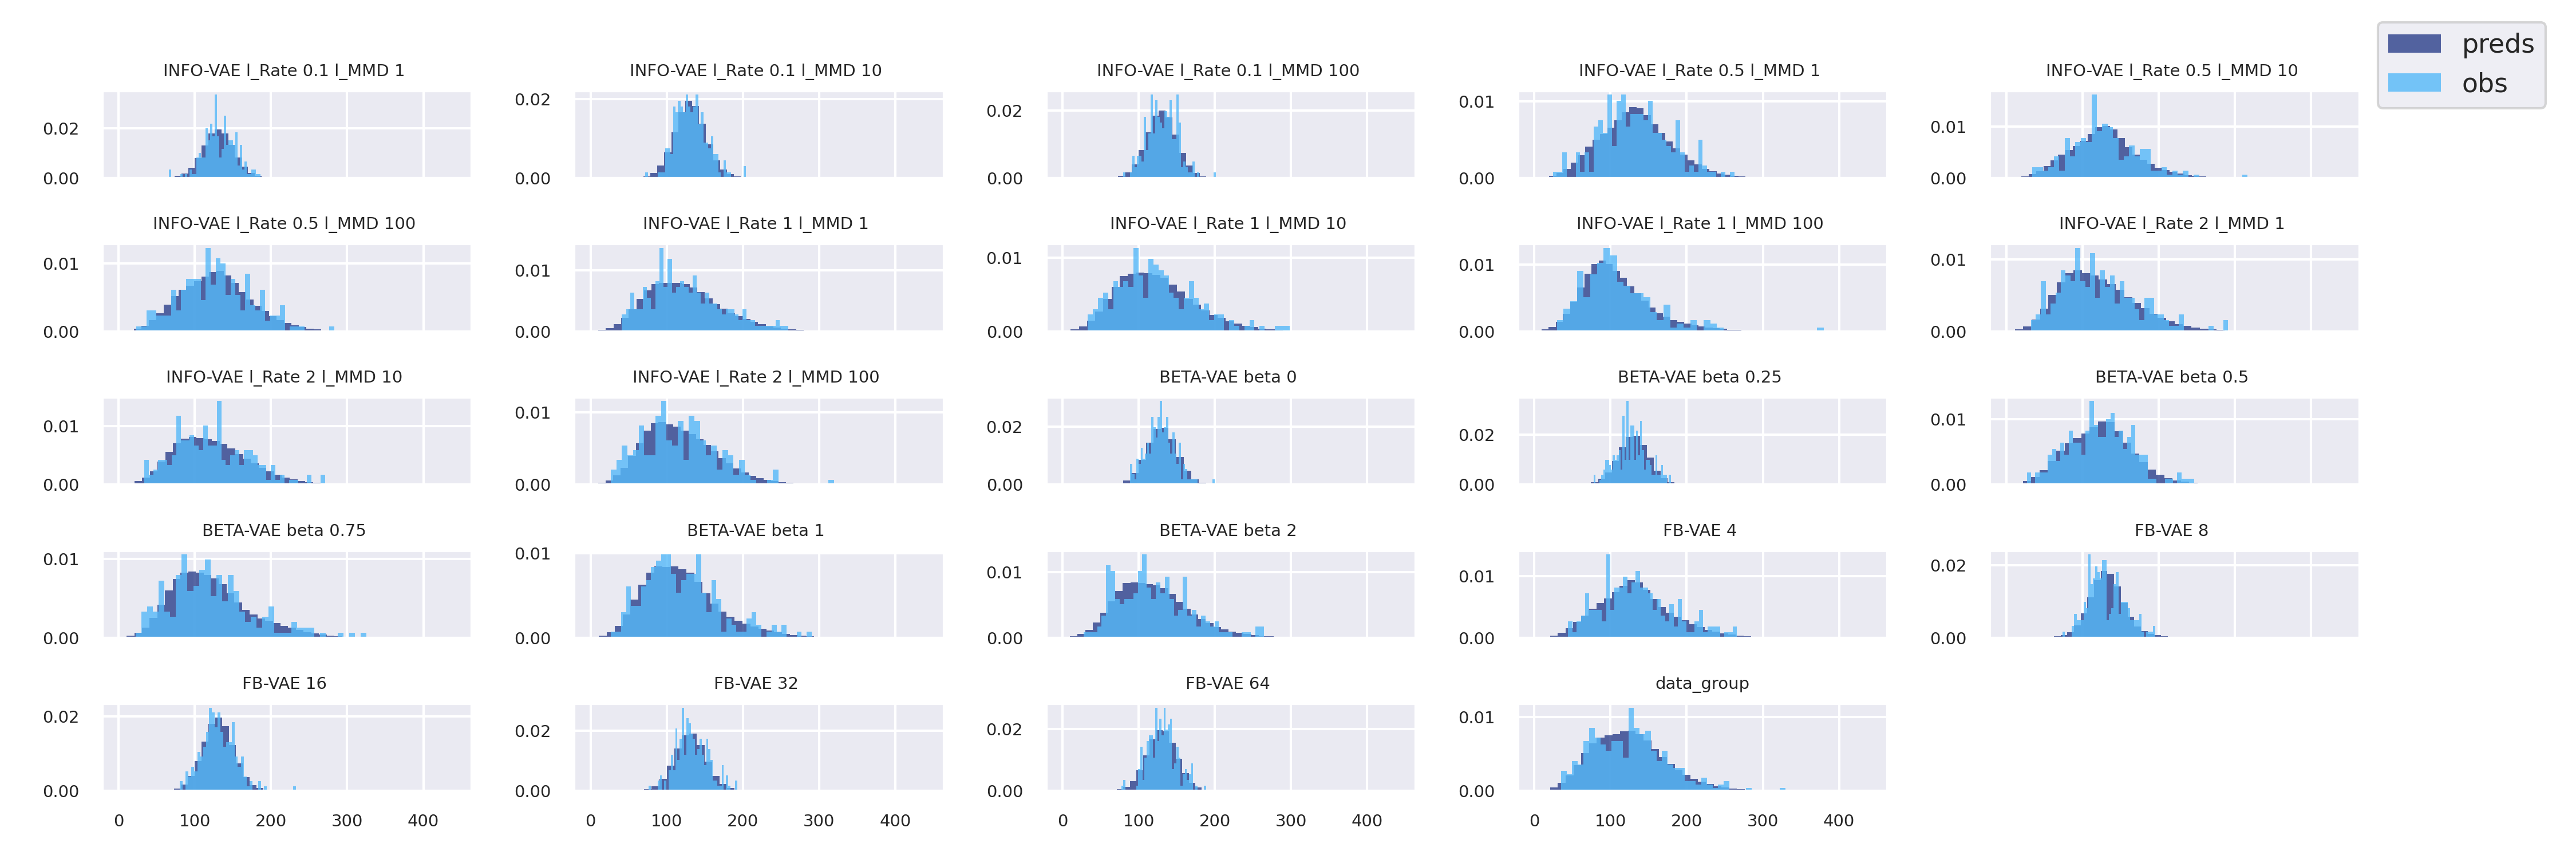
\includegraphics[width=\textwidth]{images/bda_checks/surprisal_dps/ptb_topics_prediction_checks__unconditional_conditional.png}
    \caption{Posterior predictive samples (preds) versus observations (obs) of the $T(\tilde x^*)$ statistic assessed under the Penn Treebank topic latent structure model as modelled by the DP mixture model.}
    \label{fig:surprisal_check_ptb_topics_uncon_con}
\end{figure*}

% SURPRISAL DP CHECKS PTB TOPICS 3
\begin{figure*}[!htb]
    \centering
    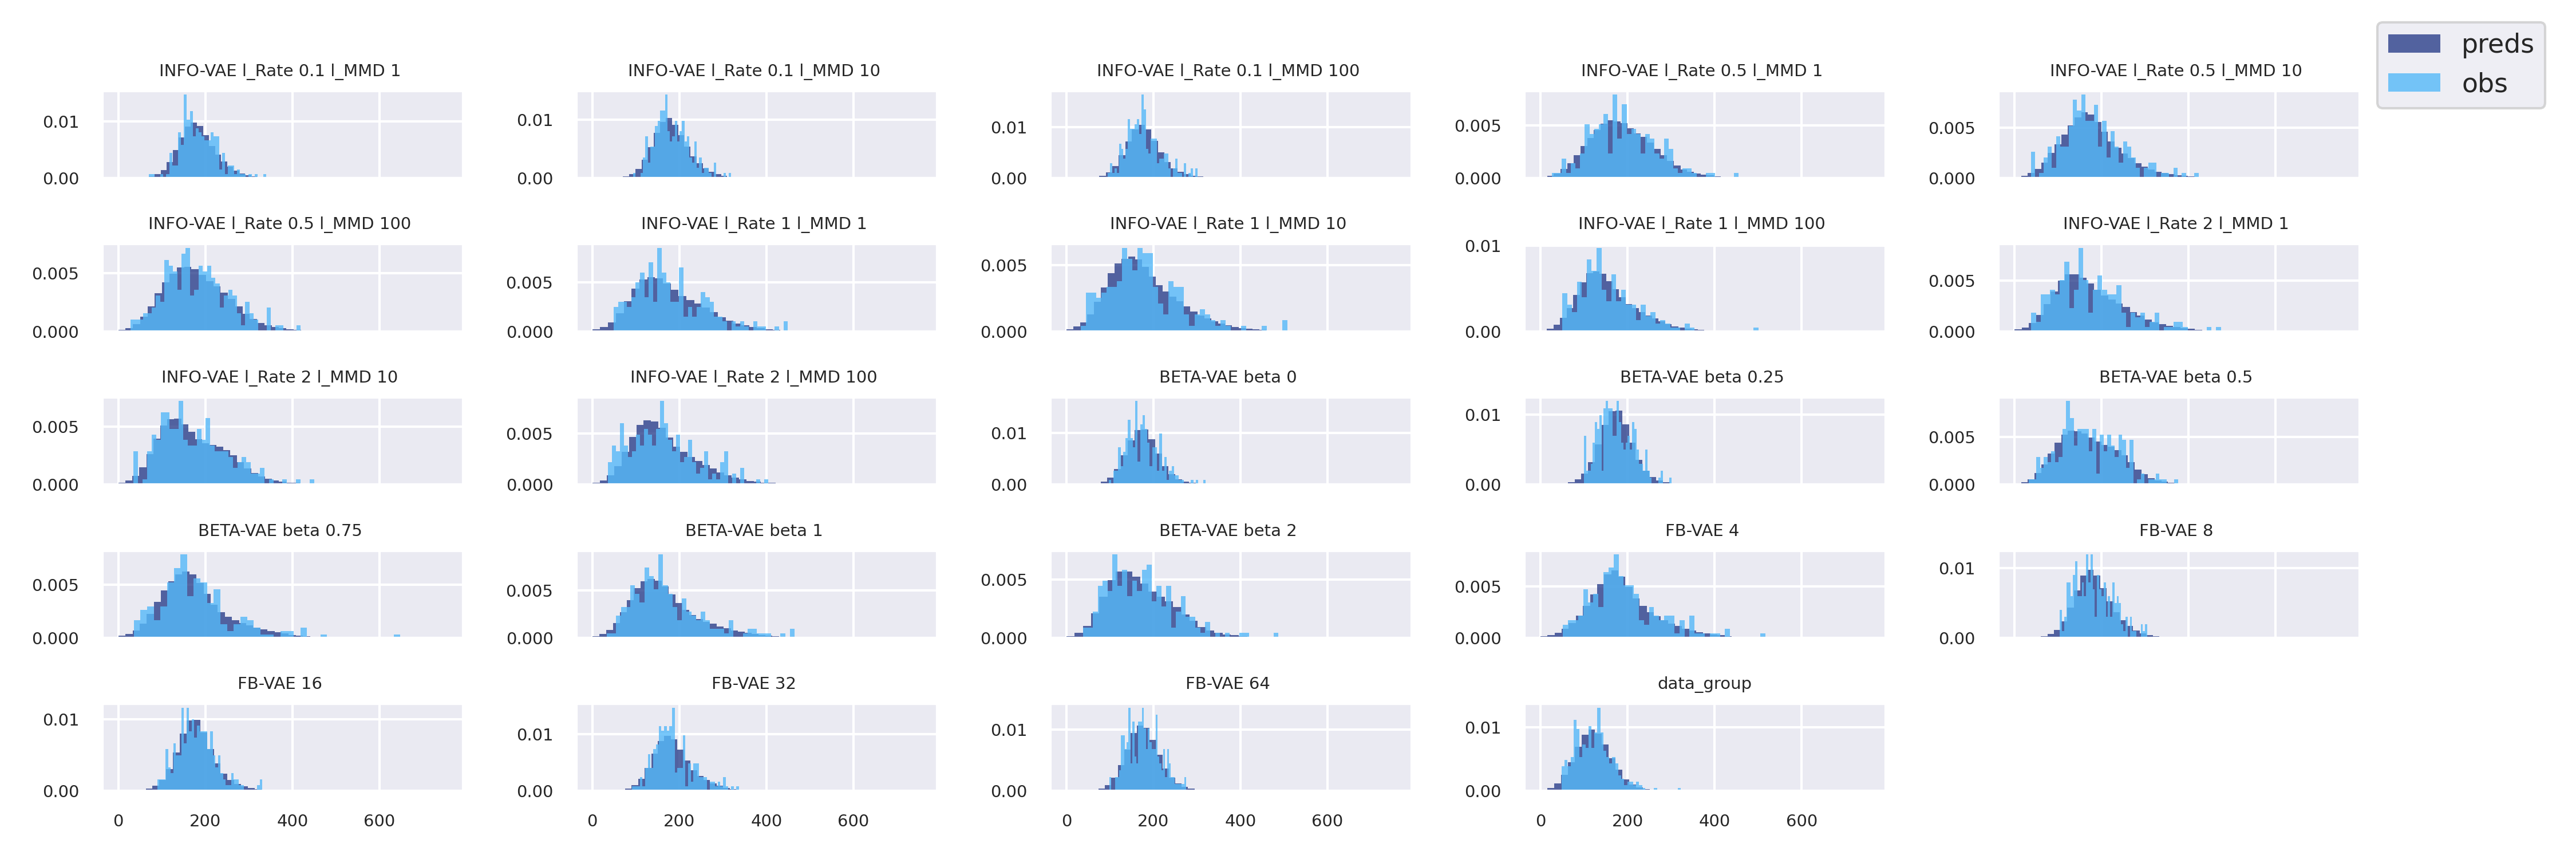
\includegraphics[width=\textwidth]{images/bda_checks/surprisal_dps/ptb_topics_prediction_checks__conditional_conditional.png}
    \caption{Posterior predictive samples (preds) versus observations (obs) of the $T(\tilde x^*|x^*)$ statistic assessed under the Penn Treebank topic latent structure model as modelled by the DP mixture model.}
    \label{fig:surprisal_check_ptb_topics_con_con}
\end{figure*}

\section{Estimated divergence to control group}\label{app:kl-plots}

In Figures \ref{fig:kl-plot-mnist} -- \ref{fig:kl-plot-ptb-topics} we plot full experimental results of the plots equivalent to those presented in Figure \ref{fig:all-kl-plots} in Section \ref{sec:experiments}.

% MNIST KL plots
\begin{figure*}[!htb]
    \centering
    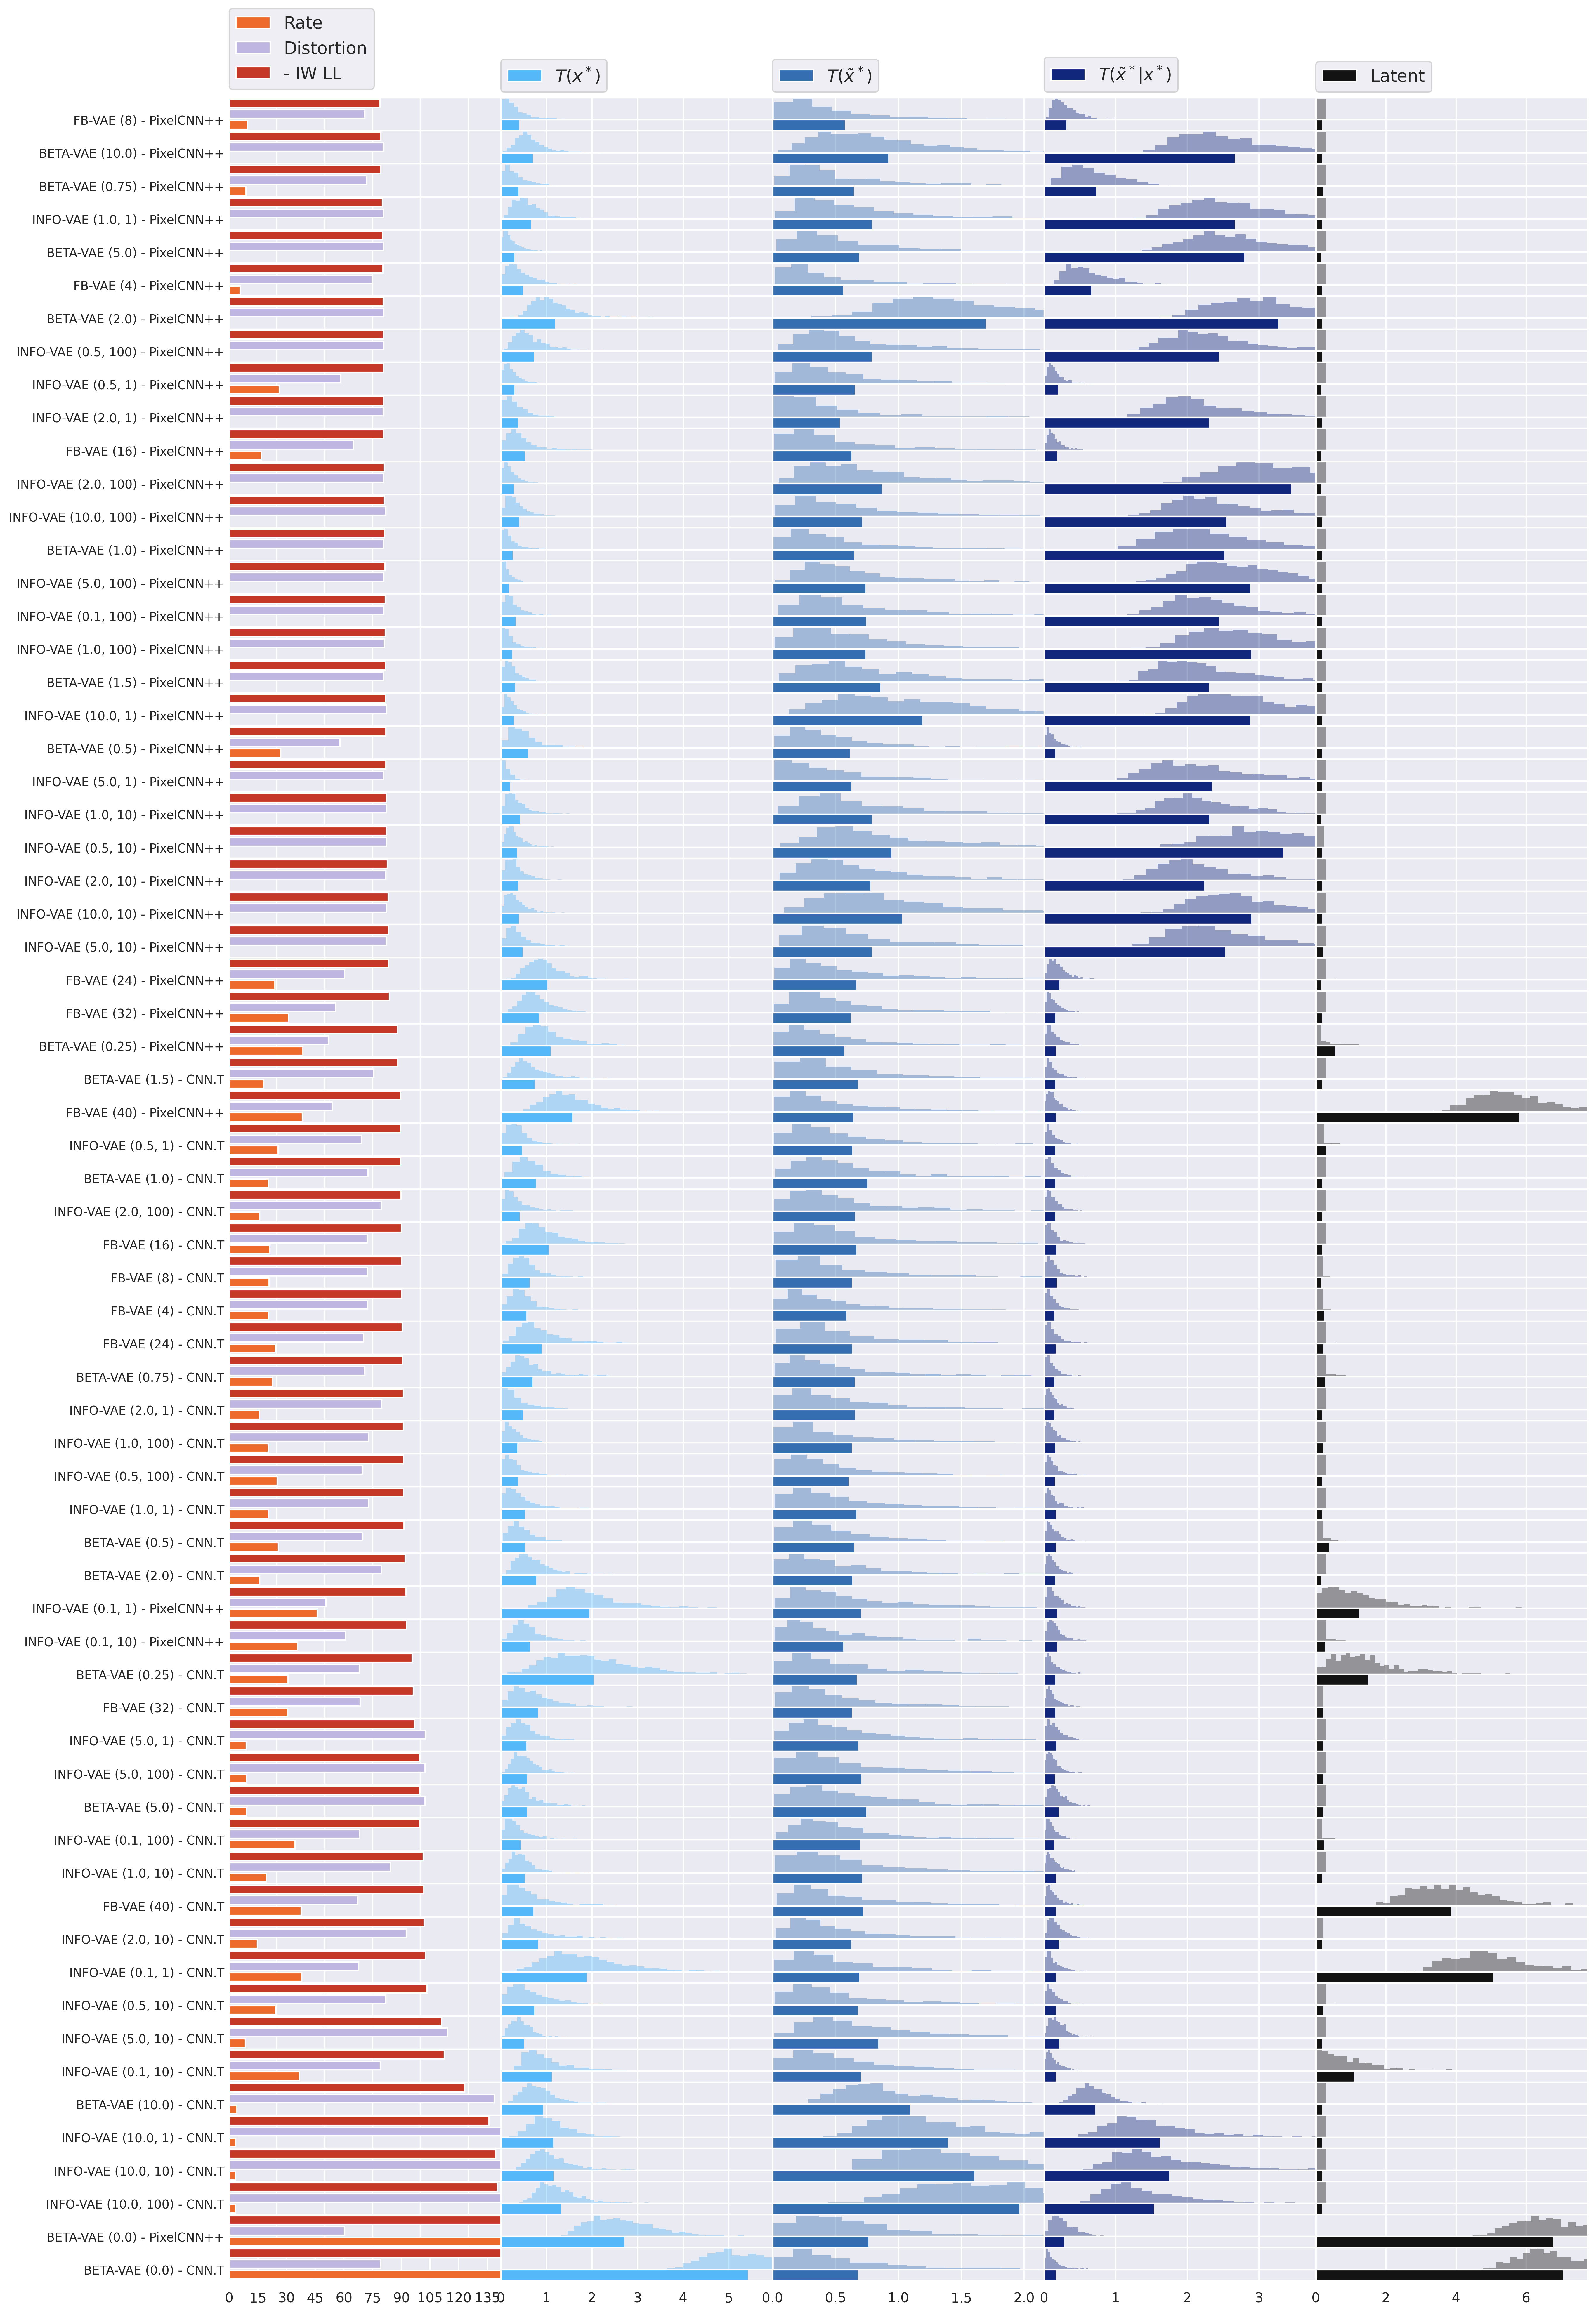
\includegraphics[width=0.8\textwidth]{images/kl_plots/mnist_selection_False.png}
    \caption{Full experimental results for the control group divergence analysis for the MNIST digit identity structure model. The left most column shows the intrinsic evaluation metrics for reference. The middle three columns show estimated divergences from the control group under our analysis model. The right most column shows the control group divergence under the latent analysis model. The horizontal bars denote the average value of the sampled divergences plotted as histograms. The experiments are labelled with the objectives according to the following format: \infovae ($\lambda_{\text{rate}}$, $\lambda_{\text{MMD}}$), \betavae ($\beta$) and \fbvae ($\lambda_{\text{FB}}$). We additionally distinguish between decoder types used: CNN.T or PixelCNN++.}
    \label{fig:kl-plot-mnist}
\end{figure*}

% PTB sequence length KL plots
\begin{figure*}[!htb]
    \centering
    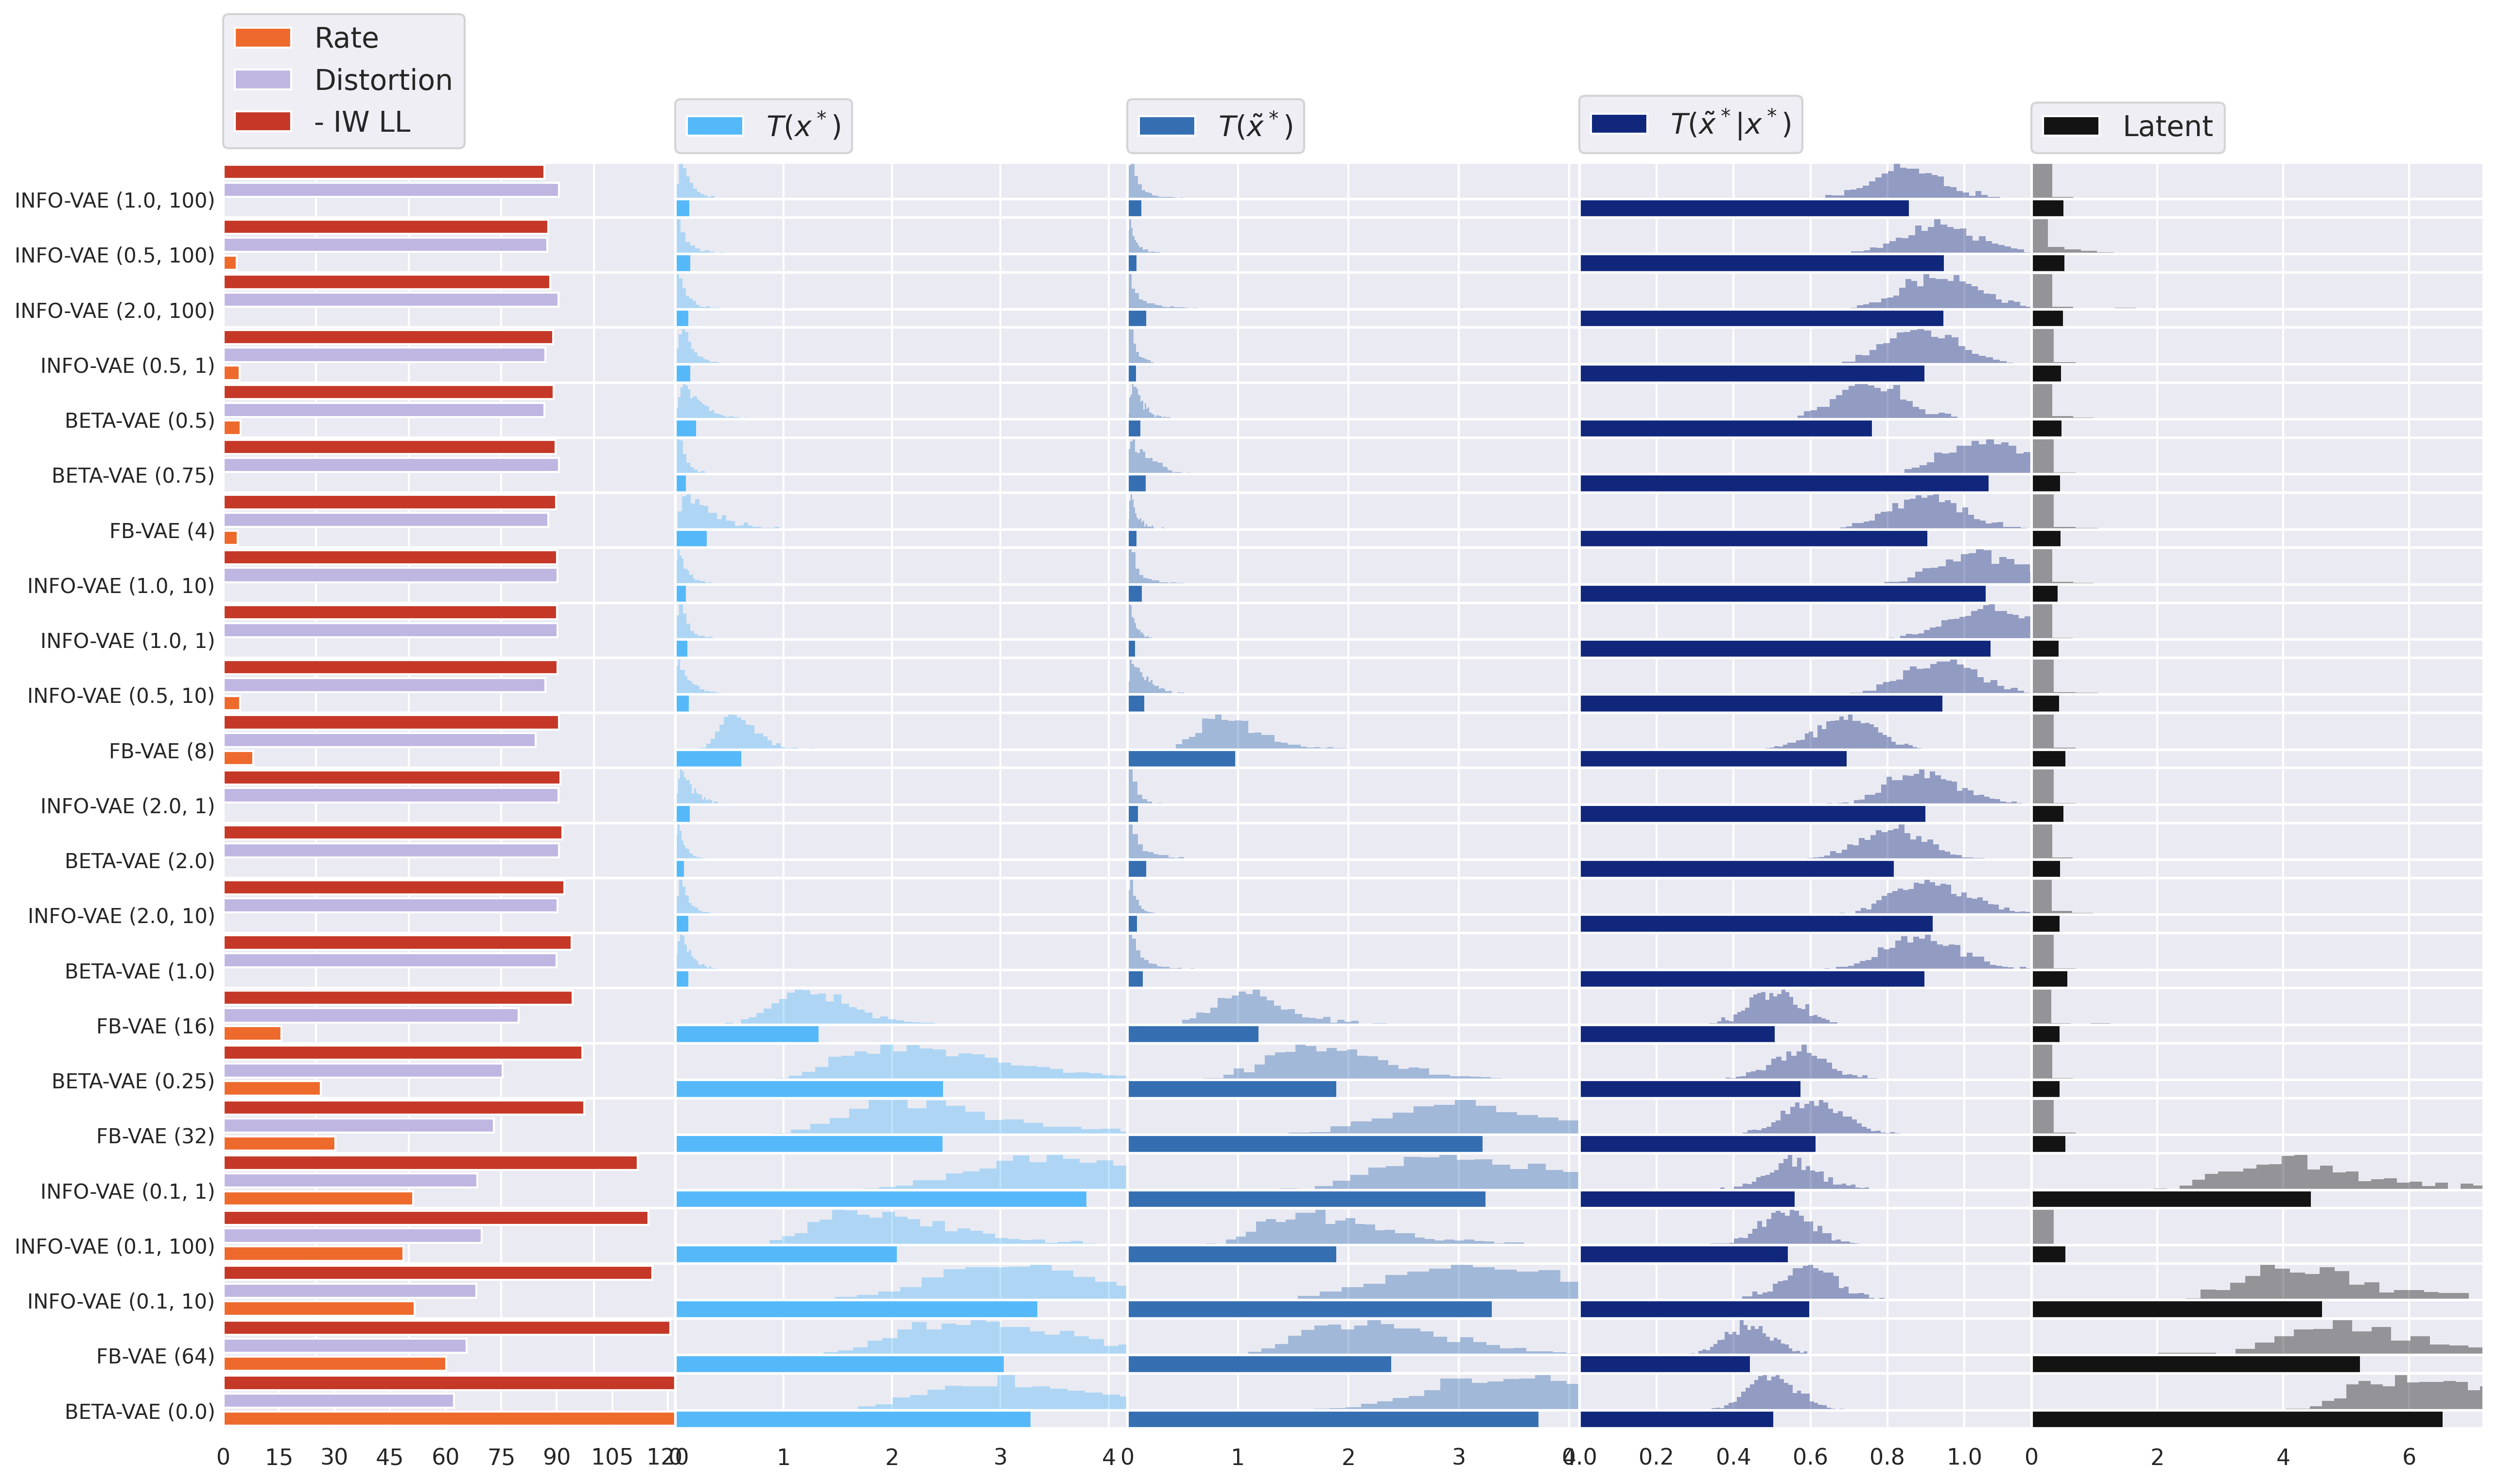
\includegraphics[width=\textwidth]{images/kl_plots/ptb_sequence_len_selection_False.png}
    \caption{Full experimental results for the control group divergence analysis for the PTB sequence length latent structure model. The left most column shows the intrinsic evaluation metrics for reference. The middle three columns show estimated divergences from the control group under our analysis model. The right most column shows the control group divergence under the latent analysis model. The horizontal bars denote the average value of the sampled divergences plotted as histograms. The experiments are labelled with the objectives according to the following format: \infovae ($\lambda_{\text{rate}}$, $\lambda_{\text{MMD}}$), \betavae ($\beta$) and \fbvae ($\lambda_{\text{FB}}$). }
    \label{fig:kl-plot-ptb-seq-len}
\end{figure*}

% PTB LDA KL plots
\begin{figure*}[!htb]
    \centering
    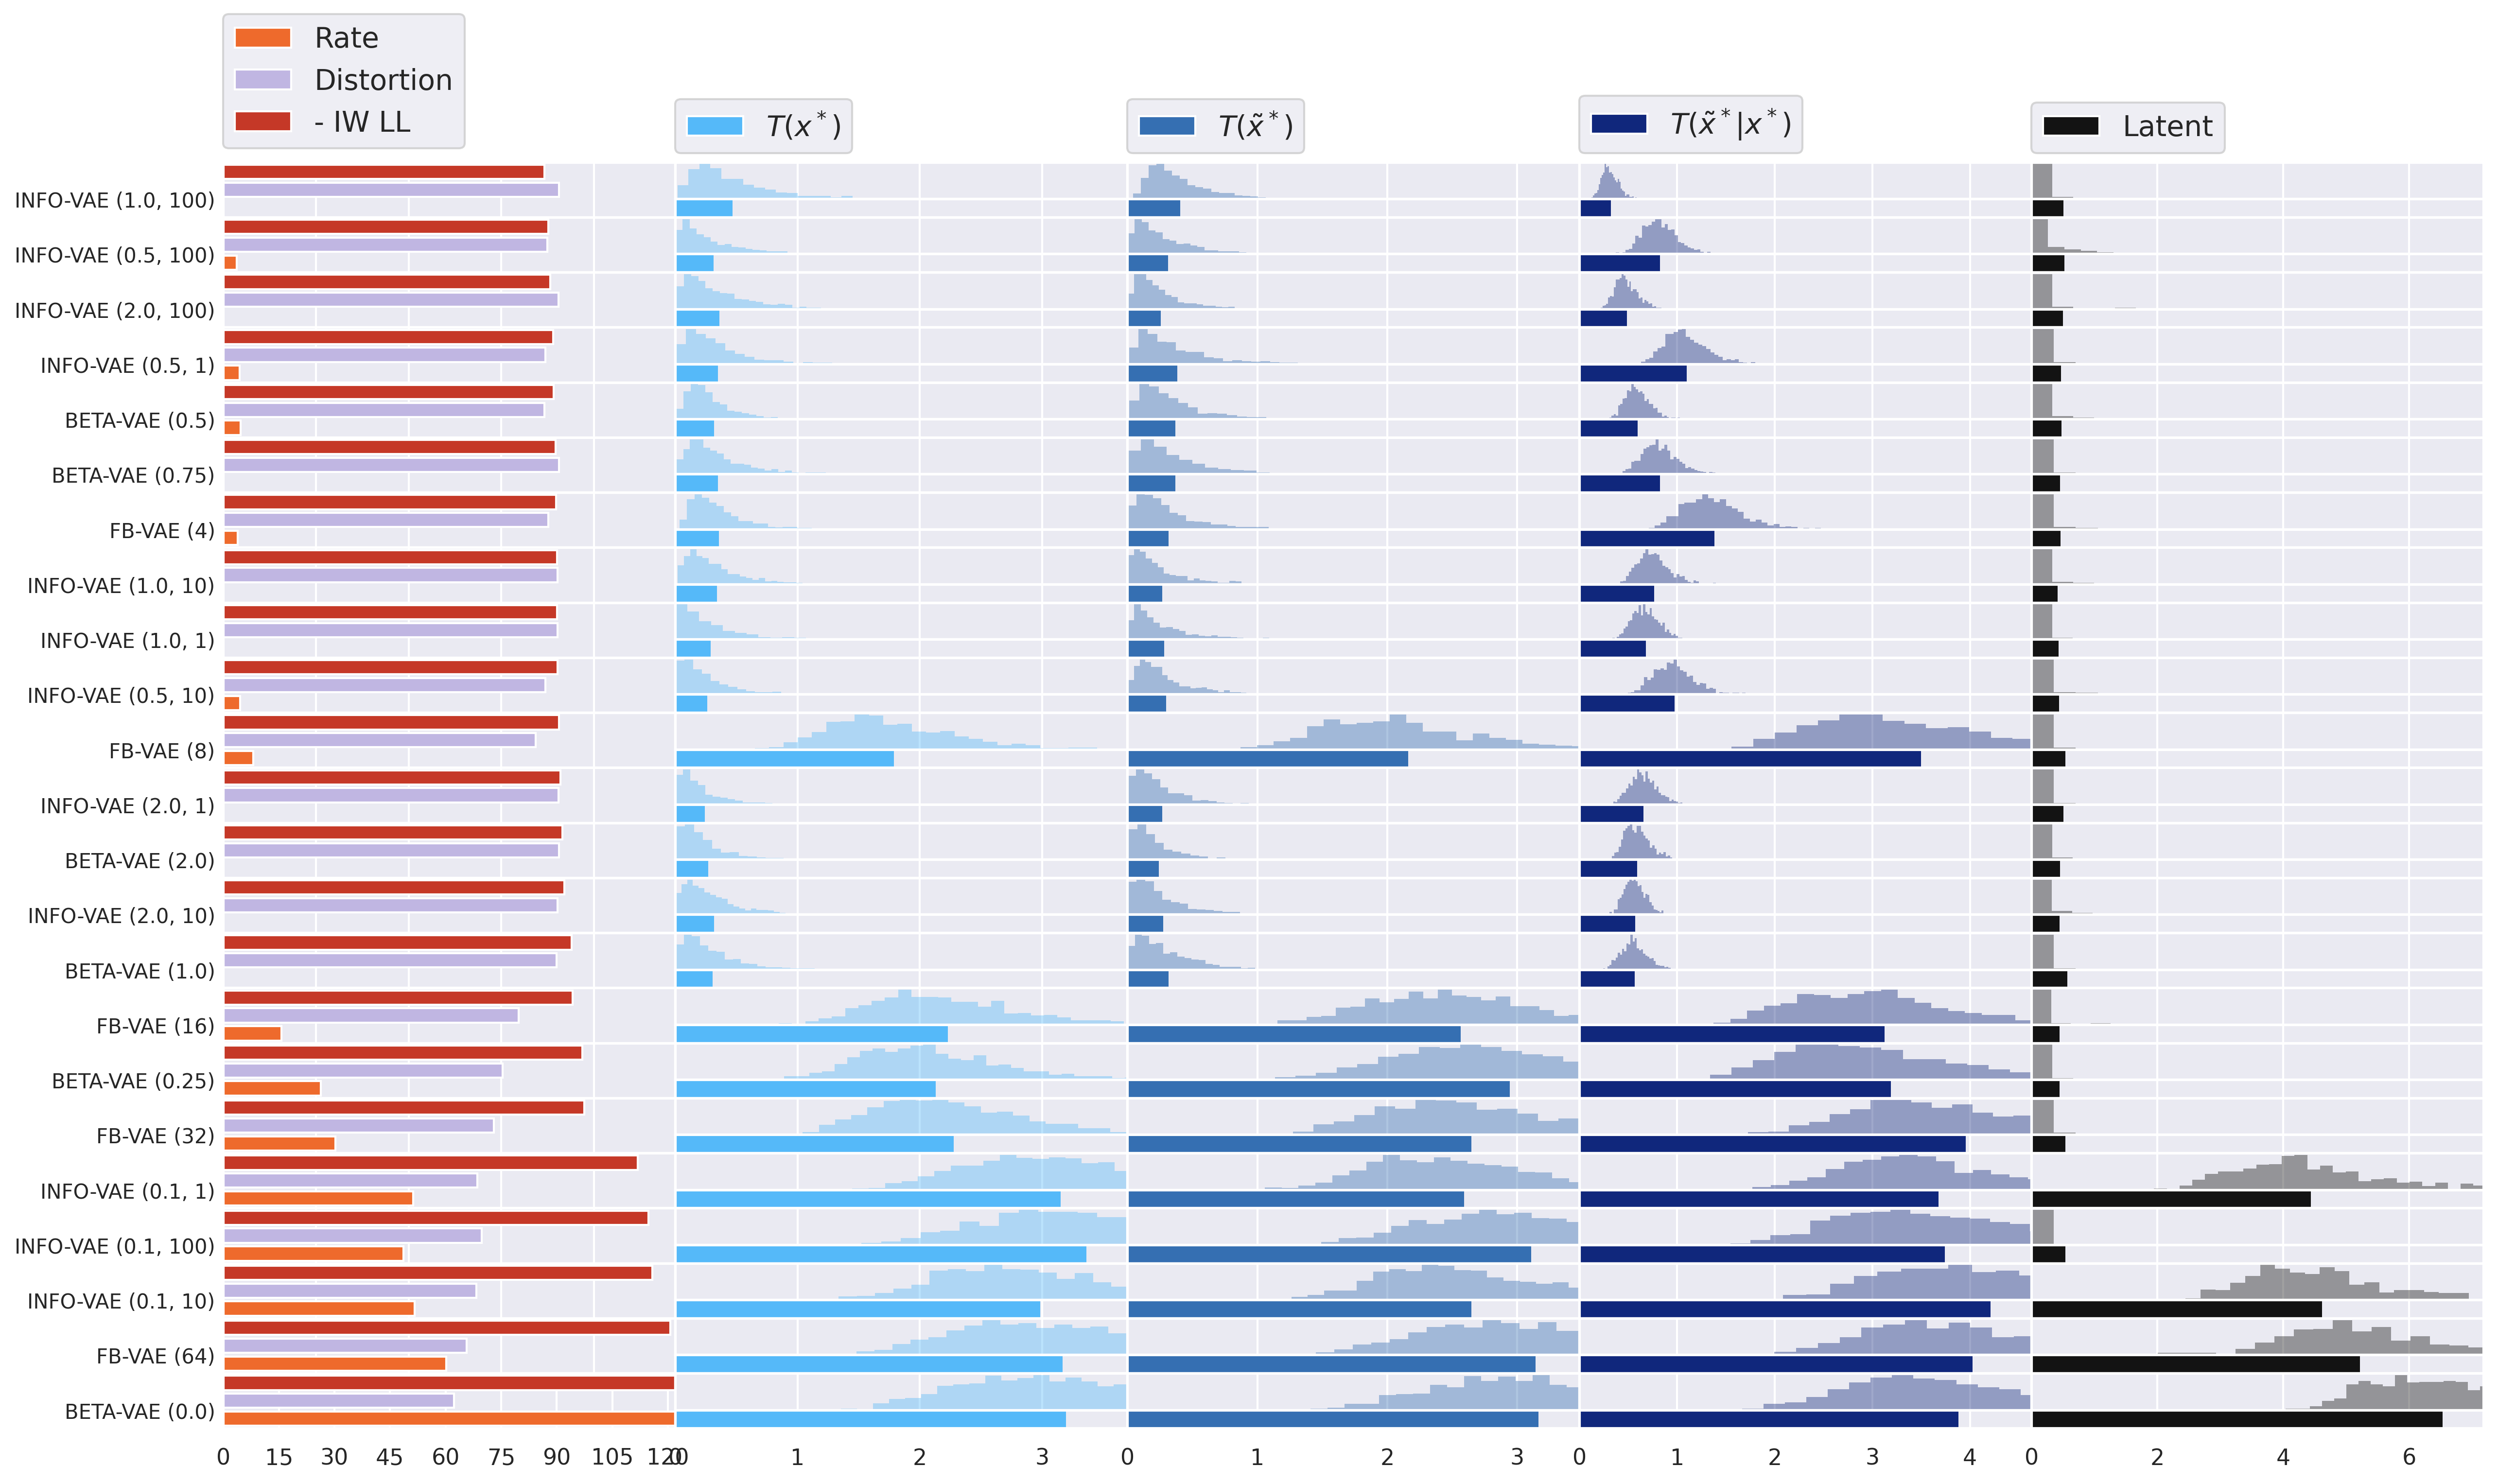
\includegraphics[width=\textwidth]{images/kl_plots/ptb_topics_selection_False.png}
    \caption{Full experimental results for the control group divergence analysis for the PTB topic structure model. The left most column shows the intrinsic evaluation metrics for reference. The middle three columns show estimated divergences from the control group under our analysis model. The right most column shows the control group divergence under the latent analysis model. The horizontal bars denote the average value of the sampled divergences plotted as histograms. The experiments are labelled with the objectives according to the following format: \infovae ($\lambda_{\text{rate}}$, $\lambda_{\text{MMD}}$), \betavae ($\beta$) and \fbvae ($\lambda_{\text{FB}}$). }
    \label{fig:kl-plot-ptb-topics}
\end{figure*}
